
\documentclass[11pt,a4paper]{amsart}

\usepackage[margin=1in]{geometry}
\usepackage{amsmath,amssymb,amsthm,mathtools}
\usepackage{graphicx,mathrsfs}
\usepackage[expansion=false]{microtype}
\usepackage{booktabs,longtable,array}
\usepackage{tikz}
\usetikzlibrary{arrows.meta,calc,positioning,patterns,decorations.pathreplacing}
\usepackage[colorlinks=true,linkcolor=black,citecolor=black,urlcolor=black]{hyperref}
\usepackage[nameinlink,capitalize]{cleveref}

\hypersetup{
  pdftitle={Minimal-period rigidity for ribbon-outer skew Schur compositions},
  pdfauthor={John Shields},
  pdfkeywords={skew Schur function, marked composition, source-minimal period, boundary synchronization, Jacobi--Trudi determinant, ribbon outer, composition necessity}
}
\pdfinfo{/ORCID (https://orcid.org/0009-0004-3882-4571)}
\numberwithin{equation}{section}
\theoremstyle{plain}
\newtheorem{theorem}{Theorem}[section]
\newtheorem{proposition}[theorem]{Proposition}
\newtheorem{lemma}[theorem]{Lemma}
\newtheorem{corollary}[theorem]{Corollary}
\theoremstyle{definition}
\newtheorem{definition}[theorem]{Definition}
\newtheorem{remark}[theorem]{Remark}
\newtheorem{example}[theorem]{Example}
\newtheorem{question}[theorem]{Question}
\newcommand{\Lam}{\Lambda}
\newcommand{\Z}{\mathbb Z}
\newcommand{\Q}{\mathbb Q}
\newcommand{\one}{\mathbf1}
\newcommand{\AT}{\operatorname{AT}}
\newcommand{\Row}{\operatorname{Row}}
\newcommand{\Col}{\operatorname{Col}}
\newcommand{\spn}{\operatorname{sp}}
\newcommand{\ord}{\operatorname{ord}}
\newcommand{\Core}{\operatorname{Core}}
\newcommand{\Cl}{\operatorname{Cl}}
\newcommand{\JT}{\operatorname{JT}}
\newcommand{\Splice}{\operatorname{Splice}}
\newcommand{\score}{\operatorname{score}}
\newcommand{\wt}{\operatorname{wt}}
\newcommand{\Jlower}{\mathsf J_{<n}}
\newcommand{\DD}{\mathscr D}
\newcommand{\eps}{\varepsilon}
\newcommand{\floor}[1]{\left\lfloor#1\right\rfloor}
\newcommand{\sminus}{S^{-}_{\mathrm{cap}}}
\newcommand{\splus}{S^{+}_{\mathrm{cap}}}
\DeclareMathOperator{\adj}{adj}
\DeclareMathOperator{\diag}{diag}
\DeclareMathOperator{\sgn}{sgn}
\setlength{\emergencystretch}{1.5em}
\allowdisplaybreaks[2]

\title[Minimal-period rigidity for ribbon-outer skew Schur compositions]{Minimal-period rigidity for ribbon-outer\\skew Schur compositions}
\author{John Shields}
\date{October 19, 2026}
\thanks{Independent researcher, Ginza 2-15-2, KR Ginza II 5F, Chuo-ku, Tokyo, Japan 104-0061.\\
\hspace*{\parindent}Corresponding author: \href{mailto:math@johnnyshields.com}{math@johnnyshields.com}.  ORCID: \href{https://orcid.org/0009-0004-3882-4571}{0009-0004-3882-4571}.\\
\hspace*{\parindent}This work is archived at \href{https://doi.org/10.5281/zenodo.23482349}{doi:10.5281/zenodo.23482349}.}
\subjclass[2020]{Primary 05E05; Secondary 05A17, 15A15}
\keywords{skew Schur function, marked composition, source-minimal period,
boundary synchronization, Jacobi--Trudi determinant, ribbon outer,
composition necessity}

\begin{document}
\begin{abstract}
We prove that minimal factorizations of Schur-equal connected skew diagrams
have the same period (the content shift in the defining translation between
inner copies) when the larger-period outer is a ribbon.  At each diagram,
the overlap's diagonal span is minimized first, then the inner diagram's.
At every strictly smaller area, we assume that every connected Schur class
containing diagrams unrelated by rotation admits a nontrivial composition,
and that Schur equality preserves the existence of nontrivial compositions
and, for minimal factorizations, the marked inner together with the outer
Schur function, modulo the permitted identifications.  The compositions
satisfy Hypotheses I--IV of McNamara and van Willigenburg, with an arbitrary
competing outer; we exclude classes containing a nontrivial composition
whose inner is a row or column.  Jacobi--Trudi determinant identities
synchronize both diagram boundaries and yield a legal composition on the
original diagram contradicting minimality; equal-period factor
identification remains separate.
\end{abstract}
\maketitle


\section{Introduction}\label{sec:introduction}

Distinct connected skew diagrams, not related by rotation, can have
the same skew Schur function \cite[Ex.~7.8]{Reiner2007Coincidences}.
Marked composition explains many such equalities by assembling copies of an
inner diagram according to an outer diagram and allowing suitable factor
reversals.  A natural inverse question is whether equality of the resulting
functions determines the scale at which a source-minimal composition is
assembled.  We prove a period-selection theorem when the larger-period
chart~\cite{Shields2026Gluing} has a ribbon outer, under a classification
hypothesis at strictly smaller areas.

The composition of McNamara and van Willigenburg
\cite{McNamara2009Classification} records an inner diagram, two marked end
copies, their displacement, and their attachment type.  A proper chart
\(F=D\circ_\omega E\) has connected factors of at least two cells.  If its period
is \(p\) and the marked overlap has span \(w\), then
\begin{equation}\label{eq:intro-span}
 N_F=pN_D+w,\qquad N_E=p+w.
\end{equation}
The period is the content of the displacement between copies, not the full
span of the inner.  The chart is \emph{source-minimal} when
\begin{equation}\label{eq:intro-score}
 \score(D,E,\omega)=(w,N_E)=(w,p+w)
\end{equation}
is lexicographically least among the proper charts of the same source \(F\).
On the line-inner-free domain, these are exactly the least-period charts,
by the least-root-period corollary of \cite{Shields2026Gluing}.
The forward composition and reversal identities under Hypotheses I--IV are
available from Olson-Harris \cite{OlsonHarris2024HopfApplications}.  Our problem
is to recover geometric information from an equality of their outputs.

Local common-factor gluing compares two charts already carried by the same
diagram \cite{Shields2026Gluing}.  It gives equal fibers at equal periods,
reassociation at divisible periods, and a legal common-divisor chart in the
remaining compatible cases.  These conclusions do not directly compare
prescribed charts on different Schur-equal parents: the second chart has not
yet been realized on the first diagram.

Corner transport gives a further reduction
\cite{Shields2026CornerDescent}.  If \(D_1,\ldots,D_t\) are the connected components
of the outer interior \(D^-\), the extreme Jacobi--Trudi cofactor of
\(D\circ_\omega E\) contains the transported child factors
\(s_{D_i\circ_\omega E}\), with exact multiplicities.  A ribbon has empty interior.
In the ribbon-outer case this particular descent has no outer-interior child
to follow, although local cap and normalization factors remain.  The present
argument replaces that child-factor step by boundary reconstruction.

\subsection{Main theorem}

For a connected Schur class, \emph{rootedness transfer} means that the existence
of one proper chart implies that every class member has a proper chart.
\emph{Root existence} means that a class that is not a single rotation orbit
has a rooted member.  \emph{Rooted-key invariance} means that rooted members
have the same marked source-minimal key, with the ordinary gauge acting on
both the marked inner and outer function.  Let \(\Jlower\) denote these three
assertions for every connected Schur class of area strictly below \(n\).
Their full-fiber and factor-reversal consequences are recalled in
\Cref{sec:descent}.  No current-area instance is included in \(\Jlower\).

\begin{theorem}[Ribbon-outer period rigidity]\label{thm:main}
Assume \(\Jlower\).  Suppose a connected Schur class contains no member with a
proper line-inner chart.  Let
\begin{equation}\label{eq:original-comparison}
 F=D\circ_\omega E,\qquad H=C\circ_\eta U,\qquad
 s_F=s_H,\qquad |F|=n,
\end{equation}
be proper source-minimal charts satisfying Hypotheses I--IV.  If their periods
satisfy \(p\ge q\) and \(D^-=\varnothing\), then \(p=q\).
\end{theorem}

The competing outer \(C\) is arbitrary.  Only the hypothesis on \(D\) initially
allows \(N_D=|D|\) in \eqref{eq:intro-span}; \(N_C\) is not replaced by \(|C|\)
before ribbon inheritance is proved.  Neither \(F\) nor \(H\) is assumed to be a
ribbon.  The conclusion compares the two prescribed source-minimal periods,
not all periods of arbitrary proper presentations.

The hypothesis \(\Jlower\) is the joint induction hypothesis, not a shorthand
for period rigidity alone.  In particular, root existence at smaller areas is
needed when a smaller inner might be chartless.  This induction step does not by
itself establish the joint package at all areas.

\subsection{What diagonal heights forget}

Let \([\ell_k,h_k]\) be the rows of a diagram on content \(k\), and put
\begin{equation}\label{eq:intro-bits}
 \begin{gathered}
 A_k=\ell_{k-1}-\ell_k,\qquad B_k=h_{k-1}-h_k,
 \qquad H_k=h_k-\ell_k+1,\\
 H_k-H_{k-1}=A_k-B_k.
 \end{gathered}
\end{equation}
Here \(A_k,B_k\in\{0,1\}\).  The two choices \((0,0)\) and \((1,1)\) have the same
difference.  Thus a periodic height word need not have periodic boundary words.
In beta coordinates, the forgotten choices are precisely the common entries
of the row and column lists.  Removing such an entry preserves every diagonal
height, area and span, but changes both membership words.

The proof first reduces \eqref{eq:original-comparison} to a positive
nondividing comparison with distinct attachment phases and two original line
outers (\Cref{thm:reduction}).  Writing \(g=\gcd(p,q)\) and
\(N=Lg+c\), \(0<c<g\), it obtains periodic
structure for the \emph{whole} cores and heights.  The remaining task is to
synchronize the paired records of the restored parents.  This is stronger than
identifying a core class or the determinant of a return block.

\subsection{The synchronization mechanism}

The two original composition annihilators act
on the same normalized whole function.  Their commutator, compared at the
\(q\) and \(p+q\) horizons, aligns the ordinary clocks and supplies a complementary
cap response.  Original \(p\)-periodicity identifies the two finite low-index
decks; it does not identify their different high-index alphabets.

The constant coefficient in \(z\) of the cap response detects
offending records at the extreme
connected components of the weak return core.  Its first coherent-unit
coefficient has a pole with a residue that is a sum of particular weak-minor
products.  A simultaneous separated specialization gives these products one
positive sign.  Coincident end factors therefore add their contributions,
rather than cancel them.  Only the outward cap discrepancies that could defeat
the next sign argument are removed.

In the original determinant, the same whole differential
identity is a sum of full row and column replacements.  Each surviving
replacement is a feasible weak Jacobi--Trudi determinant.  After the cap
exclusions all nonzero weighted terms have one sign.  Ordinary comparisons give
boundary equality; mixed comparisons give a directed inclusion
(\Cref{thm:scalar-synchronization}).  A one-way
inequality cannot stay strict around a finite period cycle, so both conclusions
yield gcd synchronization.

The synchronized words and the actual singleton diagonals then construct a
legal period-\(g\) chart on the same source (\Cref{thm:fold}).
Only after that construction is
its score compared with \eqref{eq:intro-score}.  This bypasses an exhaustive
classification of the intermediate rational return responses.

\subsection{Organization and relation to companion preprints}

\Cref{sec:charts} fixes the common geometric and determinant conventions.
\Cref{sec:descent} separates strict descent and actual reconstruction from
minimality.  \Cref{sec:reduction} reduces the original arbitrary-\(C\)
comparison to the line-outer branch.
The aligned construction in \Cref{app:aligned} uses the cell-only cut
theorem of \Cref{app:cell-cut} and applies weak-cap reconstruction
\cite{Shields2026Coframes} to the actual end windows; the exceptional constructions in
\Cref{app:empty,app:coincident} use the contact rigidity of
\Cref{app:contacts}.
\Cref{sec:geometry,sec:response} derive periodic structure, actual cap systems
and the two-horizon response.  \Cref{sec:poles,sec:whole-sign} prove the pole
filter and complete shifted-determinant noncancellation.
\Cref{sec:fold} constructs the finer chart and completes \Cref{thm:main}.
\Cref{app:alternative} gives an optional alternative geometric
realization of the same scalar obstruction, using the shared
structural, operator, end-pole and contact inputs.

Companion preprint \cite{Shields2026Gluing} supplies same-parent geometry and
source-minimal fiber domination.  Preprint \cite{Shields2026CornerDescent} supplies
the cofactor transport and exact normalization.  The erosion, zero-free
class transport and inflation-of-legal-charts lemmas of
\cite{Shields2026Inflation} supply the actual zero-free class reduction;
their exact transport domain does not assert that arbitrary inflation
preserves Schur equality.  The weak-cap and absolute-flag theorem of
\cite{Shields2026Coframes} supplies reconstruction from complete rational
coframes, including units and disconnected proper blocks.
The supplied-period covariance and terminal readout of
\cite{Shields2026Readout} are used in the whole-source extraction below.
After the periods agree, marked-factor and prescribed-fiber
identification remain separate questions.


\section{Marked charts, boundary words, and Jacobi--Trudi data}\label{sec:charts}

\subsection{Diagrams and full beta lists}

Diagrams are finite skew Young diagrams in English notation, identified up to
translation.  Connected means nonempty and edge-connected.  We write \(|S|\),
\(r(S)\), \(c(S)\) and \(N_S\) for area, number of rows, number of columns and number
of occupied diagonals.  The content of \((i,j)\) is \(j-i\).  For connected \(S\),
\(N_S=r(S)+c(S)-1\).  Rotation through \(180\) degrees is denoted by \(S^*\);
antitransposition is \(\AT(i,j)=(-j,-i)\).  The symbols \(\Row_j\) and \(\Col_j\) denote the \(j\)-cell row and column.  The symmetric-function involution \(\iota\) satisfies \(\iota(h_j)=e_j\) and \(\iota(s_S)=s_{\AT(S)}\), where \(e_j\) is the elementary symmetric function.  Write \(\iota_\gamma\) for the identity or \(\iota\) according as \(\gamma=\mathrm{id}\) or \(\AT\).

A row profile lists the row lengths, followed after a semicolon by the
adjacent overlap lengths minus one; these latter quantities are called gaps.

Normalize the southwest content to zero.  The full beta lists are strictly
decreasing integer lists
\[
 X=(N,x_1,\ldots,x_{r-1}),\qquad
 Y=(y_0,\ldots,y_{r-2},0),\qquad
 s_S=\det(h_{x-y})_{x\in X,\,y\in Y}.
\]
We always retain \(h_0=1\) and \(h_j=0\) for \(j<0\).
A row with endpoints \((x,y)\) occupies contents \(y,\ldots,x-1\).
Consequently
\begin{equation}\label{eq:height-beta}
 H_S(k)=\#\{y\in Y:y\le k\}-\#\{x\in X:x\le k\},
 \qquad 0\le k<N.
\end{equation}
The two internal boundary words are \(A_k=\one_{k\in Y}\) and
\(B_k=\one_{k\in X}\), with the diagonal-interval convention of
\eqref{eq:intro-bits}.  They are defined at \(1\le k<N\); there are no artificial
boundary steps at \(0\) or \(N\).

A pair of binary boundary words and positive heights beginning and ending at
one reconstruct a connected skew diagram.  Indeed, starting from the southwest
singleton, the diagonal interval endpoints change by zero or minus one at each
step.  Their intervals then form the two skew boundaries; every cell off the
last diagonal has an eastern or northern neighbor on the next diagonal.  We
will use this criterion for unions and shortening splices as well as for
original diagrams.

A \emph{common beta} is an element of \(X\cap Y\).  Deleting it from both lists
preserves \eqref{eq:height-beta}, hence the entire height word, area, span and
connectedness.  Repeating the deletion gives the \emph{zero-free core}
\(\Core(S)\).  Zero-free means absence of common betas; negative-index zero
entries are not removed.  Restoring a common beta changes the two membership
words by \(00\leftrightarrow11\).

\begin{lemma}\label{lem:core-class}
If connected diagrams \(S,T\) have equal Schur functions, their zero-free cores
have equal Schur functions.  Their original row counts and numbers of common
betas also agree.
\end{lemma}
\begin{proof}
The original row count is the maximum ordinary degree, where \(\deg h_j=1\)
for \(j>0\).  If \(u=|X\cap Y|\), selecting all \(u\) nonattacking unit entries in the
determinant leaves, up to its actual Laplace sign, the homogeneous nonzero
determinant of the zero-free core, of degree \(r-u\).  Every other selection has
larger ordinary degree.  Thus the least ordinary degree and its entire
homogeneous part determine \(u\) and the core Schur polynomial up to sign.
Actual skew Schur functions are positive at a sufficiently large positive
alphabet, so two such associates have sign \(+1\).
\end{proof}

\subsection{Legal marks and composition}

We use the conventions of \cite{Shields2026Gluing}, following
\cite{McNamara2009Classification}.  A marked inner \(\omega\) consists of a
connected diagram \(E\), connected end copies \(W_-\) and \(W_+=W_-+v\), and their
attachment data.  The lower copy contains the southwest cell and the upper
copy the northeast cell.  Put
\[
 O=E\setminus(W_-\cup W_+),\qquad w=N_W,\qquad p=N_E-w=c(v).
\]
The cases \((a),(b),(c),(d)\) have lower/upper attachment types
\((H,H),(V,V),(H,V),(V,H)\), respectively.  Cases \((a),(b)\) are ordinary and
\((c),(d)\) are mixed.  Horizontal attachment uses the western or eastern neighbor
of the relevant extreme middle cell; vertical attachment uses its southern or
northern neighbor.

The mark is legal under the following conditions.
\begin{enumerate}
\item[(I)] No strictly larger skew diagram containing \(W_-\) on the same content
 diagonals has translated copies at both ends of \(E\).
\item[(II)] There is an occupied diagonal between the two copies meeting neither:
 \(0\le w<p\).
\item[(III)] Removing either marked copy leaves a connected skew diagram.
\item[(IV)] In \(\boldsymbol E=\bigcup_{k\in\Z}(E+kv)\) no hatted-middle copy
 is adjacent to a hatted-mark copy, where, for \(e=(1,1)\),
 \[
 \widehat O_1=\{x\in O_1:x+e\in O_1\},\qquad
 \widehat W_1=\{x\in\boldsymbol E:x+e\in W_1\}
       \cup\{x\in W_1:x+e\in\boldsymbol E\}.
 \]
\end{enumerate}
Adjacency means sharing an edge.  No Hypothesis V is imposed.
At \(w=0\) the mark is the horizontal edge reading, of displacement
\(v_H=\operatorname{ne}(E)-\operatorname{sw}(E)+(0,1)\).
A vertical edge reading has displacement \(v_H-e\) and is converted by the
ordinary gauge, which antitransposes the outer.
\Cref{fig:chart} gives a row-inner example.
\begin{figure}[!b]
\centering
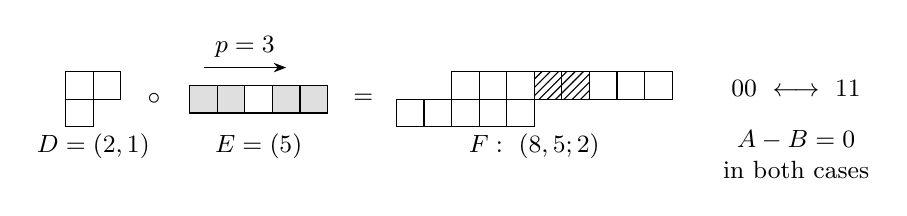
\begin{tikzpicture}[x=.35cm,y=.35cm,font=\small]
 \begin{scope}[shift={(0,0)}]
  \foreach \x/\y in {0/0,0/1,1/1}{\draw (\x,\y) rectangle ++(1,1);}
  \node at (1,-.7) {\(D=(2,1)\)};
 \end{scope}
 \node at (3.2,1) {\(\circ\)};
 \begin{scope}[shift={(4.5,.5)}]
  \foreach \x in {0,1,3,4}{\fill[gray!25] (\x,0) rectangle ++(1,1);}
  \foreach \x in {0,...,4}{\draw (\x,0) rectangle ++(1,1);}
  \draw[-{Stealth[length=1.6mm]}] (.5,1.65)--(3.5,1.65)
    node[midway,above] {\(p=3\)};
  \node at (2.5,-1.2) {\(E=(5)\)};
 \end{scope}
 \node at (10.8,1) {\(=\)};
 \begin{scope}[shift={(12,0)}]
  \foreach \x in {0,...,4}{\draw (\x,0) rectangle ++(1,1);}
  \foreach \x in {2,...,9}{\draw (\x,1) rectangle ++(1,1);}
  \fill[pattern=north east lines] (5,1) rectangle (7,2);
  \node at (5,-.7) {\(F:\ (8,5;2)\)};
 \end{scope}
 \begin{scope}[shift={(25,0)}]
  \node[align=center] at (1.5,1.4) {\(00\ \longleftrightarrow\ 11\)};
  \node[align=center] at (1.5,-1.0) {\(A-B=0\)\\in both cases};
 \end{scope}
\end{tikzpicture}
\caption{A legal row-inner chart, illustrating period and overlap rather than
 the hypotheses of the hard comparison.  The marked inner has \(p=3\) and \(w=2\).  The ribbon outer has three cells;
 its row action gives profile \((8,5;2)\) and span \(3\cdot3+2=11\).
 The hatched cells are the overlap of the two copies in the upper row.  The inset records the elementary
 ambiguity left by diagonal heights.  No equality between two different
 source-minimal charts is asserted by this illustration.}\label{fig:chart}
\end{figure}

For a cell \(d=(i,i+j)\) of the outer \(D\), let \([\ell_j^D,h_j^D]\) be its
content-\(j\) diagonal interval.  The copy origin is
\[
 L_\omega(d)=
 \begin{cases}
 jv+ie,&(a),\\
 jv-ie,&(b),\\
 jv+(i-\ell_j^D)e,&(c),\\
 jv-(h_j^D-i)e,&(d).
 \end{cases}
\]
In cases \((c),(d)\) the vertical boundary-ribbon pairs contribute the supplemental
copies \(W_++L_\omega(d)+e\) and \(W_++L_\omega(d)-e\), respectively, with \(d\) the
lower cell.  These copies are part of the composition.  A proper chart
\(D\circ_\omega E\) has \(|D|,|E|\ge2\).


\subsection{Local geometry and the coding table}

We record the precise parts of local gluing used below.  Their proofs are the
local geometry, coding and mark-window arguments of
\cite{Shields2026Gluing}.

\begin{proposition}\label{prop:local-data}
For a legal positive mark of period \(p\) and width \(w\), the following hold.
\begin{enumerate}
\item \(W_-=E\cap(E-v)\).  The middle has at most one cell on each marked
 diagonal.  The private diagonals \(w\) and \(p-1\) are singletons.
\item The middle occupies \([s,p+t-1]\), where \(1\le s\le w\), \(0\le t<w\);
 for mixed marks \(t<s\).
\item If \(N_D=M\), then \(N_{D\circ_\omega E}=Mp+w\).  Its first \(p\) diagonals
 and its last \(p\) diagonals are the corresponding two translated windows of
 \(E\), and their nonempty private overlap reconstructs \(E\).
\item The full boundary words are \(p\)-periodic away from the exceptional
 residues in \eqref{eq:coding}.  The initial and terminal values are those
 in \eqref{eq:caps}.
\end{enumerate}
\end{proposition}
\begin{equation}\label{eq:coding}
\begin{array}{c|cc}
 & A & B\\\hline
(a)&t&s\\
(b)&s&t\\
(c)&\varnothing&t,s\\
(d)&t,s&\varnothing
\end{array}
\qquad
\begin{array}{c|cc}
 &\text{interior first slot}&\text{interior second slot}\\\hline
(a)&A_{jp+t}=A_j^D&B_{jp+s}=B_j^D\\
(b)&B_{jp+t}=1-A_j^D&A_{jp+s}=1-B_j^D\\
(c)&B_{jp+t}=1-A_j^D&B_{jp+s}=B_j^D\\
(d)&A_{jp+t}=A_j^D&A_{jp+s}=1-B_j^D
\end{array}
\end{equation}
\begin{equation}\label{eq:caps}
\begin{array}{c|l|l}
 &\text{initial}&\text{terminal}\\\hline
(a)&A_t=1,\ B_s=0&A_{N-w+t}=0,\ B_{N-w+s}=1\\
(b)&B_t=0,\ A_s=1&B_{N-w+t}=1,\ A_{N-w+s}=0\\
(c)&B_t=B_s=0&B_{N-w+t}=B_{N-w+s}=1\\
(d)&A_t=A_s=1&A_{N-w+t}=A_{N-w+s}=0
\end{array}
\end{equation}
Endpoint steps at \(0,N\) are omitted.  In case \((d)\), the private-interface
values are \(B_w=1\), \(B_p=0\); case \((c)\) has \(A_w=0\), \(A_p=1\).
At empty width, each boundary has only the joining residue zero.

For later geometric constructions it is useful to spell out the height
part of the coding.  Set
\[
 M_j=h_j^D-\ell_j^D+1,\quad
 S_j=h_{j-1}^D-\ell_j^D+1,\quad S_0=S_M=1,\quad M_{-1}=M_M=0.
\]
The displayed marked inner is called the native.
In case \((d)\), if \(\Omega_r\) is the marked height and \(\nu_r\) the native private
height, then
\begin{equation}\label{eq:mixed-height}
 H_{D\circ_\omega E}(pj+r)=
 \begin{cases}
 \nu_r+M_j-1,&w\le r<p,\\
 \Omega_r+M_{j-1},&0\le r<t,\\
 \Omega_r+S_j-1,&t\le r<s,\\
 \Omega_r+M_j,&s\le r<w.
 \end{cases}
\end{equation}
The marked lines include the two end bands, and the private line has
\(0\le j<M\).  Formula \eqref{eq:mixed-height} includes the supplemental copies.
For an ordinary \((a)\) mark whose interval at residue \(r\) is \([a_r,b_r]\), the
interior marked endpoints are
\[
\begin{aligned}
 \ell(pj+r)&=jv_1+a_r+
   \begin{cases}\ell_{j-1}^D-1,&r<t,\\ \ell_j^D,&r\ge t,\end{cases}\\
 h(pj+r)&=jv_1+b_r+
   \begin{cases}h_{j-1}^D,&r<s,\\ h_j^D+1,&r\ge s.\end{cases}
\end{aligned}
\]
Antitransposition gives the remaining cases, acting on the full chart.

\subsection{Functions, cofactors, and normalizations}

Work in \(\Lam=\Q[h_1,h_2,\ldots]\).  For \(j>0\), weighted degree
assigns \(h_j\) degree \(j\), and ordinary degree assigns degree one;
the physical \(h_0=1\) has degree zero.
The ordinary degree of a polynomial is its highest such degree.
In \eqref{eq:distinct-leading}, \(\operatorname{in}_{\rm ord}\)
instead denotes the least ordinary-degree component, and
\(\ord_{\rm ord}\) its degree.
The exceptional-phase notation \(\operatorname{Top}_g\) in
\Cref{eq:empty-floor,eq:marked-floor} denotes the highest component
for the grading \(\deg h_j=\floor{j/g}\).
We write \(\wt(P)\) for the weighted degree of a homogeneous polynomial.
For nonconstant \(P\) write
\(\spn P=\max\{j:h_j\text{ occurs in }P\}\).
Set \(\spn P=0\) for nonzero constants.  A disconnected diagram has polynomial span equal to the maximum component
span, not the separation of its extreme cells.

Write \(S^- =\{x\in S:x+(1,1)\in S\}\) and
\[
 Q_S=(-1)^{r(S)-1}s_S,\qquad
 \kappa_S=\partial_{h_{N_S}}Q_S=s_{S^-},\qquad
 f_S=\frac{Q_S}{\kappa_S}=\frac{s_S}{\partial_{h_{N_S}}s_S}.
\]
We also write \(\kappa(S)=\kappa_S\) and \(\kappa(s_S)=\kappa_S\).  The largest raw generator occurs only at the top-right matrix entry, so
\(f_S=h_{N_S}\) minus the proper Schur complement.  The corner identity is the
rim-removal cofactor calculation in
\cite{Barekat2009CoincidencesCorrigendum,Reiner2007Coincidences}.
Connected skew Schur functions are irreducible; we use the corrected
irreducibility theorem \cite{Barekat2009CoincidencesCorrigendum}.
Rows, columns and all positive higher-row overlap multisets are Schur
invariants \cite[Cor.~8.11]{Reiner2007Coincidences}.

For any equal-length strict lists \(I,C\), let
\(M(I,C)=\JT(I,C)=(h_{i-j})_{i\in I,j\in C}\).
We call the lists weakly feasible when their decreasing entries satisfy
\(i_k\ge c_k\).  Empty rows and disconnected pieces are allowed; the empty
determinant is one and its inverse action is empty.  Weakly feasible
Jacobi--Trudi determinants are nonzero: the diagonal matching uniquely
minimizes \(\sum(i_k-c_{\pi(k)})^2\), so its moment monomial has coefficient one.
Its signed leading-monomial refinement is proved in \Cref{lem:weak-sign}.

For a legal mark, including an empty mark, put \(A=s_W\), \(B=s_{\widehat W}\),
and \(C=s_{\widehat O}\).  The modified-composition homomorphism is defined
on the actual row probes by
\begin{equation}\label{eq:phi}
 \Phi_\omega(h_j)=A^{j-1}s_{\Row_j\circ_\omega E},\qquad j\ge1.
\end{equation}
The complete composition theorem gives
\begin{equation}\label{eq:normalizer}
 \Phi_\omega(s_D)=\epsilon_\omega(D)
 A^{|D|-r(D)}B^{|D|-c(D)}C^{|D|-N_D}s_{D\circ_\omega E},
\end{equation}
with its prescribed ordinary gauge and mixed sign.  When that convention uses
an outer involution, it is carried on both sides.  All local factors have
polynomial span below the period; negative exponents in
\eqref{eq:normalizer} are interpreted in the fraction field.
This is the all-type formula of \cite{OlsonHarris2024HopfApplications}, with
the finite-cap normalization of \cite{Shields2026CornerDescent}.


For a mark of period \(p\) and width \(w\), define its finite caps by
\[
 K_-=E^-\cap\{0\le c(x)<w\},\qquad
 K_+=E^-\cap\{p\le c(x)<p+w\},\qquad
 \Theta_\omega=s_{K_-}s_{K_+}.
\]
The row-amalgamation formula and Corner transport theorem of
\cite{Shields2026CornerDescent} give
\begin{equation}\label{eq:exact-corner-transport}
 \begin{aligned}
 \kappa(\Row_j\circ_\omega E)&=\Theta_\omega C^jB^{j-1},
 &\kappa(E)&=\Theta_\omega C,\\
 \kappa(D\circ_\omega E)&=
 \Theta_\omega A^{r(D)-1-\sum_i r(D_i)}
 B^{c(D)-1-\sum_i c(D_i)}C^{N_D-\sum_iN_{D_i}}
 \prod_i s_{D_i\circ_\omega E},
 \end{aligned}
\end{equation}
where the \(D_i\) are the connected components of \(D^-\).  All displayed
exponents are nonnegative.  The factors \(A,B,C,\Theta_\omega\) have
span below \(p\); more precisely their spans are at most \(w,w,p-w-2,w-1\)
when those bounds are nonnegative.  At empty width \(A=B=\Theta_\omega=1\)
and \(C=s_{E^-}\).  Each displayed child is a connected prime of span
\(pN_{D_i}+w\).  This identifies every factor of span at least \(p\) with its
actual occurrence and multiplicity.  A one-cell \(D_i\) contributes \(s_E\),
not a proper chart.  When one mark is fixed, write \(\Theta\) for
\(\Theta_\omega\) in its corner formulas.

\begin{lemma}\label{lem:faithful}
Suppose two actual connected outers \(D,D'\) are composed through the same
legal marked inner.  If the resulting parents are Schur-equal, then
\(s_D=s_{D'}\).
\end{lemma}
\begin{proof}
At a finite cutoff the generators in \eqref{eq:phi} are triangular affine
functions of the fresh pivots \(h_{jp+w}\), with nonzero proper-cofactor
coefficients.  Adjoin the fraction field of every nonpivot variable.
Successively solving for the pivots makes their images algebraically
independent over this field, which contains all normalization factors.
The equality of the parents and \eqref{eq:normalizer} therefore say that two
polynomials in these independent images, with rational coefficients, differ
by a coefficient-field scalar.  Comparing one nonzero coefficient makes that
scalar rational.  Primitivity of actual skew Schur polynomials makes it \(\pm1\),
and positivity on an ordinary positive alphabet gives \(+1\).
The same argument applies after a fixed carried involution.  The original
normalizers were not assumed equal; equality of the outer functions now
makes all their area, row, column and span exponents agree.
\end{proof}


\section{Strict descent and actual realization}\label{sec:descent}

\subsection{The smaller-area package}

Let \(\mathcal F(\omega,s_D)\) be the fiber of a legal marked inner and an outer
function: it consists of the actual compositions with that marked inner or
its transported rotation, with the ordinary gauge acting on the outer
function as well.  Let \(K(F)\) be the key of a source-minimal chart, as in
\cite{Shields2026Gluing}.

\begin{definition}\label{def:joint}
The package \(\Jlower\) asserts, at every connected Schur class of area less
than \(n\):
\begin{enumerate}
\item rootedness transfer: one rooted member implies all members are rooted;
\item root existence: a class that is not a rotation orbit has a rooted member;
\item rooted-key invariance: rooted members have the same key.
\end{enumerate}
\end{definition}

\begin{lemma}\label{lem:lower-full}
Under \(\Jlower\), a connected diagram \(G\) of area less than \(n\) is either
chartless with \(\Cl(G)=\{G,G^*\}\), or every prescribed source-minimal chart
\(G=A\circ_\omega E\) has full fiber
\[
 \Cl(G)=\mathcal F(\omega,s_A).
\]
The corresponding factor-reversal exhaustion holds at those smaller areas.
\end{lemma}
\begin{proof}
If a chartless member had a rooted mate, rootedness transfer would be
contradicted.  If its wholly chartless class were nontrivial, root existence
would be contradicted.  This proves terminal rigidity.  For a rooted class,
rootedness transfer and key invariance put every member in the source-minimal
fiber, by the component-key and domination theorems of
\cite{Shields2026Gluing}.  Conversely the forward identity puts that fiber
inside the class.  A class with a line inner is already a full line fiber by
the unconditional row/column transport theorem.  Factor-reversal exhaustion
then follows by induction on actual outer prefixes, reappending the same
last marked factor; these prefixes have strictly smaller area.
\end{proof}

\begin{proposition}\label{prop:local-gluing}
At one actual connected parent the following assertions hold.
\begin{enumerate}
\item Equal-period proper charts have the same fiber.
\item If a supplied proper period \(d\) divides another supplied period \(p\), the
 period-\(p\) inner has a literal chart through the supplied period-\(d\) marked
 inner; the coarse chart reassociates through it for every connected outer.
\item Nondividing periods with gcd greater than one yield a proper legal gcd
 chart, unless the attachment pairing is impossible.  Coprime proper periods
 force line inners.
\item Every proper-chart fiber through a source is contained in each of its
 prescribed source-minimal fibers.
\end{enumerate}
\end{proposition}
These are the equal, divisible, gcd and domination results of
\cite{Shields2026Gluing}.  They apply to charts on one parent, not directly
across \eqref{eq:original-comparison}.

The ribbon factor-reversal characterization stated in
\cite[Cor.~4.2]{Billera2006DecomposableCompositions}, with the
necessity direction supplied by \cite{Shields2026Coarsenings},
has the following consequence.

\begin{lemma}\label{lem:ribbon-fiber}
Let \(F\) be a connected ribbon with a source-minimal chart
\(F=D\circ_\omega E\).  Then
\[
 \Cl(F)=\mathcal F(\omega,s_D).
\]
\end{lemma}
\begin{proof}
The row and column length multisets are Schur invariants, so area and
\(N_S=r(S)+c(S)-1\) agree within a connected Schur class.  Since \(|F|=N_F\), every
connected \(H\in\Cl(F)\) also has one cell on each occupied diagonal,
and hence is a ribbon.

Write \(R_\alpha\) for the ribbon with top-to-bottom row lengths
\(\alpha\).  Denote the composition product by
\(\alpha\diamond\epsilon
=\epsilon^{\odot\alpha_1}\cdot\cdots\cdot
\epsilon^{\odot\alpha_{\ell(\alpha)}}\), where \(\cdot\) is
concatenation and \(\odot\) merges the two meeting parts.
If \(\omega_\epsilon\) is the horizontal empty mark on \(R_\epsilon\),
then, up to translation,
\[
 R_\alpha\circ_{\omega_\epsilon}R_\epsilon
 =R_{\alpha\diamond\epsilon}.
\]
Indeed, an east step of the outer joins successive copies by a horizontal
edge and merges their meeting rows; a north step joins them by a vertical
edge and keeps those rows separate.  The empty mark is legal, and this
chart is proper when \(|\alpha|,|\epsilon|\ge2\).
Reversal of a row word rotates its ribbon.  Reversing all row words
commutes with \(\diamond\), so the classification applies in this row
convention as well.

For \(H\in\Cl(F)\), that classification gives row words
\[
 \beta=\delta_1\diamond\cdots\diamond\delta_s,\qquad
 \gamma=\epsilon_1\diamond\cdots\diamond\epsilon_s,
 \qquad \epsilon_i\in\{\delta_i,\delta_i^*\},
\]
for \(F\) and \(H\), respectively.  Delete all weight-one factors,
which are identities for \(\diamond\).  If only one factor remains,
then \(H=F\) or \(F^*\), and both belong to the prescribed fiber:
rotation transports the whole chart and preserves its outer Schur
function.

Otherwise split both products before their final factor.  The two
prefix ribbons have equal Schur functions by the forward direction
of the classification, and their final ribbons agree up to rotation.
Both prefixes and both final factors have at least two cells.
The empty-mark identity therefore supplies proper charts placing
\(F\) and \(H\) in one common-final-factor fiber.  By
\Cref{prop:local-gluing}(4), that fiber is contained in
\(\mathcal F(\omega,s_D)\).  Thus
\(\Cl(F)\subseteq\mathcal F(\omega,s_D)\); the reverse inclusion is
the forward composition and reversal identity, with the ordinary
gauge carried on the outer function.
\end{proof}

This unconditional ribbon case needs no current-area induction call and is
used separately from \Cref{lem:lower-full}.

\begin{lemma}[Changing a proper outer]\label{lem:oim}
Suppose \(D\circ_\omega E\) is source-minimal and \(E\) is not a line.  For every
connected \(A\) with \(|A|\ge2\), the chart \(A\circ_\omega E\) is source-minimal.
Its period divides every proper period at that source.
For every such \(A\), the connected Schur class of \(A\circ_\omega E\)
has no member with a proper line-inner chart.
\end{lemma}
\begin{proof}
The source-minimality and divisibility assertions are the
outer-independent minimality lemma of the preprint
\cite{Shields2026CornerDescent}; its proof is included to fix the source
at which the minimum is used.
Let \(p,w\) be the period and width.  A proper competing period not divisible by
\(p\) would, by \Cref{prop:local-gluing}, either make \(E\) a line or give a real
period-\(d\) chart with \(d\mid p\) and \(d<p\).  Divisible reconstruction places
that same marked \(d\)-factor on \(E\).  Its aligned reassociation through the
original displacement of content \(p\) then places a proper \(d\)-chart on
\(D\circ_\omega E\).  Its width is \(w\bmod d\le w\), with strict improvement of
the inner span at a width tie, contradicting the original minimum.
Thus every period at \(A\circ_\omega E\) is a multiple of \(p\).  If \(r\) is such
a multiple, the span law makes its width \(bp+w\) for some \(b\ge0\); neither
its width nor its inner span improves the displayed score.

Put \(G=A\circ_\omega E\).  If \(G\) had a proper chart of period \(r\)
with a line inner \(T\), the divisibility just proved would give
\(p\mid r\).  At \(r=p\), equal-period reconstruction from the complete
end windows identifies the two inners in their permitted physical
frames, making \(E\) a line.  At \(r>p\), the supplied-divisor
construction of \Cref{prop:local-gluing} gives an actual composition
\(T=V\circ_\omega E\), with \(V\) connected and \(|V|\ge2\).
Its copy union contains a translate of \(E\); supplemental copies only
add cells.  A row or a column cannot contain a nonline diagram.
Both alternatives are impossible.  Rotation, transposition and the
ordinary gauge preserve this distinction, so the argument covers both
line orientations and their genuine edge readings.

Suppose now that another connected \(H\) with \(s_H=s_G\) carried a
proper line-inner chart.  The unconditional full row/column transport
of \cite{Shields2026Gluing} places that same marked line chart on \(G\),
with the actual gauge transported as well.  Its inner still has at
least two cells, and its outer has the same transported Schur function
as the outer at \(H\), hence the same area, at least two.
The chart on \(G\) is therefore proper, contradicting the preceding
exclusion.  No lower-area classification is used.
\end{proof}

Every invocation of \Cref{lem:lower-full} below is on an actual diagram.
\begin{lemma}\label{lem:strict-area}
If \(F=D\circ_\omega E\) is proper, then \(|E|<|F|\) and \(|D|<|F|\).
Every connected component of \(F^-\) also has area less than \(|F|\).
\end{lemma}
\begin{proof}
Put \(\alpha=|W|\), \(\beta=|\widehat W|\), and \(\gamma=|\widehat O|\).
The actual row union has \(j|E|-(j-1)\alpha\) cells, so
\(\Phi_\omega(h_j)\) has weighted degree \(j|E|\).
The finite caps satisfy
\(K_-\cup(K_+-v)=\widehat W\) and
\(K_-\cap(K_+-v)=W^-\).
Since \(|W^-|=|W|-w\) and \(E^-=K_-\sqcup\widehat O\sqcup K_+\),
\[
 |E|=N_E+|E^-|=p+\alpha+\beta+\gamma.
\]
At empty width the same equality follows from \(|E|=p+|E^-|\).
Taking weighted degrees in the full normalization \eqref{eq:normalizer}
therefore gives the exact area identity
\[
 |D\circ_\omega E|
   =p|D|+\alpha r(D)+\beta c(D)+\gamma N_D.
\]
The formula includes mixed supplemental copies because they occur in that
same normalization.  In an opposite ordinary gauge the corresponding
row and column coefficients are exchanged together.
All coefficients are nonnegative, and every proper chart has \(p\ge2\).
Thus \(|F|\ge2|D|>|D|\).  Comparing with the cell outer gives
\[
 |F|-|E|=p(|D|-1)+\alpha(r(D)-1)+\beta(c(D)-1)
                  +\gamma(N_D-1)>0.
\]
Finally \(|F^-|=|F|-N_F<|F|\).  Every connected component is strict in
area, and any transported child whose function divides this proper
product is strict by weighted degree.  No span bound is used as an area
bound.
\end{proof}

\subsection{Erosion, inflation, and zero-free classes}

Use the actual erosion \(\mathcal E\) and one-step profile inflation
\(\mathcal I=I_1\) of \cite{Shields2026Inflation}.  Erosion keeps the
cells with an eastern neighbor, in their original rows; inflation adds
one to every row length and adjacent overlap-minus-one.  The erosion
lemma gives the exact area drop, and the zero-free class transport
lemma gives inverse class bijections when the source is connected,
zero-free and not a line.  The inflation-of-legal-charts lemma transports
supplied proper charts with nonrow outer and zero-free inflated parent,
including the genuine empty-mark and maximal-width atom alternatives.
These are independent transport results.  The use of the smaller-area
package remains in the following proposition.

\begin{proposition}[Zero-free classes from strict descent]\label{prop:core-full}
Assume the joint package below the area of a connected zero-free diagram \(S\).
Then its entire class is a rotation orbit or a single full common-factor
component.  In particular every prescribed source-minimal chart has full fiber.
\end{proposition}
\begin{proof}
A line is immediate.  Otherwise let \(T=\mathcal E(S)\).  The erosion
and zero-free class transport lemmas of \cite{Shields2026Inflation}
make \(T\) connected, of area \(|S|-r(S)<|S|\), and identify its
entire class with that of \(S\) by inverse erosion and inflation.
Apply \Cref{lem:lower-full} only at this strictly smaller diagram \(T\).
If \(T\) is chartless, its class, and hence the class of \(S\), is its
rotation orbit.  If \(T\) is rooted, choose a fresh source-minimal chart
\(T=C\circ_\mu V\).  The entire class has this marked fiber.
If \(C\) is a row, its class is just that row, so inflation again leaves
only the rotation orbit.  Otherwise every mate outer is nonrow, since
row count is a Schur invariant.  Apply
\cite[inflation-of-legal-charts lemma]{Shields2026Inflation} to each
actual mate chart: its inflation belongs to the zero-free class of \(S\).
The resulting charts have one common marked factor.  In the first two
branches their outer functions are still equal.

In the maximal-width atom branch the actual outers become
\(\mathcal I(C),\mathcal I(C')\).  The atom conclusion makes both
zero-free, so neither \(C\) nor \(C'\) has a Jacobi--Trudi index
\(-1\).  Since \(s_C=s_{C'}\), their row counts have a common value \(r\).
The no-\(-1\) raising identity in the proof of
\cite[zero-free class transport lemma]{Shields2026Inflation} therefore gives
\[
 s_{\mathcal I(U)}
   =h_1^r s_U(h_j\mapsto h_{j+1}/h_1)
 \qquad(U=C,C'),
\]
so these whole outer functions agree as well.  This uses the actual
no-\(-1\) domain, not a general equality-preserving property of inflation.
Thus all class members share one common-factor component.
Source-minimal domination and the component-key theorem, now at \(S\),
give the assertion for every prescribed minimum.  No same-area class
receives the lower package.
\end{proof}

\subsection{Marks under core deletion}

\begin{lemma}[Mark-sensitive core reduction]\label{lem:marked-core}
A legal marked inner of period \(p\) and width \(w\) induces a legal marked inner
on its zero-free core, with the same period and width.  At positive distinct
phases the outer is retained as \(D\) or \(\AT(D)\); at positive coincident phases
and at empty width it is replaced by \(\Core(D)\).  These are literal
composition identities on core diagrams, not transports of source minima.
\end{lemma}
\begin{proof}
Replace each boundary pair by
\(((A-B)_+,(B-A)_+)\).  At each distinct free slot of \eqref{eq:coding}, the
other bit is fixed.  If it is zero, core deletion retains the free bit; if
it is one, the free bit moves to the other boundary and is complemented.
Thus both outer bits survive, with one of the four attachment types.
If the resulting mixed order is reversed, the full end intersection adds
the coincident thin tail on \([s,t-1]\), exchanges the phases and replaces
\(D\) by \(\AT(D)\); the identity
\((A_{\AT(D)},B_{\AT(D)})=(1-B_D,1-A_D)\) gives exactly the new slots.
At a coincident slot the two outer bits are cored together, giving
\(\Core(D)\).  A legal full-hat ordinary dual gives the \((a)\) reading when
needed; its connected full-span condition and proof are recorded in
\Cref{lem:hat-dual}.

The transformed lower and upper windows are obtained by deleting the
appropriate northwest or southeast thin tails.  Their corrected endpoint
words agree and their heights are the original marked heights, with the
extra full-intersection interval in the reversed mixed case.  Hence they are
congruent connected skew diagrams.  The full intersection and singleton ends
fix maximality at every displacement.  Removing either mark leaves a thin
tail joined through a private singleton to the unchanged positive private
band, so both complements are connected skew.  Finally, the hatted middle
is confined to \([w+1,p-2]\), whereas all periodic hatted marks lie in marked
bands.  The content separation proves IV.  Applying the complete coding table,
including supplements, proves equality of both core boundary words and
therefore the literal composition identities.
\end{proof}

\subsection{A class-valued divisible quotient}

\begin{proposition}\label{prop:class-quotient}
Suppose actual proper charts \(F=D\circ_\omega E\) and \(H=C\circ_\eta U\) are
Schur-equal, their common class has full source-minimal fibers, and the joint
package holds below their area.  Let \(p=kq\), \(k\ge2\), and write their widths
as \(w_s=bq+w_f\), \(0\le b<k\).  There is an actual connected \(J\) with
\(N_J=k+b\) such that
\begin{equation}\label{eq:class-quotient}
 s_E=s_{J\circ_\eta U}.
\end{equation}
No source minimum of either displayed chart is required.
\end{proposition}
\begin{proof}
Induct on \(q\).  If \(U\) is a line, full line transport places the same marked
\(q\)-chart on \(F\) and divisible gluing reconstructs \eqref{eq:class-quotient}.
Otherwise choose a fresh minimum of period \(d\) on \(H\).  Local comparison with
the displayed nonline \(U\) forces \(d\mid q\): a smaller supplied divisor or a
proper gcd chart would improve the fresh minimum, and coprimality would
make \(U\) a line.  This argument does not require the fresh inner to be nonline.

At \(d=q\) the original fine chart is itself a minimum, so full transport and
divisible gluing finish.  At \(d<q\), full transport gives the same actual
marked \(d\)-factor \(W\) on both parents.  Divisible gluing separately gives
\(\widetilde E=A\circ W\) and \(U=B\circ W\), where any rotation of the first
parent is carried through its full source chart.  Aligned reassociation gives
actual equal quotient parents, retaining outer functions up to the genuine
gauges, of periods \(p/d,q/d\).  If the \(d\)-width is \(v\), the new widths are
\((w_s-v)/d\) and \((w_f-v)/d\), still differing by \(bq/d\).
The quotient parents are strict-area outers of proper compositions through
\(W\); their displayed native spans are at least two.  Lower full transport
therefore supplies all recursive hypotheses.

The recursive conclusion is \(s_A=s_{J_1\circ B}\), a whole-function equality,
not a literal chart on \(A\).  Forward it through the same marked \(W\) and undo
the fine aligned gauge to obtain \eqref{eq:class-quotient}.  This uses the
already constructed all-outer reassociation for \(U\), not a converse Mark
lift.  The span identity then gives \(p+w_s=qN_J+w_f\), so \(N_J=k+b\ge2\).
Every recursive step lowers both \(q\) and the actual parent area.
\end{proof}

The proposition is used on same-area zero-free core classes only after
\Cref{prop:core-full} has supplied their full fibers.  Original minima are not
assigned to those cores.  The return from core functions to the entire
original function is the aligned reconstruction in \Cref{app:aligned}.


\section{Reduction of the original comparison}\label{sec:reduction}

Fix the hypotheses of \Cref{thm:main} and suppose \(p>q\).  Write
\[
 N=pM+w=qJ+u,\qquad M=N_D=|D|\ge2,\quad J=N_C\ge2.
\]
At this stage \(J\) is a span, not a cell count.  The displayed inner diagrams
are nonline, since the class contains no proper line-inner chart.  All gauges
below act on complete marked charts.

\subsection{Actual reconstruction at divisible periods}

The distinction between constructing an actual reference and applying a
minimum is useful throughout the reduction.

\begin{proposition}[Aligned reconstruction]\label{prop:aligned-reconstruction}
Suppose \(p=kq\), \(k\ge2\), and write \(w=bq+u\) with \(0\le b<k\).
Retain the original whole equality, the source ribbon \(D\), the prescribed
fine minimum through the nonline marked inner \(U\), and \(\Jlower\).
The construction does not require the displayed period-\(p\) chart to be
source-minimal.  There is an actual connected diagram \(J_0\) of span \(k+b\)
such that
\begin{equation}\label{eq:aligned-reference}
 s_E=s_{J_0\circ_\eta U}.
\end{equation}
The construction uses only the original finite source words, of total
outer weight at most \(M\).
\end{proposition}

\begin{proof}
\Cref{app:aligned} proves the assertion in three steps.  The terminal and
penultimate source identities first give a reduced primitive polynomial \(P\)
with the \emph{entire} image \(\Phi_\eta(P)=L s_E\), where \(L\) uses only
raw generators below \(q\).  If the fine mark has distinct phases, the
mark-sensitive core map retains the entire coarse polynomial, and the
actual class-valued quotient of \Cref{prop:class-quotient} realizes \(P\).
At zero offset the fine outer interior either has a noncell component or
consists only of cells.  In the former case a full ordered conormal
calculation supplies the actual end windows and the returned section;
in the latter case the integral full-unit cut theorem constructs the
actual remainder.  In both cases \(P\) is the canonical polynomial of an
actual \(J_0\).  Composing through the original \(\eta/U\), connected
irreducibility and the low-span normalizers give \eqref{eq:aligned-reference}.
The span law gives \(N_{J_0}=k+b\ge2\).  The construction and its three
branches are proved in \Cref{prop:full-image,prop:distinct-realization,prop:noncell-realization,thm:cell-cut}.
\end{proof}

\begin{corollary}\label{cor:integer-exit}
The original source-minimal comparison cannot have \(p=kq>q\).
\end{corollary}
\begin{proof}
Put \(G=J_0\circ_\eta U\).  It is proper, \(s_G=s_E\), and
\(|G|=|E|<n\).  Outer-independent minimality, using the originally prescribed
fine minimum, makes the \(q\)-chart of \(G\) minimal.  Lower full-fiber transport
puts that chart on \(E\), up to its genuine transports.  Aligned
reassociation with the original period-\(p\) mark constructs a period-\(q\)
chart on \(F\).  Its score \((u,q+u)\) is strictly smaller than
\((bq+u,p+bq+u)\).
\end{proof}

\subsection{Fresh factors and the arbitrary competing outer}

For the rest of this section, assume that neither period divides the other.
The actual core class has full fibers by \Cref{prop:core-full}.  A fresh
minimum in that class can be stripped without assigning either original
minimum to a core.

\begin{lemma}[Fresh-factor descent]\label{lem:fresh-descent}
In an actual full-fiber class with two displayed nondividing proper periods,
if both displayed natives are nonline, a fresh minimal period \(d\) divides
both displayed periods.  Stripping its same marked factor gives actual equal
quotient parents of strictly smaller area and divides both periods by \(d\).
The procedure terminates at a line alternative.  If one displayed native is
a line, both displayed natives can instead be put in a common line
orientation by actual line transport and same-parent gluing.
\end{lemma}
\begin{proof}
Compare a fresh minimum with each displayed nonline chart at the same
parent.  A supplied smaller divisor or a proper gcd chart would improve its
score, and coprimality would force the displayed native to be a line.
Thus its period divides each displayed period, whether or not its own
native is a line.  Full transport supplies the same marked factor at both
parents before divisible gluing is applied.  The all-outer aligned identity
then gives equal quotient functions with their full gauges and normalizers.
The quotients are actual outers of proper compositions, hence have smaller
area by \Cref{lem:strict-area}.  Their displayed native spans remain at least
two.  Every further full-fiber call is therefore supplied by \(\Jlower\).
The gcd decreases strictly at a nontrivial step.

If a line native appears, its full line fiber transfers that actual chart
to the other parent.  For coprime periods, the same-parent coprime theorem
makes both natives lines in the same axis.  Otherwise let \(h>1\) be their
gcd.  The actual gcd chart exists by local gluing, and divisible
reconstruction of the supplied line native makes its period-\(h\) inner a
line.  Strip this supplied factor in its genuine line gauge.  The quotient
periods are coprime, so both quotient natives are lines in the same axis;
one recomposed native is the supplied line, so its quotient axis is the
line-preserving one.  Reattachment through the same line factor therefore
makes the other native a line in that axis as well.  An
incompatible attachment pair is excluded by local gluing, not retained as
a line chart.  These operations construct and strip one actual factor at
a time; no composite mark is inferred by reassociating an unconstructed
tower.
\end{proof}

At a positive distinct-phase mark the original outer survives core reduction
as itself or its actual antitransposition.  At a coincident or empty mark,
it becomes the outer's common-beta core.  This difference determines what
can be recovered about the original \(C\).

\begin{proposition}\label{prop:line-entry}
Suppose the original source mark is positive with distinct phases and
\(p=Ag\), \(q=Bg\), where \(A>B\ge2\) and \(\gcd(A,B)=1\).
\begin{enumerate}
\item If \(D\) is a line and the fine mark is also positive with distinct
phases, then the original \(C\) is a line.
\item If \(D\) is a line and the fine mark is coincident or empty, then the
original \(C\) is a ribbon.
\item If \(D\) is a ribbon but not a line, then, in a genuine row or column
orientation, every row or every column length of \(D\) is divisible by \(B\).
Consequently \(D=D_1\circ_{\varnothing}V_B\) literally, where \(V_B\) is a
\(B\)-cell line and \(D_1\) is a proper ribbon.
\end{enumerate}
\end{proposition}
\begin{proof}
Take the actual whole cores and apply \Cref{lem:fresh-descent}.  At the
terminal line alternative read both natives as row-line actions, with all
physical gauges carried.  Their periods \(P,Q\) retain ratio \(A/B\); denote
the widths by \(v,t\).  If the transported source ribbon has row lengths
\(r_i\), its row-layer parent has lengths \(Pr_i+v\) and every adjacent gap
\(v\).  The fine parent has row lengths \(Qs_j+t\) and gaps \(Qh_j+t\).

If the source outer is a row, row-count invariance makes the fine parent a
row, and the actual fine row action makes its outer a row.  If the source
outer is a column of length at least two, equality of the gap and row
multisets gives
\[
 v=Qh+t,\qquad P+v=Qs_j+t,
\]
so \(Q\mid P\), contrary to the retained ratio.  A line source must therefore
be in the row alternative.  Undo the full transports.  A distinct fine
mark retained \(C\) or \(\AT(C)\), proving (i).  A coincident or empty fine mark
retained \(\Core(C)\); a line core has area equal to span, and common-beta
deletion preserves both, so \(C\) is a ribbon.  This proves (ii).

For a nonline source ribbon there is at least one gap, and the same
comparison gives
\[
 v=Qh+t,\qquad Pr_i+v=Qs_{\pi(i)}+t.
\]
Thus \(B\mid r_i\) for every transported source row.  Row and column
multisets are Schur invariants, so this divisibility holds for the actual
original \(D\) in the corresponding axis.  Divide those lengths by \(B\) and
retain its zero gaps.  This explicitly constructs the ribbon \(D_1\).
There are at least two rows in that orientation, whence
\(|D|\ge2B\) and \(|D_1|\ge2\).  The identity is the actual empty row action,
or its transported column version.
\end{proof}

\begin{lemma}\label{lem:regroup}
For the actual factorization in \Cref{prop:line-entry}(iii), put
\(G=V_B\circ_\omega E\).  There is a legal marked presentation
\begin{equation}\label{eq:regroup}
 F=D_1\circ_{\omega_B}G
\end{equation}
with width \(w\) and period \(Bp\).  The original period-\(p\) chart of \(G\) is
proper and source-minimal, and \(|G|<n\).
\end{lemma}
\begin{proof}
For \(V_B\) a row, use the two extreme original marked copies, whose
displacement is \(Bv\).  Their full intersection, the two one-mark
complements, and their hatted neighborhoods are read on the same repeated
strip.  The mark is maximal, the private singleton gap supplies separation,
and the original thin tails give connected complements and hatted
nonadjacency.  The all-outer copy formula then gives \eqref{eq:regroup},
including mixed supplemental copies.

For a column, use its two complete period-\(p\) end windows.  The true
translation is \(Bv-(B-1)e\) in case (a) and \(Bv+(B-1)e\) in case (b),
and \(Bv\) in the mixed reading.  The same window tests prove the full
intersection and complements.  The hatted neighborhoods depend only on the
retained mark windows; the appropriate original rank formula transports
all supplemental copies.  Equivalently this is the aligned identity of
\Cref{prop:local-gluing} applied after those windows have constructed the
upper mark.  Its content is \(Bp\) in every case.

The chart \(G=V_B\circ_\omega E\) uses the original nonline \(E\) and a proper
outer, so \Cref{lem:oim} gives its old period-\(p\) minimum.  Since \(D_1\) is
proper in \eqref{eq:regroup}, \(G\) has strict area below \(F\).  The new
period-\(Bp\) chart of \(F\) is not asserted minimal.
\end{proof}

\begin{corollary}\label{cor:nonline-outer-exit}
A positive distinct-phase source with a nonline ribbon outer cannot occur
in the original nondividing comparison.
\end{corollary}
\begin{proof}
Use \Cref{lem:regroup}.  Now \(Bp=Aq\) is aligned with the unchanged original
fine chart.  Apply only \Cref{prop:aligned-reconstruction} to
\eqref{eq:regroup}; its source minimum is not required.  It constructs
\(G_{\rm ref}=J_0\circ_\eta U\) with \(s_G=s_{G_{\rm ref}}\) and
\[
 N_{J_0}=A+\floor{w/q}\ge A\ge3.
\]
Both are actual diagrams of area \(|G|<n\).  The old \(p\)-chart of \(G\) and
the original-\(U\) \(q\)-chart of \(G_{\rm ref}\) are minimal by
\Cref{lem:oim}.  Lower rooted-key invariance forces their periods to agree,
a contradiction.  The words used by the regrouped construction have their
original total weight: one \(Bp\) index is an original period-\(p\) index of
weight \(B\), and \(B|D_1|=M\).
\end{proof}

\subsection{Coprime periods}

\begin{proposition}\label{prop:coprime-exit}
The original comparison cannot have \(\gcd(p,q)=1\).
\end{proposition}
\begin{proof}
In the full actual core class, a fresh minimum could not divide two
coprime periods if both displayed natives were nonline.  The line
alternative therefore makes both native cores lines, hence rows because
they are zero-free.  Area and span are preserved, so the original \(E,U\)
are ribbons.  Positive coincidence is impossible on a ribbon: its two
middle phases are the extreme phases in the appropriate genuine reading.

For a positive ribbon native, the mark-sensitive core transformation
retains its outer without antitransposition.  To check this choice, compose
with the actual two-cell row.  Its corner is one, so its core is a row.
The transformed native is a row with its positive row mark, whereas an
antitransposed two-cell outer would give a two-row parent.  This fixes the
choice in all original attachment cases.

If the source mark is empty, or if it is positive and \(D\) is a row, then
\(F\) itself is a ribbon by the corner law.  By \Cref{lem:ribbon-fiber},
its prescribed source-minimal chart has full fiber.  The component-key
theorem of \cite{Shields2026Gluing} then gives \(K(F)=K(H)\), hence
\(p=q\).  Otherwise \(D\) has at least two rows.
The row-layer comparison just used gives
\[
 w=qh+u,\qquad pr_i+w=qs_{\pi(i)}+u.
\]
Coprimality makes every original row of \(D\) divisible by \(q\).
Thus \(D=D_1\circ_{\varnothing}\Row_q\) with \(|D_1|\ge2\).
Regroup through the original mark and put \(G=\Row_q\circ_\omega E\).
This is a strict-area actual ribbon carrying its old minimal \(p\)-chart.

If the fine mark is positive it is distinct, and the distinct-phase
branch of \Cref{prop:aligned-reconstruction} supplies the proper actual
\(q\)-reference to \(G\).  If it is empty, the same terminal readout supplies
\(\Phi_U(P)=L s_G\).  Here the empty ribbon map has unit fresh coefficients
and \(\kappa(G)=1\); its top equation makes \(L\) a rational constant.
The explicit ribbon-image projection of \Cref{lem:ribbon-image} constructs
the actual outer by retaining \(G\)'s cuts at multiples of \(q\).
Either way lower full transport compares two strict-area old minima at
\(p\) and \(q\), a contradiction.
\end{proof}

\subsection{The complete reduction}

The empty-overlap, coincident-phase and zero-remainder exits are proved
in \Cref{app:empty,app:coincident}.  Their different geometries supply
different whole scalar identities.  The ordered table below keeps each
exit's original entry hypotheses.

\begin{theorem}[Reduction to the distinct line case]\label{thm:reduction}
Every strict-period input of \Cref{thm:main} is either excluded by the
ordered cases in \Cref{tab:reduction} or has two positive distinct-phase original marks,
two original line outers of at least two cells, and
\begin{equation}\label{eq:hard-domain}
 p=Ag,\quad q=Bg,\quad A>B\ge2,\quad\gcd(A,B)=1,
 \qquad N=Lg+c,\quad0<c<g.
\end{equation}
The original parents, charts, and minima are unchanged at this last input.
\end{theorem}
\begin{proof}
Apply \Cref{tab:reduction} in order.  The divisible and coprime cases are
excluded by \Cref{cor:integer-exit,prop:coprime-exit}.
Then \Cref{prop:empty-exit,prop:zero-remainder} exclude, respectively,
two empty marks and exactly one empty mark, with \(C\) still arbitrary
at entry.  \Cref{prop:two-coincident,prop:one-coincident} exclude two
positive coincidences and exactly one positive coincidence.

Both original marks are now positive and distinct.  If \(D\) is not a
line, \Cref{cor:nonline-outer-exit} excludes the comparison; otherwise
\Cref{prop:line-entry}(i) proves that the original \(C\) is also a line.
Only at this entry do we use the two-line zero-remainder case of
\Cref{prop:zero-remainder} to exclude \(g\mid N\).
The remaining periods and residue satisfy \eqref{eq:hard-domain}.
A mixed positive mark always has distinct phases, a connected ribbon
is either a line or a nonline ribbon, and a residue modulo \(g\) is
either zero or positive.  These alternatives exhaust the original
inputs, retaining both original source minima throughout.
\end{proof}

\begin{table}[ht]
\centering\small
\begin{tabular}{@{}p{.51\linewidth}p{.43\linewidth}@{}}
\toprule
Reduction stage & Conclusion or reference\\
\midrule
\(q\mid p\) & \Cref{cor:integer-exit}\\
\(\gcd(p,q)=1\) & \Cref{prop:coprime-exit}\\
Both widths zero & \Cref{prop:empty-exit}\\
Exactly one width zero & \Cref{prop:zero-remainder}\\
Both positive marks coincident & \Cref{prop:two-coincident}\\
Exactly one positive mark coincident & \Cref{prop:one-coincident}\\
Both distinct; \(D\) not a line & \Cref{cor:nonline-outer-exit}\\
Both distinct; \(D\) a line & \(C\) a line by \Cref{prop:line-entry}\\
In the preceding line case, \(g\mid N\) & \Cref{prop:zero-remainder}\\
Remaining case & \eqref{eq:hard-domain}, treated below\\
\bottomrule
\end{tabular}
\par\medskip
\caption{The original ribbon-outer comparison, with \(C\) arbitrary
at entry and both original minima retained.  Terminal exits are
applied in order.  The row deriving that \(C\) is a line is a
transition: the following zero-remainder test is made within that
line case.  The remaining input is \eqref{eq:hard-domain}.}
\label{tab:reduction}
\end{table}


\section{Periodic cores and actual boundary comparisons}\label{sec:geometry}

Assume \eqref{eq:hard-domain}.  Write the two original widths as
\(w=d_pg+c\) and \(u=d_qg+c\).  Both original line counts are at least two,
so
\begin{equation}\label{eq:horizon-bounds}
 N\ge2\max(p,q)+c,\qquad
 a:=N-q-c\ge q\ge2g>c,\qquad m:=N-q=a+c.
\end{equation}
Here \(m\) is a shortened span; \(n\) continues to denote the original area.

\subsection{Propagation along actual factor chains}

For a connected diagram of span \(N=LD+v\), \(0\le v<D\), let
\(\mathcal T(D,v)\) denote the following two properties: both full boundary
words are \(D\)-periodic on the \emph{open} middle
\(v<k<LD\), and the diagonals \(v+jD\) and \((j+1)D-1\) are singletons for
\(0\le j<L\).  Let \(\mathcal P(D,v)\) denote the corresponding periodic-height
and singleton properties.  No boundary step is introduced at \(0\) or \(N\).

\begin{lemma}\label{lem:propagation}
If \(A\) has \(\mathcal T(D_1,v_1)\) and \(S=A\circ_\zeta W\) is a legal chart
of period \(d\) and width \(v_0\), then
\[
 S\text{ has }\mathcal T(dD_1,dv_1+v_0).
\]
The property is invariant under whole rotation and antitransposition.
Moreover, \(\mathcal T(D,v)\) implies \(\mathcal T(hD,N\bmod hD)\) whenever
\(hD\) is the grouped period under consideration.
\end{lemma}
\begin{proof}
Set \(D=dD_1\) and \(v=dv_1+v_0\).  Away from the exceptional residues of the
actual coding table, each boundary is literally \(d\)-periodic.  An exceptional
step \(k=dj+r\), \(0\le r\le v_0\), lying in \(v<k<LD\), reads an actual outer
index with \(v_1<j<LD_1\).  Translating \(k\) by \(D\) translates that index by
\(D_1\) without changing which outer bit or complement is read.  The complete
coding, including its mixed supplements, therefore proves the asserted
open periodicity.

On a private residue \(v_0\le r<d\), the exact height is
\[
 H_S(dj+r)=H_W(r)+H_A(j)-1.
\]
The native private endpoints \(v_0,d-1\) are singletons.  Substituting
\(j=v_1+tD_1\) and \(j=(t+1)D_1-1\) proves the two new singleton families.
Rotation sends \(k\) to \(N-k\) and interchanges the families; antitransposition
sends \((A_k,B_k)\) to \((1-B_k,1-A_k)\) and preserves heights.

For grouping, if \(N=LD+v=L'hD+c\), then
\(c=v+(L\bmod h)D\).  The new open interval is contained in the old one,
and its singleton samples are old samples.  This proves the last assertion
without asserting a new chart.
\end{proof}

\begin{proposition}[Whole-parent structure]\label{prop:whole-structure}
The original whole cores have \(\mathcal T(g,c)\).  Each positive connected
component of their proper interiors has span less than \(g\).  On the
original unit-bearing parents, \(\mathcal P(g,c)\) holds and
\begin{equation}\label{eq:low-corner}
 \kappa(S)\in\Q[h_1,\ldots,h_{g-1}]
\end{equation}
for either original parent \(S\).
\end{proposition}
\begin{proof}
Apply \Cref{lem:fresh-descent} to the two actual whole core parents.
Throughout the descent their displayed outers remain lines.  At its
terminal line alternative read both natives as rows.  A row outer gives a
one-row parent; a column outer of length \(M\ge2\) gives \(M\) rows of length
\(P+v\) and gaps \(v\).  One row and a proper column outer cannot yield equal
row counts.  If both outers are columns, equality of row counts, gap
multisets, and then row multisets forces equal terminal periods, contrary
to the unchanged nondividing ratio.  Thus both terminal \emph{whole}
parents are lines.

Apply \Cref{lem:propagation} separately up the two actual factor chains.
The product \(D_0\) of their stripped periods divides \(g\), and the accumulated
width is the corresponding span remainder.  This proves \(\mathcal T(D_0,N
\bmod D_0)\) on each whole core and then \(\mathcal T(g,c)\) by grouping.
The two chains need not have identical orientations or an accumulated
common marked inner.

The corner estimate propagates at the same time.  If every quotient
component has span \(<D_1\), a transported child at a lower period \(d\) and
width \(v_0<d\) has span
\[
 dN_Z+v_0\le d(D_1-1)+v_0<dD_1.
\]
All remaining local corner factors have span \(<d\).  Starting from a line
with empty proper interior gives the claimed bound \(<D_0\le g\).
A one-cell component is a real factor in this calculation, not a proper
chart to which transport is applied.

Restoring a common beta preserves the whole height and the proper-height
support intervals.  It can change the diagram and function of a component,
but cannot move, join, or enlarge its content-support interval.  Thus the
component span bound and the height and singleton properties pass to the
original parents.  Their complete proper products give \eqref{eq:low-corner}.
The separate restored boundary words have not yet been synchronized.
\end{proof}

\subsection{Confinement of the original exceptional phases}

\begin{lemma}\label{lem:phase-confinement}
For an original line chart of period \(p\) and positive width \(w\), let \(t,s\)
be its original phases.  Then
\[
 \begin{array}{c|cc}
 \text{outer}&\text{initial bound}&\text{terminal bound}\\\hline
 \Row&t\le c&w-s\le c\\
 \Col&s\le c&w-t\le c.
 \end{array}
\]
Both full original boundary words are \(p\)-periodic on
\begin{equation}\label{eq:open-middle}
 \mathcal I=\{c+1,\ldots,N-c-1\}.
\end{equation}
\end{lemma}
\begin{proof}
Substitute the actual line bits \(0,0\) or \(1,1\) in the complete coding table.
For a row outer there is only one possible initial height correction, at
\(t\), and one terminal deficit, at \(Mp+s\).  For a column outer the roles are
\(s\) and \(Mp+t\).  The other free bit equals its interior line value; this
includes the mixed supplemental copies.

If the initial row phase were \(t>c\), its increment and its \(p\)-translated
interior increment would both be in the periodic-height middle.  Properness
keeps the translated occurrence in range.  Their heights require equal
increments, but exactly one changed boundary bit changes the increment by
one.  This is impossible.  Reading backward proves \(w-s\le c\); interchanging
the line selector gives the column bounds.  Omitted endpoint steps remain
omitted.  All original cap deviations are now outside \eqref{eq:open-middle},
so the actual coding gives full \(p\)-periodicity there.
\end{proof}

\subsection{Minimal cap-preserving splices}

For singleton contents \(u<v\) in a connected diagram \(S\), identify their
singleton cells by keeping contents at most \(u\) and translating contents
at least \(v\).  Write the resulting diagram as \(\Splice(S;u,v)\).
If \(d=v-u\) and \(S\) has full flags \(X,Y\), the complete new flags are
\[
 \begin{aligned}
 X'&=(X\cap[1,u])\cup((X\cap(v,N])-d),\\
 Y'&=(Y\cap[0,u])\cup((Y\cap(v,N))-d).
 \end{aligned}
\]
The flag at \(u\) is retained, and the flag at \(v\) is discarded.
The diagonal criterion proves actualness: the incoming step is the old
step at \(u\), the outgoing step is the old step after \(v\), and all other
positive diagonal intervals are inherited.

Define
\[
 \sminus=\Splice(S;a-1,N-c-1),\qquad
 \splus=\Splice(S;c,q+c).
\]
The cuts in \Cref{fig:splices} are the private singletons of \Cref{prop:whole-structure}.
Both diagrams have span \(m=a+c\), preserve the complete first and last
\(c+1\) diagonals of \(S\) with the proper translations, and have strictly
smaller area.  Their height words agree because \(q\) is a multiple of \(g\).
They consequently have the same literal zero-free core, although their
full Schur functions need not agree.

\begin{figure}[ht]
\centering
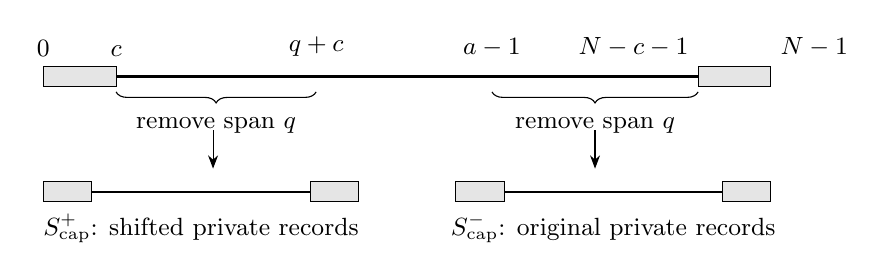
\begin{tikzpicture}[x=.77cm,y=.65cm,>=Stealth,font=\small]
 \draw[thick] (0,3)--(12,3);
 \draw[fill=gray!20] (0,2.8) rectangle (1.2,3.2);
 \draw[fill=gray!20] (10.8,2.8) rectangle (12,3.2);
 \node[above] at (0,3.2) {\(0\)}; \node[above] at (1.2,3.2) {\(c\)};
 \node[above] at (4.5,3.2) {\(q+c\)};
 \node[above] at (7.4,3.2) {\(a-1\)};
 \node[above,anchor=south east] at (10.8,3.2) {\(N-c-1\)};
 \node[above,anchor=south west] at (12,3.2) {\(N-1\)};
 \draw[decorate,decoration={brace,mirror,amplitude=4pt}] (1.2,2.7)--(4.5,2.7)
 node[midway,below=6pt] {remove span \(q\)};
 \draw[decorate,decoration={brace,mirror,amplitude=4pt}] (7.4,2.7)--(10.8,2.7)
 node[midway,below=6pt] {remove span \(q\)};
 \draw[->] (2.8,1.95)--(2.8,1.2); \draw[->] (9.1,1.95)--(9.1,1.2);
 \draw[thick] (0,.75)--(5.2,.75);
 \draw[fill=gray!20] (0,.55) rectangle (.8,.95);
 \draw[fill=gray!20] (4.4,.55) rectangle (5.2,.95);
 \node[below] at (2.6,.5) {\(\splus\): shifted private records};
 \draw[thick] (6.8,.75)--(12,.75);
 \draw[fill=gray!20] (6.8,.55) rectangle (7.6,.95);
 \draw[fill=gray!20] (11.2,.55) rectangle (12,.95);
 \node[below] at (9.4,.5) {\(\sminus\): original private records};
\end{tikzpicture}
\caption{The two singleton splices, shown schematically and not to scale.
Both preserve the full \((c+1)\)-caps.  Their private comparison is exactly
\(c<k<N-q-c\), so every pair \(k,k+q\in\mathcal I\) is represented.}
\label{fig:splices}
\end{figure}

\subsection{The complete weak return frames}

Write the source's full lists as \(X=(N,I)\) and \(Y=(C,0)\), so
\(I=X\setminus\{N\}\) and \(C=Y\setminus\{0\}\), in their original
decreasing orders.  In the cap calculations these letters denote proper
lists, not the competing outer.
In the relative index universe \(K=\{0,\ldots,c\}\) put
\[
 \begin{aligned}
 I_R&=(I\cap[a,m])-a,&C_R&=(C\cap[a,m])-a,\\
 I_L&=(I\cap[q,q+c])-q,&C_L&=(C\cap[q,q+c])-q,\\
 I_+&=(I\cap[N-c,N))- (N-c),&C_+&=(C\cap[N-c,N))-(N-c),\\
 I_-&=I\cap[1,c],&C_-&=C\cap[1,c].
 \end{aligned}
\]
The square matrices
\[
 B_R=\JT(I_R,C_R),\quad B_L=\JT(I_L,C_L),\quad
 G_R=\JT(I_+,C_+),\quad G_L=\JT(I_-,C_-)
\]
are actual weak proper blocks.  Their determinants are nonzero products of
connected component functions and unit pivots; their extreme inverse
entries may vanish.  Set \(U_{\mathrm{cap}}=\{c\}\cup I_+\) and \(V_{\mathrm{cap}}=\{0\}\cup C_-\).
The normalized upper and lower cap vectors are
\begin{equation}\label{eq:cap-polynomials}
 l(z)=\sum_{i\in U_{\mathrm{cap}}}\ell_i z^{c-i},\quad\ell_c=1,
 \qquad r(z)=\sum_{j\in V_{\mathrm{cap}}}r_jz^j,\quad r_0=1.
\end{equation}
Their full residuals are
\[
 v_L(j)=\sum_{i\in U_{\mathrm{cap}}}\ell_i h_{i-j},\qquad
 v_R(i)=\sum_{j\in V_{\mathrm{cap}}}h_{i-j}r_j.
\]
Thus \(v_L(j)=0\) for \(j\in C_+\), and \(v_R(i)=0\) for \(i\in I_-\),
by the actual upper-column and lower-row equations.
Put \(l_k=[z^k]l(z)\) and \(r_k=[z^k]r(z)\), with coefficients outside
\(0,\ldots,c\) equal to zero.  For ordered lists \(J,K\), the weighted
diagonal matrices are \(X_J=\diag(i)_{i\in J}\) and \(Y_K=\diag(j)_{j\in K}\),
with the entries in their original decreasing orders.
Every cap-vector coefficient on its actual support is nonzero: deleting any row
and the permanent bottom column, or the top row and any column, from a
connected cap leaves a feasible weak Jacobi--Trudi minor.  Its diagonal
matching cannot cancel.

The original period-\(p\) copies provide reference frames.
Write \(B_R^*=\JT(I_R^*,C_R^*)\) and \(B_L^*=\JT(I_L^*,C_L^*)\)
for their two complete reference lists.
In an actual ordinary-(a) row frame let \(w=d_pg+c\), \(\tau=t\)
and \(\sigma=s-d_pg\); then
\begin{equation}\label{eq:ordinary-references}
 B_R^*=\JT(U_{\mathrm{cap}}\setminus\{\sigma\},C_+),\qquad
 B_L^*=\JT(I_-,V_{\mathrm{cap}}\setminus\{\tau\}).
\end{equation}
For an ordinary-(a) column frame, set \(\sigma=t-d_pg\), \(\tau=s\).
The corresponding references are
\[
 B_R^*=\JT(U_{\mathrm{cap}},C_+\cup\{\sigma\}),\qquad
 B_L^*=\JT(I_-\cup\{\tau\},V_{\mathrm{cap}}).
\]
The added entries are genuinely absent from the respective cap lists.
In every reference formula \(\sigma\) is the upper active index and
\(\tau\) the lower active index.
For an ordinary period-\(d\) chart, its clock is the fixed signed
coefficient \(\lambda\) in the original annihilator
\(V_d-\lambda\delta_d\); the derivations are defined in
\Cref{sec:response}.  The column clock is therefore
\(-p(M-1)+s-t=-(N-p-c+\sigma-\tau)\).
For a mixed-(d) frame, let \(z_0\) be its initial corrected phase and \(o_0\)
its terminal deficient phase; put \(\tau=z_0\), \(\sigma=o_0-d_pg\).
Then
\[
 B_R^*=\JT(U_{\mathrm{cap}},C_+\cup\{\sigma\}),\qquad
 B_L^*=\JT(I_-,V_{\mathrm{cap}}\setminus\{\tau\}).
\]
These identities follow by comparing the cap's complete flag word with its
actual \(p\)-translate.  Nonexceptional bits agree; the two exceptional bits
are exactly the indicated deletion or addition.  The singleton endpoints
fix the \(0,c\) records.  Shared unit contacts are included.

Deleting all common betas from every return and reference leaves one
strict disjoint weak core \((I_0,C_0)\).  Its height jumps determine its two
lists, and the proper-height word is common to all internal \(g\)-bands.
Write \(A_0=\JT(I_0,C_0)\) for its complete matrix.
Consequently
\begin{equation}\label{eq:vacancy-template}
 (I_Z,C_Z)=(I_0\cup Z,C_0\cup Z),\qquad
 Z\subseteq\Omega:=K\setminus(I_0\cup C_0).
\end{equation}
Write \(Z_R=I_R\cap C_R\) and \(Z_L=I_L\cap C_L\) for the restored
common-beta sets of the right and left return frames.
These are not independently chosen masks.  The actual band sequence is
\(A\)-periodic; the references occupy residues \(0,d_p\) and the observed
returns residues \(B,d_p-B\) modulo \(A\).  Coincident residues carry the same
complete frames.  All zero-height buffers retain their actual triangular
inverse actions.


\section{The complete scalar and its second channel}\label{sec:response}

\subsection{The whole source gradient}
Let \(S\) be one original parent.  Put \(A_S=\JT(I,C)\), \(b=(h_i)_{i\in I}\), \(w=(h_{N-j})_{j\in C}\), and \(\kappa=\det A_S\).  Moving the distinguished column to the front gives the canonical Schur complement
\begin{equation}\label{eq:schur-complement}
 f_S=\frac{Q_S}{\kappa}=h_N-wA_S^{-1}b
       =\frac{s_S}{\partial_{h_N}s_S}.
\end{equation}
Equal original Schur functions therefore give the same normalized whole function.

Temporarily replace every physical \(h_0\) in every matrix by one variable \(\nu\), keep all negative entries zero, and put
\[
 \mathcal H(z)=\nu+\sum_{j>0}h_jz^j,\qquad \Theta_z=z\frac{d}{dz}.
\]
This is a coherent homogenization, not an additional observation: \(f_\nu(\boldsymbol h)=\nu f_1(\boldsymbol h/\nu)\).  Every observer below is homogeneous of ordinary degree one, so a whole identity at \(\nu=1\) extends exactly.  The operators fix \(\nu\).
For a rational function of \(\nu\), write \([\nu^k]_\infty\) for
its Laurent coefficient at infinity: substitute \(\nu=t^{-1}\),
expand at \(t=0\), and take the coefficient of \(t^{-k}\).

Differentiating \eqref{eq:schur-complement} gives the full gradient
\[
 \partial_{h_m}f_S=\one_{m=N}-w_mA_S^{-1}b
 -wA_S^{-1}b_m+wA_S^{-1}(A_S)_mA_S^{-1}b.
\]
In particular the inverse-motion term is present.  With the complete endpoint coframes
\[
 R_S(z)=1-\sum_{j\in C}(A_S^{-1}b)_jz^j,\qquad
 L_S(z)=1-\sum_{i\in I}(wA_S^{-1})_iz^{N-i},
\]
all occurrences of each repeated raw label collect to
\begin{equation}\label{eq:gradient-product}
 \partial_{h_m}f_S=[z^{N-m}]R_SL_S.
\end{equation}
Define the derivations
\[
 \delta_s=\sum_{j\ge s}h_{j-s}\partial_{h_j},\qquad
 V_s=\sum_{j\ge s}(j-s)h_{j-s}\partial_{h_j},\qquad
 \DD_s(\lambda)=V_s-\lambda\delta_s.
\]
The whole proper factor is below \(g\), so all operators at indices at least \(g\) fix it.  The genuine normalized observers at \(q\) are therefore
\begin{equation}\label{eq:whole-observers}
 O_H=[z^{m}]\mathcal HR_SL_S,\qquad
 O_\lambda=[z^{m}]\mathcal H(m-\lambda-\Theta_z)(R_SL_S).
\end{equation}
The original mixed chart supplies \(O_H=0\); an original ordinary chart supplies \(O_\lambda=0\) at its own fixed signed clock.  The term \(h_q\mapsto h_0\) creates \(\nu\), not zero.


For an ordinary case-(a) line chart with \(J\) cells and phase offset
\(\theta=s_f-t_f\), the clock is
\[
 \lambda=\eps q(J-1)+\theta,
 \qquad \eps=1\text{ for a row},\quad
        \eps=-1\text{ for a column}.
\]
Indeed composition covariance \cite[Composition covariance]{Shields2026Readout} acts on \(h_J\) or \(e_J\);
\(V_1h_J=(J-1)h_{J-1}\) and
\(V_1e_J=-(J-1)e_{J-1}\), while
\(\delta_1h_J=h_{J-1}\) and \(\delta_1e_J=e_{J-1}\).
The full local normalizer is fixed.  Whole antitransposition gives the
opposite ordinary reading with the rebuilt signed clock.  A mixed chart
instead supplies \(\delta_qQ_S=0\).  Thus each zero above is an identity
of the original whole function, not a presumed equality of the two
splices.

\subsection{Both actual return corrections}
Let \(R^0,L^0\) be the endpoint coframes of the actual first and last \(a\)-diagonal windows.  Their entries use labels below \(a\), and their heads through degree \(c\) are \(r,l\) of \eqref{eq:cap-polynomials}.  Define, for \(0\le i,j\le c\),
\begin{equation}\label{eq:base-residuals}
 P_i=[z^{a+i}]\mathcal HR^0,\qquad Q_j=[z^{m-j}]\mathcal H L^0,
 \qquad \rho=B_R^{-1}P_{I_R},\quad \zeta=Q_{C_L}^{t}B_L^{-1}.
\end{equation}
The full source systems give, through degree \(m\),
\begin{equation}\label{eq:source-truncations}
 R_S=R^0-\sum_{j\in C_R}\rho_jz^{a+j},\qquad
 L_S=L^0-\sum_{i\in I_L}\zeta_i z^{m-i}.
\end{equation}
Indeed the base equations are closed because every entry from a lower base row to a return column is a negative zero.  The remaining equations are exactly the two complete square systems in \eqref{eq:base-residuals}.  Their possible column \(m\) and row \(0\) are retained.  The product of the two correction tails has degree at least \(2a>m\), so contributes zero for a physical negative-slot reason.

Let
\begin{align*}
 u_L^0(j)&=\sum_{i\in U_{\mathrm{cap}}}(i-j)\ell_i h_{i-j},&
 u_R^0(i)&=\sum_{j\in V_{\mathrm{cap}}}(i-j)h_{i-j}r_j,\\
 x_R(z)&=\sum_{i\in I_R}(v_L(C_R)^tB_R^{-1})_iz^{c-i},&
 y_L(z)&=\sum_{j\in C_L}(B_L^{-1}v_R(I_L))_jz^j.
\end{align*}
Write \(x_R^0,y_L^0\) for the corresponding weighted projections obtained from \(u_L^0,u_R^0\).  Put
\[
 T_R=x_R/l,\qquad T_L=y_L/r\pmod {z^{c+1}},\qquad w_c=rl.
\]
The same \(c+1\) original variables \(h_a,\ldots,h_{a+c}\) occur at both ends.  In \(P_i\) their coefficients are \(r_{i-j}\); in \(Q_j\) they are \(l_{c-j-i}\).  Thus the entire shared-high coefficient polynomials are
\begin{equation}\label{eq:cap-high}
\begin{split}
 D(z)&=w_c-rx_R-ly_L=w_c(1-T_R-T_L),\\
 A(a,\lambda;z)&=(a+c-\lambda)w_c-\Theta_z w_c
 -r(x_R^0-\lambda x_R)-l(y_L^0-\lambda y_L),
\end{split}
\end{equation}
read modulo \(z^{c+1}\).  Each whole observer is equivalent to these \(c+1\) coefficient equations and one full remainder.  The denominators are low and independent of the high variables.  The residual vectors \(P,Q\) and the individual inverse entries are not independent probes.

\subsection{The full cap-functional identity}
Write \(f_E=f_{\sminus}\) and \(f_F=f_{\splus}\) for the normalized functions of the two actual cofaces.  For \(\langle T\rangle=[z^m]\mathcal H T\), their cross kernel \(K\) and balanced endpoint current \(J\) satisfy
\begin{equation}\label{eq:cap-duality}
 K=\langle R^0L^0\rangle,\qquad f_E=\langle R^0l\rangle,
 \qquad f_F=\langle L^0r\rangle,
\end{equation}
\begin{equation}\label{eq:paired-current}
 J=\langle\Theta_z(R^0L^0)-R^0\Theta_z l-L^0\Theta_z r\rangle.
\end{equation}
To prove \eqref{eq:cap-duality}, substitute the actual cap matrices \(G_R,G_L\) in \eqref{eq:source-truncations}; their cross corrections pair with \(v_L(C_+)=0\) and \(v_R(I_-)=0\).  The upper self-complement is
\[
 P_c-h_{c-C_+}G_R^{-1}P_{I_+}=\langle R^0l\rangle,
\]
and the lower formula is dual.  Differentiating the upper tail gives its index-weighted zero residual and the remaining \(\langle R^0\Theta_z l\rangle\) term; the lower one gives \(\langle L^0\Theta_z r\rangle\).  This proves \eqref{eq:paired-current} without a contact/endpoint alias.

For either observer set \((\eps_{\mathrm{obs}},s,C_1,D_1)=(0,1,x_R,y_L)\) in the Hall case, and
\[
 (\eps_{\mathrm{obs}},s,C_1,D_1)=
 (1,m-\lambda,x_R^0-\lambda x_R+\Theta_z l,
                  y_L^0-\lambda y_L+\Theta_z r)
\]
in the ordinary case.  Direct elimination gives
\[
 O=-\eps_{\mathrm{obs}} J+sK-\langle R^0C_1+L^0D_1\rangle.
\]
On the high equations, \(rC_1+lD_1=srl\pmod{z^{c+1}}\).  Since \(l(0)=r(0)=1\), define \(\gamma=(C_1/l)_{\le c}=\sum\gamma_kz^k\) and
\[
 T_k=\langle R^0(z^kl)_{\le c}-L^0(z^kr)_{\le c}\rangle.
\]
Then the exact whole identity is
\begin{equation}\label{eq:gamma-functional}
 O=-\eps_{\mathrm{obs}} J+\gamma_0(K-f_E)+(s-\gamma_0)(K-f_F)
                   -\sum_{k=1}^c\gamma_kT_k.
\end{equation}
There is no reason to discard the last sum from the high equations alone.  We will consume this same scalar by another exact representation, rather than require the \(T_k\) to be independent or \(\gamma_{k>0}\) to vanish.

\subsection{Coherent cap limits}
\begin{lemma}\label{lem:boolean}
For the actual source reference indices \(\sigma,\tau\), the entire truncated cap responses have
\[
\begin{aligned}
 T_R&\longrightarrow e_R\in\{0,1\},&
 x_R^0&\longrightarrow(c-\sigma)l_\infty-\Theta_z l_\infty,\\
 T_L&\longrightarrow e_L\in\{0,1\},&
 y_L^0&\longrightarrow\tau r_\infty-\Theta_z r_\infty
\end{aligned}
\]
as \(\nu\to\infty\).  In particular an ordinary high zero satisfies
\begin{equation}\label{eq:clock-infinity}
 \lambda(1-e_R-e_L)=a+\sigma-\tau>0.
\end{equation}
A Hall and an ordinary high zero cannot coexist on this same actual deck.
\end{lemma}
\begin{proof}
Delete paired units from the upper cap.  Its remaining rectangular lists \(J_0,K_0\) are disjoint with \(|J_0|=|K_0|+1\), \(c\in J_0\).  Its coframe limit \(\ell\) is normalized by \(\ell_c=1\) and satisfies \(\ell M(J_0,K_0)=0\).  Eliminating all other units leaves \(\nu I+E_Z\), with \(E_Z\) independent of \(\nu\).  Thus their coefficients are \(O(\nu^{-1})\) and the normalized limit is finite and nonzero by genuine cap weak cofactors.

There are two reference-core possibilities.  First, \(I_0=J_0\setminus\{\sigma\}\), \(C_0=K_0\), with \(\sigma\) a vacancy.  The residual on core columns is exactly zero; its only possible order-\(\nu\) vacancy entry is \(\nu\ell_\sigma\) at \(\sigma\).  If this vacancy is absent, the projected row tends to zero.  If present, the \(\nu^{-1}\) leading inverse and core back-substitution reconstruct \(\ell\), giving \(x_R\to l_\infty\).

Second, \(I_0=J_0\), \(C_0=K_0\cup\{\sigma\}\), with \(\sigma\) outside both rectangular lists.  If \(\sigma\) was a shared cap unit its own full residual is zero, and the projection tends to zero.  If it was absent from the cap columns, write \(\ell A_0=f e_\sigma^t\), \(f\ne0\); the projected row tends to \(\ell\).  This proves the Boolean limit without replacing a zero own-unit residual by absent forcing.

In the weighted projection an equal-slot coefficient is \(i-j=0\), so no order-\(\nu\) vacancy forcing survives.  In the first case the limiting row has entries \((i-\sigma)\ell_i\); in the second,
\[
 u_L^0(C_0)A_0^{-1}\longrightarrow
 \ell X_{J_0}-f e_\sigma^tY_{C_0}A_0^{-1}
 =\ell(X_{J_0}-\sigma I).
\]
Both give the upper weighted formula.  Transpose and reverse the finite index interval for the lower formula.  Empty cores and endpoint indices are included.  Dividing the ordinary equation in \eqref{eq:cap-high} by \(rl\) and taking these limits cancels both logarithmic derivatives and gives \eqref{eq:clock-infinity}.  A Hall zero would instead require \(e_R+e_L=1\).
\end{proof}

\subsection{The sum horizon and clock rigidity}
\begin{lemma}\label{lem:sum-horizon}
The block calculation \eqref{eq:source-truncations}--\eqref{eq:cap-high} applies at \(p+q\).  Its complete low cap and return data agree with those at \(q\), while its high variables are a different actual band.
\end{lemma}
\begin{proof}
Put \(a'=N-p-q-c\).  By \eqref{eq:horizon-bounds},
\[
 a'\ge |p-q|\ge g>c.
\]
The pins give the required singleton cuts, both correction tails begin at \(a'\), their product is beyond \(a'+c\), and the base labels are below \(a'\).  These are exactly the block proof's requirements.  No period-\((p+q)\) chart or stronger coface bound \(N-p-q\ge2g\) is used.

The two left bands are \([q,q+c]\) and \([p+q,p+q+c]\); the right bands are \([a'+p,a'+p+c]\) and \([a',a'+c]\).  All positions lie in the original open periodic interval.  Original \(p\)-periodicity equates the full low frames.  The end caps are unchanged.  Each horizon separately has one shared high vector, but the two high vectors are not identified.
\end{proof}

The actual clocks are fixed integers.  Direct calculation on every generator, including the equality case that creates \(\nu\), gives
\[
\begin{split}
 [\DD_p(\alpha),\DD_q(\beta)]
  &=(p-q)V_{p+q}+(q\beta-p\alpha)\delta_{p+q},\\
 [\delta_p,\DD_q(\beta)]&=p\delta_{p+q}.
\end{split}
\]
For \(h_j\) with \(j=p+q+k\), the first coefficient is
\[
 (k+p-\beta)(k-\alpha)-(k+q-\alpha)(k-\beta)
 =(p-q)k+q\beta-p\alpha.
\]
Below the sum both compositions vanish.  These annihilator consequences use the two original whole identities on one \(f_S\), not merely their high coefficients.

\begin{proposition}[Type and clock compatibility]\label{prop:clocks}
Mixed/ordinary comparisons do not occur in \eqref{eq:hard-domain}.  In an ordinary/ordinary comparison the clocks have a common sign \(\eps\) and a common cap defect \(\Delta\in[0,2c]\):
\[
 \alpha=\eps(N-p-\Delta),\qquad
 \beta=\eps(N-q-\Delta),\qquad D(z)=\eps r(z)l(z).
\]
After lawful whole positive-clock normalization,
\begin{equation}\label{eq:complementary}
 \lambda=a+\sigma-\tau,\qquad T_R+T_L=0.
\end{equation}
For mixed/mixed charts the genuine relation is \(T_R+T_L=1\).
\end{proposition}
\begin{proof}
A mixed source and ordinary mate have \(\delta_pf=0\) and \(\DD_q(\beta)f=0\).  Their commutator gives \(\delta_{p+q}f=0\).  By \Cref{lem:sum-horizon} the same \(q\)-deck has both a Hall and an ordinary high zero, contrary to \Cref{lem:boolean}.  Interchange parents for the reverse ordered case.

For ordinary charts, use \(\sigma\) for the upper active index and \(\tau\) for the lower active index in both reference types.  In a physical source case-(a) frame write \(\alpha=\eps d_p\) with \(d_p=N-p-c+\sigma-\tau>0\).  The weighted cap limit gives \(\beta=\eta d_q\), \(d_q=N-q-c+\sigma-\tau>0\), and \(D/(rl)\to\eta\).  The whole commutator gives a sum-horizon clock
\[
 \gamma=\frac{p\alpha-q\beta}{p-q}.
\]
Subtract its high equation from the \(q\) equation, whose low data are equal by \Cref{lem:sum-horizon}.  Since \(a'=a-p\),
\[
 0=-p\,rl-(\gamma-\beta)D,
 \qquad (\alpha-\beta)D=(q-p)rl.
\]
The clocks cannot be equal.  At coherent unit infinity the second identity gives \(\alpha=\eta d_p\), hence \(\eta=\eps\).  The full identity then gives \(D=\eps rl\).  Take \(\Delta=c-\sigma+\tau\).

For a negative clock, antitranspose the entire original comparison.  On full flags this sends \((X,Y)\) to \(([0,N]\setminus Y,[0,N]\setminus X)\), and on a return band \((I,C)\) to \((K\setminus C,K\setminus I)\) for \(K=\{0,\ldots,c\}\).  Consequently a genuine completion reference becomes a deletion reference at an actual transformed cap index.  Rebuild all frames and rehomogenize.  The physical involution reverses the clock sign, proving \eqref{eq:complementary} with actual deletion references \eqref{eq:ordinary-references}.  The mixed relation is its original Hall high equation.  No whole Hall zero has been added to the ordinary case.
\end{proof}


\section{Endpoint poles and outward boundary defects}\label{sec:poles}

The complementary response will be used only to remove the defects that could spoil a sign argument.  The complete scalar remains to be consumed afterward.  Throughout this section every true unit is the same \(\nu\).

For the comparison statements here and in \Cref{sec:whole-sign},
retain \eqref{eq:hard-domain}, the actual cap-preserving splices,
the full cap and reference lists of \Cref{sec:geometry}, and the common
weak core and coupled returns of \eqref{eq:vacancy-template}.
In the ordinary case use the whole positive-clock normalization of
\Cref{prop:clocks}.  The return sets remain observed bands of the
same periodic source, not independently chosen masks.
The input to \Cref{thm:end-filter} is the complementary response:
\eqref{eq:complementary} in the ordinary case and \(T_R+T_L=1\)
in the mixed case.  \Cref{thm:scalar-synchronization} additionally uses
the original complete ordinary or Hall zero in
\eqref{eq:whole-observers}; no independent scalar zero is assigned to
either coface.

\subsection{Weak Jacobi--Trudi signs}
\begin{lemma}[Simultaneous negative-lex sign]\label{lem:weak-sign}
For this sign specialization fix a positive real value of \(h_0=\nu\),
including the physical value \(\nu=1\).
Let \(X_1>\cdots>X_m\), \(Y_1>\cdots>Y_m\) satisfy \(X_i\ge Y_i\).  The weak determinant is nonzero.  In lexicographic order \(h_M\gg h_{M-1}\gg\cdots\gg h_1\), its leading monomial, evaluated with all positive generators negative, has sign
\[
 (-1)^{\eta(X,Y)},\qquad
 \eta(X,Y)=\#\{(i,j):i\ge j,\ X_i>Y_j\}.
\]
For every finite collection of such determinants, one specialization realizes all these signs simultaneously, with all denominators nonzero.
\end{lemma}
\begin{proof}
For nonvanishing, the diagonal matching is supported.  Its squared-index cost \(\sum_i(X_i-Y_i)^2\) is uniquely smallest among permutations by strict rearrangement.  A determinant monomial records its positive indices and, at fixed matrix size, the number of zeros.  No other supported permutation therefore has that diagonal monomial.

Induct on \(m\) for the sign.  If \(X_k=Y_k\), the actual unit pivot and its surrounding triangular zeros split the determinant into the weak upper-left and lower-right blocks.  The exponent \(\eta\) adds.  If \(X_{k+1}<Y_k\), a negative-zero lower-left block gives the same factorization.  Otherwise the positive block is connected.  Its largest label \(X_1-Y_m\) occurs only at the top-right entry and has a nonzero feasible proper cofactor.  The lex-leading term uses that entry.  Its sorting sign is \((-1)^{m-1}\) and the negative generator adds one minus sign, giving \((-1)^m\).  The full exponent is \(m\) plus the proper-cofactor exponent, completing the induction.  Empty determinants have sign one.

For simultaneity, let \(B\) exceed twice the largest matrix size plus two and set \(h_j=-T^{B^j}\).  The exponent of \(T\) realizes lex order for all their bounded-degree monomials.  For one sufficiently large positive \(T\), every leading term dominates and all asserted signs hold.  Apply this to the finite union of all numerators and denominators required in the argument.
\end{proof}

\subsection{Actual masks and cap-height placement}
Let \(A_0=\JT(I_0,C_0)\) be the common disjoint weak return core in \eqref{eq:vacancy-template}.  It may be empty or disconnected.  Its height is
\[
 h_D(u)=\#\{i\in I_0:i>u\}-\#\{j\in C_0:j>u\}\ge0.
\]
The actual reference equations imply
\begin{equation}\label{eq:reference-differences}
 \one_{I_R^*}-\one_{C_R^*}=\one_{U_{\mathrm{cap}}}-\one_{C_+}-\one_\sigma,
 \qquad
 \one_{C_L^*}-\one_{I_L^*}=\one_{V_{\mathrm{cap}}}-\one_{I_-}-\one_\tau.
\end{equation}
Thus \(\sigma\) is either a vacancy or a core column, and \(\tau\) a vacancy or a core row.  Away from the active index, the two cap memberships at a vacancy agree.  Denote their paired sets by
\[
 S_R=(U_{\mathrm{cap}}\cap C_+)\cap\Omega\setminus\{\sigma\},\qquad
 S_L=(I_-\cap V_{\mathrm{cap}})\cap\Omega\setminus\{\tau\}.
\]
The Boolean limits have the following exact meaning.  If \(\sigma\) is a vacancy, the cap contains its row but not its column, and \(e_R=\one_{\sigma\in Z_R}\).  If \(\sigma\in C_0\), the cap contains both row and column when \(e_R=0\), and neither when \(e_R=1\).  The lower alternatives are dual.  These exhaust the binary possibilities in \eqref{eq:reference-differences}.

Define
\[
\begin{split}
 A_R&=
 \begin{cases}(Z_R\setminus S_R)\setminus\{\sigma\},&e_R=0,\\
 S_R\setminus Z_R,&e_R=1,
 \end{cases}\\
 A_L&=
 \begin{cases}(Z_L\setminus S_L)\setminus\{\tau\},&e_L=0,\\
 S_L\setminus Z_L,&e_L=1.
 \end{cases}
\end{split}
\]
They are added units when \(e=0\) and missing cap units when \(e=1\), never the active anchor itself.  The actual cap heights are
\begin{equation}\label{eq:cap-height-pole}
 H_{\rm upper}(u)=1+h_D(u)-\one_{u\ge\sigma},\qquad
 H_{\rm lower}(u)=1+h_D(u)-\one_{u<\tau}.
\end{equation}
For the upper cap the distinguished bottom column is at \(-1\); its top is \(c\).  The lower cap runs from \(0\) to the top at \(c+1\).  Hence connectedness gives
\begin{equation}\label{eq:cap-height-positive}
 h_D(u)\ge1\quad(\sigma\le u<c),\qquad
 h_D(u)\ge1\quad(0\le u<\tau).
\end{equation}
If \(\sigma<c\), the highest positive core component has support \([b,c)\) with \(b\le\sigma\), and every vacancy above \(\sigma\) lies in this one component.  If \(\tau>0\), the lowest component has support \([0,d)\) with \(\tau\le d\).  At \(\sigma=c\) or \(\tau=0\) the corresponding outward interval is empty.  The two components may coincide or have equal functions; no connected full-span return core is assumed.

\subsection{The first complete projection defect}
Let \(\ell^\infty,r^\infty\) be the cap limits.  For an absent nonactive vacancy define the limiting off-diagonal forcing
\[
 G_u=\sum_i\ell_i^\infty h_{i-u},\qquad
 F_u=\sum_jh_{u-j}r_j^\infty.
\]
These are not the full residuals at an own inserted unit.  Such a unit satisfies
\begin{equation}\label{eq:own-unit}
 0=\nu\ell_u+\sum_{i\ne u}\ell_i h_{i-u},\qquad
 \ell_u=-\nu^{-1}G_u+O(\nu^{-2}),
\end{equation}
and dually \(r_u=-\nu^{-1}F_u+O(\nu^{-2})\).  This derives its coefficient independently of its zero full residual.

Set
\[
\begin{split}
 \phi_u(z)&=z^{c-u}-M(u,C_0)A_0^{-1}(z^{c-i})_{i\in I_0},\\
 \psi_u(z)&=z^u-(z^j)_{j\in C_0}A_0^{-1}M(I_0,u).
\end{split}
\]
Here \(M(R,C)=(h_{r-c})\) on the indicated actual lists.  Empty matrices have their empty action.

\begin{lemma}\label{lem:first-response}
Coefficientwise through degree \(c\),
\begin{equation}\label{eq:first-response}
 T_R=e_R+\nu^{-1}\sum_{u\in A_R}\frac{G_u\phi_u}{l_\infty}+O(\nu^{-2}),
 \qquad
 T_L=e_L+\nu^{-1}\sum_{u\in A_L}\frac{F_u\psi_u}{r_\infty}+O(\nu^{-2}).
\end{equation}
\end{lemma}
\begin{proof}
For \(e_R=0\), all core columns are actual cap columns, so their full residual is exactly zero.  Eliminate the whole disjoint core in the actual return matrix.  Its vacancy complement is
\begin{equation}\label{eq:vacancy-resolvent}
 \nu I_Z+E[Z,Z],\qquad
 E_{uv}=h^+_{u-v}-M(u,C_0)A_0^{-1}M(I_0,v),
\end{equation}
where \(h^+_j=h_j\) for \(j>0\) and zero otherwise.  The inverse begins with \(\nu^{-1}I\).  Cap units have zero full residual; added nonactive vacancies have leading forcing \(G_u\).  Core back-substitution gives \(\phi_u\), proving the upper addition formula.

For \(e_R=1\), the active row is included in the return, or absent from the cap as well.  The only missing cap rows are \(S_R\setminus Z_R\).  Exact full row representation gives
\[
 x_R-l=-\sum_{u\in S_R\setminus Z_R}\ell_u\phi_u^{B_R},
\]
where the superscript means the complete actual return inverse.  A missing vacancy has no equal core/cross index, so \(\phi_u^{B_R}\to\phi_u\).  Substitute \eqref{eq:own-unit}; the two minus signs give the same plus sign in \eqref{eq:first-response}.  The lower proof is the actual column dual.  All feedback in \eqref{eq:vacancy-resolvent} is retained before taking this coefficient.
\end{proof}

\subsection{Local connected components and their endpoint products}
For the upper extreme component with absolute support \([b,c)\), the
local indices corresponding to the band indices \(z,\sigma\) are
\(z-b,\sigma-b\), and its span is \(s=c-b\).  Translating every row
and column label by \(-b\) preserves every difference and hence every
matrix entry.  The lower extreme component already has lower endpoint
zero.  The formulas in this subsection use these local indices; the
endpoint filter below returns to the original band coordinates.

Normalize an actual connected disjoint component to full flags
\((s,I)/(C,0)\), and write \(D=\JT((s,I),(C,0))\) for its whole matrix.
Put
\begin{equation}\label{eq:local-pole-data}
\begin{split}
 K&=\JT(I,C),\quad b=h_I,\quad a_0=h_{s-C},\\
 F_D&=h_s-a_0K^{-1}b=h_s-\omega_D,\\
 f_z&=h_z-M(z,C)K^{-1}b,\qquad
 g_z=h_{s-z}-a_0K^{-1}M(I,z),\quad P_z=f_zg_z.
\end{split}
\end{equation}
All \(f_z,g_z,\omega_D\) use indices below \(s\).  Solving the proper columns first and then the bottom column gives the exact top-row projection
\[
 M(z,\text{full columns})D^{-1}e_{\rm top}=f_z/F_D.
\]
This is a complete inverse identity, not replacement of the frame by its determinant.

\begin{lemma}\label{lem:local-forcing}
For the upper cap restricted to this component,
\begin{equation}\label{eq:cap-pole-regular}
 G_z=g_z-F_DU_z,\qquad U_z\in\Q(h_1,\ldots,h_{s-1}).
\end{equation}
Dually \(F_z=f_z-F_DV_z\) with \(V_z\) in the same lower field.  At one simultaneous negative-lex specialization, every \(P_z\) at an actual interior vacancy is strictly positive, including products from different connected components.
\end{lemma}
\begin{proof}
Define \(k(u,z)=h_{u-z}-M(u,C)K^{-1}M(I,z)\).  Every upper anchor case has an explicit correction:
\[
 U_z=\begin{cases}
 0,&\sigma=0\text{ is the bottom core column},\\
 k(\sigma,z)/f_\sigma,&\sigma\text{ is a vacancy},\\
 \dfrac{e_\sigma^tK^{-1}M(I,z)}{e_\sigma^tK^{-1}b},
 &\sigma\text{ is a proper core column}.
 \end{cases}
\]
Start with the endpoint-left vector \((1,-a_0K^{-1})\).  At a fresh row \(\sigma\) its correction coefficient is \(-F_D/f_\sigma\), giving the middle formula.  At a shared core-column unit its own coefficient is \(O(\nu^{-1})\), and the remaining limiting vector is corrected by \(-F_D e_\sigma^tK^{-1}/(e_\sigma^tK^{-1}b)\).  Removing that column gives the same limiting equations.  The bottom-column case is the endpoint vector.  This proves \eqref{eq:cap-pole-regular}.  The displayed denominators are nonzero actual weak Cramer coefficients and omit \(h_s\).

For the lower side, \(V_z=0\) at the top core row, \(V_z=k(z,\tau)/g_\tau\) at a fresh vacancy, and
\[
 V_z=\frac{M(z,C)K^{-1}e_\tau}{a_0K^{-1}e_\tau}
\]
at a proper core-row anchor.  The same complete solve proves these formulas and their nonzero denominators.

The numerators of \(f_z,g_z\) are, with their actual Cramer sorting signs, the weak boards
\[
 (I\cup\{z\})/(C\cup\{0\}),\qquad
 (I\cup\{s\})/(C\cup\{z\}).
\]
Their heights are the component height lowered by one on \([z,s)\) and \([0,z)\), respectively.  They are feasible and nonzero.  To compute the product sign, put \(n_I(x)=\#\{i\in I:i>x\}\) and \(n_C(x)=\#\{j\in C:j<x\}\).  Counting positive entries and the two insertion permutations in \Cref{lem:weak-sign} gives the normalized product sign
\[
 (-1)^{n_I(0)+n_I(s)+n_C(0)+n_C(s)}=(-1)^{|I|+|C|}=+1.
\]
The denominator is \(\det K^2\).  This parity is positive across components, not just a common unspecified sign within one contact pair.  Apply the simultaneous specialization to the finite union of all these weak numerators, denominators, cap normalizers, and shifted source matrices used below.
\end{proof}

\subsection{The endpoint filter, including equal poles}
Let \(t_R=[z^0]T_R\) and \(t_L=[z^0]T_L\).  If the highest component has support \([b,c)\) and span \(s_R=c-b\), then \(A_0^{-1}e_c\) is supported on that component.  Rows below \(b\) are negative against its columns.  The upper cap equations on those high columns are closed.
In band coordinates, \(P_u^{D_R}\) denotes the local product \(P_{u-b}\)
computed after subtracting \(b\) from the upper component's row and column
labels; \(P_u^{D_L}\) uses the unchanged lower coordinate \(u\).
By \Cref{lem:first-response,lem:local-forcing},
\begin{equation}\label{eq:end-pole-expansion}
\begin{aligned}
 [\nu^{-1}]_\infty t_R&=-\frac{S_R^{\rm end}}{F_{D_R}}+R_R,
 &S_R^{\rm end}&=\sum_{u\in A_R\cap(b,c)}P_u^{D_R},\\
 [\nu^{-1}]_\infty t_L&=-\frac{S_L^{\rm end}}{F_{D_L}}+R_L,
 &S_L^{\rm end}&=\sum_{u\in A_L\cap(0,d)}P_u^{D_L}.
\end{aligned}
\end{equation}
With superscripts specifying the normalized components, the regular
terms in the same local coordinates are
\[
 R_R=\sum_{u\in A_R\cap(b,c)}
       f^{D_R}_{u-b}U^{D_R}_{u-b},\qquad
 R_L=\sum_{u\in A_L\cap(0,d)}
       g^{D_L}_uV^{D_L}_u.
\]
Indeed the full endpoint summands are
\[
 -\frac{G_zf_z}{F_D}
   =-\frac{f_zg_z}{F_D}+U_zf_z,\qquad
 -\frac{F_zg_z}{F_D}
   =-\frac{f_zg_z}{F_D}+V_zg_z.
\]
The upper expression uses \(z=u-b\) and the component's top-row
normalization; the lower one uses \(z=u\) and its bottom-column
normalization.  Thus each regular sum has the same indexing set as
its pole numerator.
Each regular term uses only labels strictly below the span of its own end component.  The two formulas include all intermediate weak components and unit buffers; they disappear from these particular coefficients only by the proved triangular support.  If an outward endpoint interval is empty, that end contribution is zero.

\begin{theorem}[End-pole filter]\label{thm:end-filter}
Under the ordinary or mixed complementary response,
\begin{equation}\label{eq:outward-filter}
 A_R\cap(\sigma,c]=\varnothing,\qquad
 A_L\cap[0,\tau)=\varnothing.
\end{equation}
In fact each discrepancy set misses the interior of its corresponding
active extreme positive component just defined: the upper component when
\(\sigma<c\), and the lower component when \(\tau>0\).
\end{theorem}
\begin{proof}
By \Cref{prop:clocks}, \(t_R+t_L\) is the constant zero or one, so its \(\nu^{-1}\) coefficient is zero.  Choose the larger end-component span \(s\).  Regard \(h_s\) as independent over \(\Q(h_1,\ldots,h_{s-1})\).  Terms from a smaller-span end and the regular terms at span \(s\) are independent of \(h_s\).  Each span-\(s\) denominator is the monic linear factor \(h_s-\omega_D\).

If the two factors differ, separate residues make each corresponding \(S^{\rm end}\) zero.  If they coincide, the residue is \(-(S_R^{\rm end}+S_L^{\rm end})\).  By \Cref{lem:local-forcing} every nonempty summand has a simultaneous strictly positive specialization, so this sum cannot vanish unless both indexing sets are empty.  Once a set is empty, its entire contribution in \eqref{eq:end-pole-expansion}, including the regular part, disappears because it was a sum over that set.  Treat the smaller end in the remaining exact equation.  This proves the stronger end-component exclusion; \eqref{eq:cap-height-positive} implies \eqref{eq:outward-filter}.

The sign test on a residue numerator uses the lower-index restriction of the one chosen specialization.  It does not evaluate the original scalar at a pole.  Equal factors do not identify inverse frames or erase their occurrence multiplicities.
\end{proof}

\Cref{fig:end-poles} shows the two extreme components and the excluded outward intervals.

\begin{figure}[t]
\centering
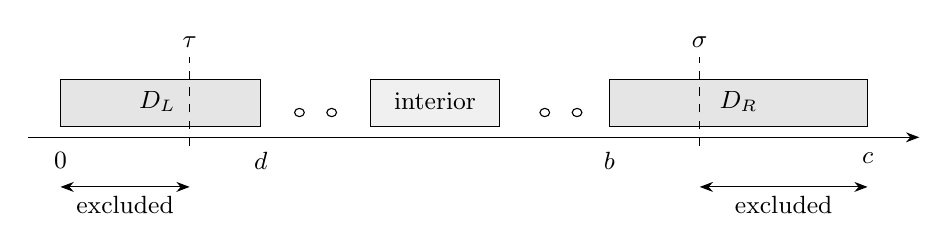
\begin{tikzpicture}[x=.82cm,y=.7cm,>=Stealth,font=\small]
 \draw[->] (0,0)--(13.8,0);
 \fill[gray!20] (.5,.2) rectangle (3.6,1.05);
 \fill[gray!12] (5.3,.2) rectangle (7.3,1.05);
 \fill[gray!20] (9,.2) rectangle (13,1.05);
 \draw (.5,.2) rectangle (3.6,1.05);\draw (5.3,.2) rectangle (7.3,1.05);\draw (9,.2) rectangle (13,1.05);
 \node at (2,.65) {\(D_L\)};\node at (6.3,.65) {interior};\node at (11,.65) {\(D_R\)};
 \foreach \x in {4.2,4.7,8.0,8.5}{\draw (\x,.45) circle (.075);}
 \draw[dashed] (2.5,-.15)--(2.5,1.45);\draw[dashed] (10.4,-.15)--(10.4,1.45);
 \node[above] at (2.5,1.45) {\(\tau\)};\node[above] at (10.4,1.45) {\(\sigma\)};
 \node[below] at (.5,-.1) {\(0\)};\node[below] at (3.6,-.1) {\(d\)};
 \node[below] at (9,-.1) {\(b\)};\node[below] at (13,-.1) {\(c\)};
 \draw[<->] (.5,-.9)--(2.5,-.9) node[midway,below] {excluded};
 \draw[<->] (10.4,-.9)--(13,-.9) node[midway,below] {excluded};
\end{tikzpicture}
\caption{The cap heights place outward discrepancies inside the two extreme positive components.  Unit buffers and intermediate feedback remain.  When the two end factors agree, their specific endpoint residues add with the same sign.}\label{fig:end-poles}
\end{figure}

\begin{example}\label{ex:c3}
For \(I_0=\{3\}\), \(C_0=\{0\}\) and vacancies \(1,2\), the return frames are
\[
 [h_3],\quad
 \begin{pmatrix}h_2&h_3\\\nu&h_1\end{pmatrix},\quad
 \begin{pmatrix}h_1&h_3\\\nu&h_2\end{pmatrix},\quad
 \begin{pmatrix}h_1&h_2&h_3\\\nu&h_1&h_2\\0&\nu&h_1\end{pmatrix}.
\]
The middle determinants are both \(h_1h_2-\nu h_3\), but their labeled inverses differ.  The component has \(F_D=h_3\) and both endpoint products equal \(h_1h_2\).  Its endpoint pole is therefore
\[
 -\bigl(|A_R|+|A_L|\bigr)h_1h_2/h_3.
\]
It cannot cancel.  The full observer, not this coefficient alone, must still determine the private records.  This is a symbolic interface illustration, not a supplied original pair with two minimum charts.
\end{example}


\section{Whole-determinant noncancellation}\label{sec:whole-sign}

Return to the physical value \(\nu=1\).  Every term of
\eqref{eq:gamma-functional}, including its nonconstant low-coefficient
cap-mode sum, remains present.  The pole filter has not classified
all rational response germs.  The same original scalar has a representation
that no longer requires such a classification.

For \(x\in X\), let \(\mathcal R_x\) be the determinant in the \emph{original
row order} after replacing the row label \(x\) by \(x-q\).  For \(y\in Y\), let
\(\mathcal C_y\) be the determinant in the original column order after
replacing \(y\) by \(y+q\).  For the original source, duplicate rows or
columns and negative or out-of-horizon replacements give zero.  Every
remaining entry is the actual shared raw moment; no individual term is
observed separately.

\begin{lemma}\label{lem:shifted-gradient}
For any equal-length strict integer lists \(X,Y\) and positive integer
\(q\), let \(s_S=\det\JT(X,Y)\) and take \(\mathcal R_x,\mathcal C_y\)
to be the literal replacement determinants in the original orders.
Then the following Hall and weighted identities hold without
connectedness or the original comparison hypotheses:
\begin{equation}\label{eq:shifted-gradient}
 \delta_q s_S=\sum_{x\in X}\mathcal R_x
             =\sum_{y\in Y}\mathcal C_y,\qquad
 V_qs_S=\sum_{x\in X}(x-q)\mathcal R_x
                   -\sum_{y\in Y}y\mathcal C_y.
\end{equation}
In the original comparison, the genuine positive ordinary clock
\(\lambda=r_*-\tau\), \(r_*=a+\sigma\), gives the specialization
\begin{equation}\label{eq:whole-shift}
 \DD_q(\lambda)s_S
 =\sum_{x\in X}(x-q-r_*)\mathcal R_x
      +\sum_{y\in Y}(\tau-y)\mathcal C_y.
\end{equation}
\end{lemma}
\begin{proof}
Differentiate the determinant by every entry occurrence.  Replacing the
whole row \(x\) gives the derivative contribution with entry
\(h_{x-y-q}\); summing the rows is the Hall derivative.  The same argument
by columns gives its second expansion.  For the weighted derivative,
\(x-y-q=(x-q)-y\), which gives the two terms in
\eqref{eq:shifted-gradient}.  At \(x-y=q\), the two weighted contributions
cancel while the Hall contribution retains \(h_0=1\).
For the empty matrix, the determinant is one and both derivatives and
all replacement sums are zero.  In the original clock setting, split
the single coefficient \(\lambda=r_*-\tau\) between the two equal
Hall expansions to obtain \eqref{eq:whole-shift}.  This splitting does not
assert a Hall zero in the ordinary case.
\end{proof}

For the original connected source, \(\kappa(S)\) is fixed and nonzero.
Thus the zero of \eqref{eq:whole-shift} is precisely the original ordinary
zero \eqref{eq:whole-observers}, up to its fixed nonzero normalization.
The mixed zero is either full Hall sum in \eqref{eq:shifted-gradient}.
Thus no cap-mode remainder has been omitted in changing representations.

\subsection{Feasibility and signs in the original orders}

\begin{lemma}\label{lem:shift-sign}
For the original connected source, every nonduplicate in-horizon shift
above is a nonzero weak Jacobi--Trudi determinant.  Relative to the
reference sign \((-1)^{\eta(X,Y)}\) at one
simultaneous specialization of \Cref{lem:weak-sign}, with \(w_0=x-q\)
and \(v_0=y+q\),
\begin{equation}\label{eq:shift-sign}
 \begin{aligned}
 \frac{\operatorname{sign}\mathcal R_x}{(-1)^{\eta(X,Y)}}
 &=(-1)^{\#(X\cap(w_0,x))+\#(Y\cap[w_0,x))}\\
 &=(-1)^{H_S(w_0)-H_S(x-1)+\one_{w_0\in Y}},\\
 \frac{\operatorname{sign}\mathcal C_y}{(-1)^{\eta(X,Y)}}
 &=(-1)^{\#(Y\cap(y,v_0))+\#(X\cap(y,v_0])}\\
 &=(-1)^{H_S(y)-H_S(v_0-1)+\one_{v_0\in X}}.
 \end{aligned}
\end{equation}
\end{lemma}
\begin{proof}
Lowering a row from \(x\) to \(w_0\ge0\) subtracts one from the positive
source height on \([w_0,x)\).  Raising a column from \(y\) to \(v_0\le N\)
subtracts one on \([y,v_0)\).  Thus the new sorted lists are weakly feasible,
even if the resulting diagram is disconnected or has diagonal units.
\Cref{lem:weak-sign} proves nonvanishing.

Sorting the changed row contributes \(\#(X\cap(w_0,x))\) swaps.  Its
positive-entry count changes by \(-\#(Y\cap[w_0,x))\).  For a feasible
\(r\)-row weak matrix, every entry strictly above the diagonal is positive,
so \(\eta\) is the positive-entry count minus \(r(r-1)/2\).  This proves the
first row formula; the column proof is the same.  Cumulative counts give
the displayed height forms modulo two.  Apply \Cref{lem:weak-sign} to the
finite collection of all surviving shifted matrices at once.
\end{proof}

For \(c<k<a\), \(k\) and \(k+q\) lie in the original open middle.  Their adjacent
heights agree by \(\mathcal P(g,c)\), using the actual pins at the first
boundary.  A surviving row shift \(k+q\to k\) is a unit at \(k+q\) and a
vacancy at \(k\); a surviving column shift is the reverse discrepancy.
Both have relative sign \(+1\).  Their ordinary coefficients are
\begin{equation}\label{eq:private-weights}
 k-r_*<0,\qquad \tau-k<0.
\end{equation}

The full cap ledger in \Cref{tab:cap-signs} follows by substituting
\eqref{eq:cap-height-pole} in \eqref{eq:shift-sign}.  The variable \(v\) in the table is a nonactive
relative cap vacancy.
For example, a missing nonactive upper cap unit at \(v\) has source
row \(x=N-c+v\) and returned position \(x-q=a+v\), absent from both
returned lists.  Since \(v\) is a core vacancy,
\(h_D(v-1)=h_D(v)\).  The actual heights give
\[
 H_S(a+v)=1+h_D(v),\qquad
 H_S(N-c+v-1)=1+h_D(v)-\one_{v>\sigma}.
\]
Also \(\one_{a+v\in Y}=0\).
The row formula in \eqref{eq:shift-sign} gives relative sign
\((-1)^{\one_{v>\sigma}}\); its ordinary coefficient is
\(v-\sigma\).  Their product is negative on either side of \(\sigma\).
\begin{table}[ht]
\centering\small
\begin{tabular}{@{}llll@{}}
\toprule
Shift & Actual discrepancy & Relative sign & Ordinary coefficient\\
\midrule
Row, \(x-q=v\) & added lower unit & \(-\) if \(v<\tau\); \(+\) if \(v>\tau\) & \(v-r_*\)\\
Row, \(x-q=a+v\) & missing upper unit & \(+\) if \(v<\sigma\); \(-\) if \(v>\sigma\) & \(v-\sigma\)\\
Column, \(y=v\) & missing lower unit & \(-\) if \(v<\tau\); \(+\) if \(v>\tau\) & \(\tau-v\)\\
Column, \(y=a+v\) & added upper unit & \(+\) if \(v<\sigma\); \(-\) if \(v>\sigma\) & \(\tau-a-v\)\\
\bottomrule
\end{tabular}
\par\medskip
\caption{Signs in the original matrix orders, relative to the same
reference sign.  The only potentially wrong-sign weighted additions are
exactly the outward records removed by \Cref{thm:end-filter}.}
\label{tab:cap-signs}
\end{table}

The active positions follow from the binary membership alternatives
in \eqref{eq:reference-differences}.  In the upper rows below, the cap
and return pairs are
\((\one_{U_{\mathrm{cap}}}(\sigma),\one_{C_+}(\sigma))\) and
\((\one_{I_R}(\sigma),\one_{C_R}(\sigma))\);
the shifts are \(\mathcal R_{N-c+\sigma},\mathcal C_{a+\sigma}\).
In the lower rows the pairs are
\((\one_{I_-}(\tau),\one_{V_{\mathrm{cap}}}(\tau))\) and
\((\one_{I_L}(\tau),\one_{C_L}(\tau))\);
the shifts are \(\mathcal R_{q+\tau},\mathcal C_\tau\).

{\small\centering
\begin{tabular}{@{}llcccc@{}}
\toprule
Anchor & Boolean value & Cap pair & Return pair & Row term & Column term\\
\midrule
Upper vacancy & \(e_R=0\) & \((1,0)\) & \((0,0)\) & live, weight \(0\) & absent\\
Upper core column & \(e_R=0\) & \((1,1)\) & \((0,1)\) & live, weight \(0\) & duplicate\\
Upper vacancy & \(e_R=1\) & \((1,0)\) & \((1,1)\) & duplicate & live\\
Upper core column & \(e_R=1\) & \((0,0)\) & \((0,1)\) & absent & live\\
\midrule
Lower vacancy & \(e_L=0\) & \((0,1)\) & \((0,0)\) & absent & live, weight \(0\)\\
Lower core row & \(e_L=0\) & \((1,1)\) & \((1,0)\) & duplicate & live, weight \(0\)\\
Lower vacancy & \(e_L=1\) & \((0,1)\) & \((1,1)\) & live & duplicate\\
Lower core row & \(e_L=1\) & \((0,0)\) & \((1,0)\) & live & absent\\
\bottomrule
\end{tabular}\par}

For ordinary state \(00\), every live active term has zero weight.
For mixed state \(10\), the row Hall expansion has only absent or
duplicate active row terms.  For mixed state \(01\), the column Hall
expansion has only absent or duplicate active column terms.
The complementary live terms, of ordinary coefficient
\(\tau-a-\sigma\), are not discarded from the other expansion;
that expansion is not used.
At \(\sigma=c\), the upper cap pair is \((1,0)\), with actual top
row \(N\).  At \(\tau=0\), the lower pair is \((0,1)\), with actual
bottom column \(0\).  These are the vacancy cases in the ledger.
A surviving horizon replacement has a genuine unit pivot, rather
than being out of range.

For a coface \(T\) with normalized full beta lists \(X_T,Y_T\), write
\(Z_T=X_T\cap Y_T\) for its common-beta set.

\begin{theorem}[Whole-scalar synchronization]\label{thm:scalar-synchronization}
In the original distinct line comparison, the ordinary identity implies
literal equality \(\sminus=\splus\) and equality of the returned frames
with their positive-clock references.  In the mixed case it gives one of
the unit-set inclusions
\begin{equation}\label{eq:unit-inclusion}
 Z_{\splus}\subseteq Z_{\sminus}\quad\text{or}\quad
 Z_{\sminus}\subseteq Z_{\splus}.
\end{equation}
These conclusions supply every private comparison \(c<k<a\).
\end{theorem}
\begin{proof}
In the ordinary positive-clock frame, \Cref{prop:clocks} gives
\(e_R=e_L=0\), so the offending sets are additions.  The end-pole filter
excludes added upper return units above \(\sigma\) and added lower return
units below \(\tau\).  Consider the \emph{entire} sum
\eqref{eq:whole-shift}.

Private terms have positive relative sign and negative weights by
\eqref{eq:private-weights}.  For missing upper cap units, the sign reverses
at \(\sigma\) and the weight is \(v-\sigma\), making their product negative
on both sides.  For missing lower cap units the same holds with weight
\(\tau-v\).  The only wrong-sign additions are precisely the two excluded
outward sets.  Every remaining addition has positive relative sign and
negative weight.  Active terms have zero weight or are absent; duplicates
are zero.  At the one simultaneous specialization, every nonzero weighted
summand therefore has the same strict sign.  Its observed zero permits no
such summand.  All nonactive cap differences and all private differences
disappear, giving the ordinary conclusions.

For mixed \((e_R,e_L)=(1,0)\), the offending upper records are missing cap
units and the offending lower records are additions.  The filter removes
upper missing units above \(\sigma\) and lower additions below \(\tau\).
Use the complete \emph{row} Hall sum.  Every remaining term in the table
has positive relative sign, as do all private terms.  Active row terms are
absent or duplicate.  The zero sum has no nonzero row shift.  In particular,
\[
 \one_{k+q\in X}\le\one_{k\in X}\qquad(c<k<a).
\]
Since the private core words agree, this is the first inclusion in
\eqref{eq:unit-inclusion}.  The cap conclusions are exactly
\(U_{\mathrm{cap}}\subseteq I_R\) and \(I_L\subseteq I_-\).

For \((e_R,e_L)=(0,1)\) use the complete \emph{column} Hall sum.
The filter removes upper additions above \(\sigma\) and lower missing
units below \(\tau\).  All remaining column terms have positive relative
sign and active terms are absent or duplicate.  Hence
\[
 \one_{k\in Y}\le\one_{k+q\in Y}\qquad(c<k<a),
\]
which is the reverse unit inclusion, with cap conclusions
\(C_R\subseteq C_+\) and \(V_{\mathrm{cap}}\subseteq C_L\).  No equal unit counts or
prior Schur equality of the cofaces were used.
\end{proof}

The proof has used a restricted response coefficient to make the signs
compatible, followed by the complete scalar to exclude all remaining
discrepancies.  Central nonconstant feedback was present throughout.
\Cref{app:alternative} gives the alternative geometric realization of this
same obstruction by cap-modified contact systems.


\section{Finite synchronization and the legal gcd chart}\label{sec:fold}

\subsection{From an inclusion to a full period}

\begin{lemma}\label{lem:cycles}
Let a binary word be \(p\)-periodic on an interval \(\mathcal I\) of at least
\(p+q\) consecutive integers.  If \(u(k+q)\le u(k)\) for every
\(k,k+q\in\mathcal I\), or all these inequalities have the reverse
direction, then the word is \(\gcd(p,q)\)-periodic on \(\mathcal I\).
\end{lemma}
\begin{proof}
Choose \(p\) consecutive representatives whose \(q\)-translates still lie in
\(\mathcal I\).  Reduce their comparisons using the original \(p\)-period.
Addition by \(q\) modulo \(p\) is a permutation.  Around each finite cycle,
a chain of inequalities returns to its starting value, so every
inequality is equality.  Its cycles are exactly the residue classes
modulo \(\gcd(p,q)\).  Original \(p\)-periodicity transfers these equalities to
every position of the interval.
\end{proof}

In the original problem,
\begin{equation}\label{eq:cycle-budget}
 |\mathcal I|=N-2c-1\ge2p-c-1\ge p+q,
\end{equation}
since \(p-q\ge g\ge c+1\).  The conclusion of
\Cref{thm:scalar-synchronization} applies to every \(c<k<N-q-c\), precisely
all \(k,k+q\in\mathcal I\).  \Cref{lem:phase-confinement} supplies its
original \(p\)-period.  Thus the complete common-beta membership word of
\(S\) is \(g\)-periodic on \(\mathcal I\).  The core words already have this
period by \Cref{prop:whole-structure}; restoring the synchronized paired
records gives \emph{both full original boundary words} with this period.
All singleton pins are unchanged.

\subsection{A fold from one original line chart}

The geometric reconstruction uses only one supplied original chart and
the synchronized full words, not a second chart presumed to be carried by \(S\).

\begin{theorem}[One-chart reconstruction]\label{thm:fold}
Let \(S=L_M\circ_\omega E\) be an actual proper positive I--IV chart with
line outer \(L_M\), \(M\ge2\), period \(p=Ag\), and width \(w=bg+c\), where
\(A\ge2\), \(0\le b<A\), \(0<c<g\).  Put \(N=Lg+c\), \(L=MA+b\).
Suppose both full boundary words are \(g\)-periodic on \(c<k<Lg\), and
all diagonals \(c+jg,(j+1)g-1\) are singletons.  Then an actual connected
\(G\) of span \(g+c\), a legal width-\(c\) mark \(\zeta\), and an actual \(L\)-cell
line \(D_L\) satisfy
\begin{equation}\label{eq:actual-fold}
 S=D_L\circ_\zeta G
\end{equation}
literally.  Its score is \((c,g+c)\).
\end{theorem}
\begin{proof}
Choose generic bits \(A_r^0,B_r^0\) from the actual internal steps \(g+r\),
\(0\le r<g\).  They lie strictly inside the synchronized middle because
\(L\ge4\).  Set
\[
 C_r=A_r^0-B_r^0,\qquad
 \Delta=\sum_{r=0}^{g-1}C_r,\qquad
 H_r^0=1+\sum_{i=1}^rC_i.
\]
The singleton samples one period apart give \(\Delta=0\).
In particular the four diagonals \(c,g-1,N-g,N-c-1\) are actual
singletons.  Translate the last \(g\)-diagonal window so that its singleton
at \(N-g\) coincides with the first window's singleton at \(c\).  On the
resulting overlap \([c,g-1]\), all internal boundary steps agree by
synchronization.  Their union \(G\), depicted in \Cref{fig:cycles-fold},
is connected skew of span \(g+c\) with singleton ends.  Its area is strictly below that of \(S\): the original end
windows are disjoint, an occupied middle lies between them, and the new
union identifies a nonempty overlap.

\begin{figure}[ht]
\centering
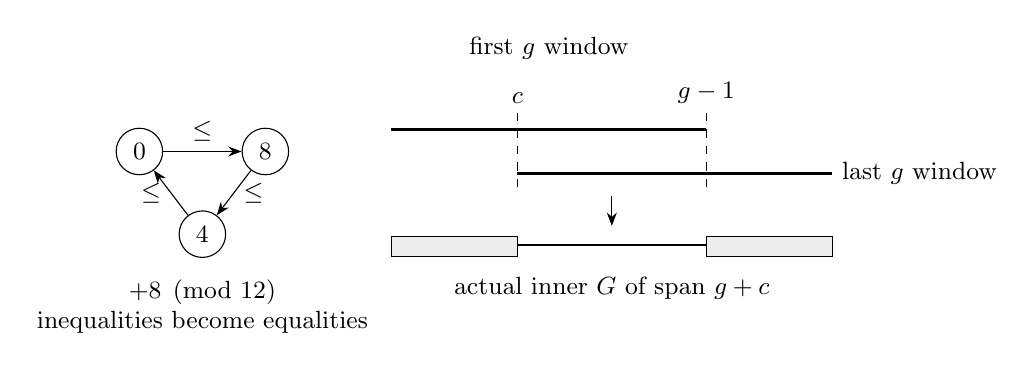
\begin{tikzpicture}[>=Stealth,font=\small,x=.8cm,y=.7cm]
 \node[circle,draw] (a) at (0,1.8) {\(0\)};
 \node[circle,draw] (b) at (2,1.8) {\(8\)};
 \node[circle,draw] (c) at (1,.3) {\(4\)};
 \draw[->] (a)--node[above] {\(\le\)}(b);
 \draw[->] (b)--node[right] {\(\le\)}(c);
 \draw[->] (c)--node[left] {\(\le\)}(a);
 \node[below,align=center] at (1,-.35) {\(+8\pmod {12}\)\\inequalities become equalities};
 \draw[thick] (4,2.2)--(9,2.2);
 \draw[thick] (6,1.4)--(11,1.4);
 \draw[dashed] (6,1.15)--(6,2.5);
 \draw[dashed] (9,1.15)--(9,2.5);
 \node[above] at (6,2.5) {\(c\)};\node[above] at (9,2.5) {\(g-1\)};
 \node[above] at (6.5,3.3) {first \(g\) window};
 \node[right] at (11,1.4) {last \(g\) window};
 \draw[->] (7.5,1)--(7.5,.45);
 \draw[fill=gray!15] (4,-.1) rectangle (6,.25);
 \draw[thick] (6,.1)--(9,.1);
 \draw[fill=gray!15] (9,-.1) rectangle (11,.25);
 \node[below] at (7.5,-.3) {actual inner \(G\) of span \(g+c\)};
\end{tikzpicture}
\caption{Left: one gcd cycle in the arithmetic illustration \(p=12,q=8\).
Right: the retained end windows agree on their singleton-aligned overlap
and form the actual folded inner.  Shaded end bands contain the explicitly
constructed width-\(c\) marks; their cells are selected in the proof.
Neither panel asserts an example of a contradictory original minimal pair.}
\label{fig:cycles-fold}
\end{figure}

Use a whole antitransposition, when necessary, to put the original chart
in case (a) or (d); it will be undone on the final construction.  Let
\(\rho=0\) for a row source outer and \(\rho=1\) for a column source outer.

\smallskip\noindent\emph{Ordinary source.}
The actual interior coding gives
\(A_S(jp+t)=B_S(jp+s)=\rho\).
Write \(\tau=t\bmod g\), \(\sigma=s\bmod g\); then
\begin{equation}\label{eq:fold-slots}
 A_\tau^0=B_\sigma^0=\rho.
\end{equation}
The only initial and terminal deviations from the generic words yield
\[
 \begin{array}{c|cc}
 \rho=0&t=\tau\in[0,c]&s=bg+\sigma,\quad\sigma\in[0,c]\\
 \rho=1&s=\sigma\in[1,c]&t=bg+\tau,\quad\tau\in[0,c-1].
 \end{array}
\]
These bounds follow by comparing each exceptional cap bit with its
existing period-\(p\) interior occurrence.  Every other cap step is generic.
If \(i=\one_{\tau>0}\), \(j=\one_{\sigma<c}\), the four pins give
\begin{equation}\label{eq:fold-cap-budget}
 C_0=i(1-\rho)+\rho,\quad
 -C_c=\rho+j(1-\rho),\quad
 \sum_{r=1}^{c-1}C_r+(i-j)(1-\rho)=0.
\end{equation}
The initial correction is \(i\) for \(\rho=0\) and one for \(\rho=1\);
zero drift and \(H_{g-1}=1\) identify it with \(C_0\), and \(H_c=1\) gives
the partial sum.  The terminal calculation gives the second relation.

Choose the new case (a) when \(\rho=1\), or when \(\rho=0\) and
\(\tau<\sigma\).  Choose the new case (b) otherwise.  In the latter case
\(\tau>0\) and \(\sigma<c\): the forbidden pair \((0,0)\) would leave the
original positive mark's diagonal at \(bg\) empty (or violate \(s\ge1\)
when \(b=0\)), and \((c,c)\) would leave the initial diagonal \(c-1\) empty
(or violate \(t<w\) when \(b=0\)).

The retained marked copies on \(G\) are defined cell by cell:
\[
 \begin{array}{c|cc}
 \text{new case}&\text{delete in lower band }r&
                         \text{delete in upper band }g+r\\\hline
 (a)&\text{southeast cell for }r\ge\sigma&
                         \text{northwest cell for }r<\tau\\
 (b)&\text{northwest cell for }r\ge\tau&
                         \text{southeast cell for }r<\sigma.
 \end{array}
\]
Retain every other cell.  In case (a), their common internal words are
the generic words with the internal \(A\)-slot \(\tau\) and \(B\)-slot \(\sigma\)
set to one; in case (b), those slots are set to zero.
\Cref{eq:fold-slots,eq:fold-cap-budget} give binary steps and singleton ends.

Their heights are positive.  For \(\rho=1\) the new lower mark has exactly
the first \(c\) diagonal heights of the original positive mark.  For
\(\rho=0\) the original mark has height
\begin{equation}\label{eq:old-mark-height}
 H_{r\bmod g}^0+\one_{t>0,\ r\ge t}-\one_{r\ge s}.
\end{equation}
When \(\tau<\sigma\), the new height is
\(H_r^0+\one_{\tau>0,r\ge\tau}-\one_{r\ge\sigma}\).
Before \(\sigma\) it is an initial-parent height; afterward it is
\eqref{eq:old-mark-height} at \(bg+r\).  In the new case (b) it is \(H_r^0\),
positive from the initial parent for \(r<\tau\) and from the old mark for
\(r\ge\sigma\).  These ranges cover every marked residue.  Thus the retained
copies are congruent connected skew diagrams, with a translation of
content \(g\).

For new case (a), the middle consists of a southeast singleton lower tail,
the private band, and a northwest singleton upper tail.  Their joins are
actual singleton diagonals; inherited endpoint steps give both connected
one-mark complements.  The actual bits \(B_\sigma=0\) and
\(A_{g+\tau}=0\) give the horizontal attachments.  Separation is \(c<g\).
Write the displacement as \((h,h+g)\).  Any containing mark on the same
\(c\) content diagonals sends the southwest singleton into content \(g\),
forcing \(h'\le h\).  At relative content \(\tau<c\) the upper tail has
ended; the northwest retained cell forces \(h'\ge h\).  At this displacement
the mark is exactly \(G\cap(G-(h,h+g))\), proving maximality against every
possible displacement.  The hatted middle is confined to \([c+1,g-2]\);
all periodic hatted-mark cells have residues \(0,\ldots,c-1\).  Their content
distance is at least two, proving the entire bi-infinite condition IV.
Whole antitransposition gives the corresponding checks for new case (b).

Define the new outer bits by
\[
 (A_j^{D_L},B_j^{D_L})=
 \begin{cases}
 (A_S(jg+\tau),B_S(jg+\sigma)),&(a),\\
 (1-B_S(jg+\sigma),1-A_S(jg+\tau)),&(b).
 \end{cases}
\]
They form a constant equal pair by \eqref{eq:fold-slots}, hence an actual
row or column of \(L\) cells.  The complete coding reconstructs every source
step and both defining windows of \(G\), so its composition is literally \(S\).

\smallskip\noindent\emph{Mixed source.}
Normalize to case (d).  Its fixed word gives \(B_0^0=0\), \(B_c^0=1\) and
its original slots give \(A_S(jp+t)=\rho\), \(A_S(jp+s)=1-\rho\).
The two projected slots are distinct, because otherwise one generic bit
would have to equal zero and one.  Let \(z_0\) be the original phase with
generic bit zero and \(o_0\) the phase with generic bit one.  Synchronization
confines the initial correction and terminal deficit to
\(0\le z_0\le c\) and \(bg\le o_0\le bg+c\).  Put
\[
 \tau=z_0,\quad\sigma=o_0-bg,\quad
 \alpha=\min(\tau,\sigma),\quad\beta=\max(\tau,\sigma).
\]
Then \(0\le\alpha<\beta\le c\) and
\[
 C_0=\one_{\tau>0},\qquad -C_c=\one_{\sigma<c},\qquad
 \sum_{r=1}^c C_r=-C_0.
\]
A wide mixed column source is automatically excluded by \(t<s\) and these
bounds, but the narrow column source remains in the construction.

The same window union \(G\) has southeast displacement
\(\lambda=(-h,g-h)\), where \(h=\sum_{r=0}^{g-1}B_r^0\).
Delete the northwest cell from lower marked residues \(r\ge\beta\) and
upper marked residues \(g+r\) with \(r<\alpha\).  Before deletion their heights
are
\[
 L_r=H_r^0+\one_{\tau>0,r\ge\tau},\qquad
 U_r=H_r^0+\one_{\tau>0}-\one_{\sigma<c,r\ge\sigma}.
\]
After deletion both are
\[
 \begin{cases}
 H_r^0+\one_{\tau>0,r\ge\tau}-\one_{r\ge\sigma},&\tau<\sigma,\\
 H_r^0,&\tau>\sigma.
 \end{cases}
\]
Positivity follows from the initial parent before \(\sigma\) and the original
mark at \(bg+r\) afterward in the first case.  In the second, if \(b=0\) it
is the old mark; otherwise the initial range \(r<\tau\) and old-mark range
\(r\ge\sigma\) cover every residue.  Their southeast word is \(B^0\) and
their northwest word is \(A^0\) with internal slots \(\alpha,\beta\) set to
one and zero.  The budget gives singleton ends, so the retained copies are
congruent, connected and southeast-justified, with the stated displacement.

The middle has two northwest singleton tails and the private band.  Its
inherited steps and singleton joins prove both complements connected.  The
bits \(A_\beta=1\) and \(A_{g+\alpha}=0\) give the vertical/horizontal
attachments, including \(\alpha=0\) through the actual private endpoint.
For maximality, the image of the southwest singleton gives
\(\lambda'_1\le\lambda_1\); the inverse image of the northeast singleton
in the lower content-\(c-1\) interval gives the reverse inequality.  At that
displacement the deleted-tail ranges are disjoint, so the mark is the full
intersection.  The same content-distance argument proves IV, including
neighbors outside the retained mark.  Finally define
\[
 A_j^{D_L}=A_S(jg+\alpha),\qquad
 B_j^{D_L}=1-A_S(jg+\beta).
\]
The generic slot bits sum to one, so these are a constant equal pair.
The full mixed coding, with every supplemental copy, reproduces the two
original words and both windows.  This proves \eqref{eq:actual-fold};
whole antitransposition gives case (c).

The formulas include \(c=1\) directly.  Since \(g\ge2\), \(G\) is proper, and
\(L\ge4\) makes the outer proper.  Undo all full transports on the constructed
chart.  No minimum on \(G\) or on a coface has been used.
\end{proof}


\subsection{Completion of period rigidity}

\begin{proof}[Proof of \Cref{thm:main}]
Suppose \(p>q\).  \Cref{thm:reduction} excludes every original input except
\eqref{eq:hard-domain}.  In that case \Cref{prop:whole-structure,lem:phase-confinement}
provide the whole-parent structure, actual caps and original \(p\)-period.
\Cref{prop:clocks} excludes opposite types and aligns the ordinary clocks.
\Cref{thm:end-filter,thm:scalar-synchronization} give all private \(q\)-shift
equalities or a single consistent direction of inclusion.  The budget
\eqref{eq:cycle-budget} and \Cref{lem:cycles} give both full original
\(g\)-periodic boundary words, with the original singleton pins retained.

\Cref{thm:fold} now constructs the actual same-source chart before its
score is compared with the prescribed original score:
\[
 (c,g+c)<(bg+c,(A+b)g+c).
\]
If \(b>0\) the width improves; if \(b=0\) the inner span improves because
\(g<p\).  This contradicts the source's own minimum.  Hence \(p=q\).
Every lower-class call occurred at a stated strict area, except for the
same-area zero-free class theorem proved independently from strict erosion.
\end{proof}

\begin{corollary}\label{cor:equal-width-ribbon}
Let \(F=D\circ_\omega E\) and \(H=C\circ_\eta U\) be actual proper legal
I--IV charts with \(s_F=s_H\) and common period \(p\).  If \(D\) is a
ribbon, their overlap widths agree, \(N_D=N_C\), and \(C\) is a ribbon.
\end{corollary}
\begin{proof}
Write \(w,u\) for the overlap widths and \(N\) for the common span.
The span law gives \(N=pN_D+w=pN_C+u\).
Since \(0\le w,u<p\), it follows that \(w=u\) and \(N_D=N_C\).
The complete proper corners agree.  By \eqref{eq:exact-corner-transport},
the ribbon-source corner contains only factors of span less than \(p\).
A positive component \(T\) of \(C^-\) would contribute the connected prime
\(s_{T\circ_\eta U}\) of span \(pN_T+u\ge p\) to the equal complete corner,
which is impossible.  Thus \(C^-=\varnothing\).
\end{proof}

\section*{Concluding remarks}
The period comparison separates algebraic synchronization from geometric
reconstruction.  Core reduction and diagonal heights recover the expected
gcd structure but leave paired boundary choices undetermined.  Extreme
component residues exclude the choices that could defeat noncancellation;
the entire differential identity then forces the remaining comparisons.
For mixed charts a directed inclusion suffices, because finite period
cycles turn it into equality.  The synchronized words construct the legal
finer chart on the original source, and that chart makes source minimality
decisive.

This proves the ribbon-outer period step under the strict lower-area joint
package.  Equal-period marked-factor and prescribed-fiber identification is
a different assertion.  Root existence and the positive-interior induction
steps are also separate.  The method here is the
passage from complete determinant identities to literal boundary
constraints without an exhaustive classification of their intermediate
rational response representations.


\appendix
\section{Aligned reconstruction before minimality}\label{app:aligned}

This appendix proves the reconstruction assertion used in
\Cref{prop:aligned-reconstruction}.  The two original parents, the source
ribbon, the prescribed fine minimum and \(\Jlower\) remain fixed.  The displayed
coarse chart is not required to be minimal.  Write
\[
 p=kq,\qquad w=bq+u,\qquad 0\le b<k,\quad0\le u<q,
 \qquad R=k+b,\quad N_E=Rq+u.
\]
The letter \(P\) below denotes a reduced coarse polynomial, not an assumed
skew Schur function.

\subsection{The actual composition operators}

For a fixed marked inner of period \(d\), let \(A,B,C\) be its mark, hatted-mark
and hatted-middle functions.  All these factors use generators below \(d\).
Use the row-generator map of \eqref{eq:phi}, with the ordinary involution
carried whenever the chart is changed.  Its fresh coefficient at \(h_{jd+v}\),
where \(v\) is the width, is nonzero, primitive, and uses only generators below
\(d\).  This follows by expanding the actual row-probe determinant at its
unique largest entry and applying the full corner transport formula.

Use composition covariance and terminal readout from
\cite{Shields2026Readout}, with the actual row map \eqref{eq:phi}
and full normalizer \eqref{eq:normalizer}.  In the ordinary case (a),
write \(\xi=\delta_d s_E\) and \(\theta=V_d s_E/\xi=s-t\).
For case (b) the read map is \(\Phi_\omega\circ\iota\) and the read outer
is \(\iota(s_D)\); the actual \(\xi=\delta_d s_E\) and
\(\theta=V_d s_E/\xi\) carry the physical signs.  In either ordinary
reading \(|\theta|<d\), and
\[
 \delta_{rd}\Phi=\xi^r\Phi\delta_r,\qquad
 V_{rd}\Phi=\xi^r\Phi(dV_r+\theta\delta_r).
\]
The genuine empty edges have \(\theta=0\).
For a mixed chart rotate the whole chart to case (d), put
\(\rho=s-t\in(0,d)\) and \(\chi=(-1)^{-v_1}ABC\), and use
\[
 \delta_{rd}\Phi=0,\qquad
 V_{rd}\Phi=\chi^r\Phi(dV_r+\rho\delta_r).
\]
Here \(\Phi(1)=1\) is the algebraic unit.  An exhausted row probe
instead has geometric remainder \(b_0=A\); the cited identities retain
that local factor.  Whole antitransposition obeys
\(\delta_j\iota=(-1)^{j-1}\iota\delta_j\) and
\(V_j\iota=(-1)^j\iota V_j\), and transports the map, outer involution,
and entire normalizer together.

For the terminal application take the original ribbon source
\(F=D\circ_\omega E\) of period \(p\), with \(M=|D|\ge2\).
Terminal readout \cite[Terminal readout]{Shields2026Readout} gives
\[
 \begin{aligned}
 \frac{\delta_p^{M-1}s_F}{\delta_p^M s_F}
   &=\frac{s_E}{\xi_s}&&\text{in the ordinary case},\\
 \frac{V_p^{M-1}s_F}{V_p^M s_F}
   &=\frac{s_E}{\rho_s\chi_s}&&\text{in the positive-phase mixed case}.
 \end{aligned}
\]
Here \(\xi_s=\delta_p s_E\) in the ordinary source; in the rotated
mixed source, \(\rho_s=s_s-t_s\) and
\(\chi_s=(-1)^{-(v_s)_1}A_sB_sC_s\) use that source's own phases,
displacement, and three local factors.
Both denominators are nonzero, and the full source normalizers cancel.
The elementary-generator identities used for the line observers are
\[
 \begin{aligned}
 (dV_r+\rho\delta_r)h_j&=(d(j-r)+\rho)h_{j-r},\\
 (dV_r+\rho\delta_r)e_j&=(-1)^{r-1}(\rho-d(j-r))e_{j-r}
 \end{aligned}
 \qquad(j\ge r).
\]
For \(j<r\) both outputs vanish.  At exhaustion the scalar output is
not assigned to a proper one-cell or empty chart.

\begin{proposition}\label{prop:full-image}
Let \(F=D\circ_\omega E\) and \(H=C\circ_\eta U\) be actual proper legal
I--IV charts with equal whole Schur functions, of periods \(p,q\) and
overlap widths \(w,u\), respectively.  Suppose \(D\) is a ribbon with
\(M=|D|=N_D\ge2\), and
\[
 p=kq,\qquad k\ge2,\qquad w=bq+u,\qquad
 0\le b<k,\quad 0\le u<q.
\]
Put \(R=k+b\), so \(N_E=Rq+u\).  Use the complete fine map
\(\Phi_\eta\) of \eqref{eq:phi}, carrying the outer involution and the
full local normalizer whenever a physical frame is changed.
Then either the two original operator types are incompatible, or one
obtains a primitive irreducible weighted-homogeneous polynomial
\(P\in\Z[h_1,h_2,\ldots]\), linear in its largest generator \(h_R\), and
a nonzero primitive low polynomial \(L\) such that
\begin{equation}\label{eq:full-source-image}
 \Phi_\eta(P)=L s_E.
\end{equation}
Here \(\spn(P)=R\), and \(L\) uses only the original generators below \(q\).
This construction does not assume a chart on \(E\) through \(U\).
Neither source-minimality nor a lower-area classification hypothesis is
required for this extraction.
\end{proposition}
\begin{proof}
Apply composition covariance to the two original source words in terminal
readout \cite[Composition covariance and terminal readout]{Shields2026Readout}.
If an ordinary source is paired with a mixed
fine chart, its nonzero terminal Hall word is incompatible with the fine
Hall zero.  Otherwise let \(T_1,T_0\) be the two complete coarse outputs.  The
fine normalizer cancels in their ratio, giving
\begin{equation}\label{eq:ratio-readout}
 \Phi_\eta(T_1/T_0)=R_{<q}\,s_E/X_s,
\end{equation}
where \(X_s=\xi_s\) or \(\rho_s\chi_s\), and \(R_{<q}\) is a nonzero fine low
factor.  Every connected factor of \(X_s\) has span below \(p\), but \(X_s\) is
not assumed to have span below \(q\).  Since \(N_E=p+w\ge p\), it is coprime to
the actual connected polynomial \(s_E\).

Reduce \(T_1/T_0=P/G\) before interpreting the numerator, with \(P,G\) coprime
and weighted homogeneous, and make \(P\) primitive integral.  Put
\(x_j=h_{jq+u}\).  At a finite cutoff write the actual fine generators as
\(\Phi_\eta(h_j)=c_jx_j+d_j\),
where \(c_j\) is a nonzero primitive low polynomial and \(d_j\) uses earlier
raw labels.  Adjoin the fraction field \(K\) of all nonpivot raw variables.
Triangular substitution is an isomorphism over \(K\), so \(\Phi(P)\) and
\(\Phi(G)\) are coprime there.  Equation \eqref{eq:ratio-readout} and the
connected prime \(s_E\), which depends on the fresh pivot \(x_R\), give
\(\Phi(P)=c_Ks_E\) for \(c_K\in K^\times\).

Write \(c_K=a/b\) in coprime nonpivot polynomials.  Polynomiality would make
\(b\) divide \(s_E\).  Since \(s_E\) is irreducible and depends on \(x_R\), \(b\) is
constant.  Thus \(c_K\) is a nonpivot polynomial.  Order the selected pivots
from largest to smallest.  The leading selected-monomial coefficient of
\(\Phi(P)\) is a nonzero rational coefficient of \(P\) times a product of the
\(c_j\), hence is low.  Every purely nonpivot factor consequently divides a
low polynomial and is low up to a rational unit.  This proves
\eqref{eq:full-source-image}.

The same primitive pivot argument modulo each integer prime shows that
\(\Phi(P)\) is primitive.  Gauss's lemma makes \(L\) primitive after absorbing
the original rational scalar.  The unique largest pivot of \(s_E\) then
shows that \(P\) has span \(R\) and is linear in \(h_R\).  Any factorization of
\(P\) would, under the triangular isomorphism, factor the one connected
high prime; a nonconstant coarse factor cannot become a coefficient-field
unit.  Hence \(P\) is irreducible.  Only the original words of lengths \(M-1\)
and \(M\) were used.
\end{proof}

\begin{lemma}\label{lem:derivative-stock}
The polynomial \(\partial_{h_R}P\) is, with its canonical sign, a primitive
positive product \(\Gamma\) of connected component functions from the actual
fine outer interior.  Multiplicities are retained.  A cell component
contributes \(h_1\); a noncell component provides a proper fine reference.
\end{lemma}
\begin{proof}
Differentiate \eqref{eq:full-source-image} at its unique largest pivot:
\[
 c_R\Phi_\eta(\partial_{h_R}P)=L\,\partial_{h_{N_E}}s_E.
\]
The complete source proper corner divides the proper corner of \(F\):
for a ribbon outer the latter is
\(\Theta_s A_s^{r(D)-1}B_s^{c(D)-1}C_s^M\), whereas
\(\kappa(E)=\Theta_s C_s\).  Every high connected factor of that same corner,
read on \(H\), is the function of an actual component \(Z\) of \(C^-\) composed
through the original \(\eta/U\); every other fine factor is below \(q\).
Triangular prime transport and coefficient-field independence identify
all coarse factors of \(\partial_{h_R}P\) with these actual \(s_Z\), including
their exponents.  Primitive pivot coefficients retain integer content.
The actual positive proper coefficient fixes the canonical sign.
A noncell \(Z\) has at least two cells and makes \(Z\circ_\eta U\) proper;
a cell makes only the function \(s_U\) and is not assigned such a chart.
\end{proof}

\subsection{Distinct phases retain the entire coarse polynomial}

\begin{lemma}\label{lem:distinct-leading}
Let the fine positive mark have distinct phases.  Its actual marked core
map has a fixed \(\gamma\in\{\mathrm{id},\AT\}\) and a legal mark \(\eta_0\)
on \(U_0=\Core(U)\).  For every nonzero weighted-homogeneous coarse polynomial
\(f\) of weight \(d\),
\begin{equation}\label{eq:distinct-leading}
 \operatorname{in}_{\rm ord}\Phi_\eta(f)
   =\epsilon^d\Phi_{\eta_0}(\iota_\gamma f),\qquad
 \ord_{\rm ord}\Phi_\eta(f)=d\,r(U_0),
\end{equation}
where \(\epsilon\) is the actual core phase and \(\iota_\gamma\) is the
identity or the carried involution.  In particular the input on the right
is the whole \(f\), not its initial ordinary-degree part.
\end{lemma}
\begin{proof}
At distinct phases the transformed mark itself is zero-free: each tail
operation either removes one boundary bit or adds a bit where the other
bit is zero.  Thus its function \(A_0\) is ordinary homogeneous.  The actual
row-probe core has \(r(\Row_j\circ U_0)=j r(U_0)-(j-1)r(W_0)\),
so \(\Phi_{\eta_0}(h_j)\) is homogeneous of ordinary degree \(j r(U_0)\).
The elementary-probe normalization gives the analogous assertion for its
other mark factor \(B_0\).

Put \(\Psi=\Phi_{\eta_0}\), and let \(A^*,B^*\) be the positive ordinary
cores of the original mark and hatted-mark products.  Their actual
initial signs are included in the phases below.
The geometric core formula gives
\[
 G_j:=\operatorname{in}_{\rm ord}\Phi_\eta(h_j)
   =\epsilon_j\vartheta^{j-1}\Psi(\iota_\gamma h_j),
 \qquad G_1=\epsilon_1\Psi(h_1).
\]
The two actual two-cell probes give the following two normalizations:
\[
 \begin{array}{c|cc}
 \gamma&G_2&
 H_2:=\operatorname{in}_{\rm ord}\Phi_\eta(e_2)\\ \hline
 \mathrm{id}&\epsilon_2(A^*/A_0)\Psi(h_2)&
             \epsilon'_2(B^*/B_0)\Psi(e_2)\\
 \AT&\epsilon_2(A^*/B_0)\Psi(e_2)&
       \epsilon'_2(B^*/A_0)\Psi(h_2).
 \end{array}
\]
Call the first ratio \(\vartheta\) and the second \(\vartheta'\).
They are positive primitive low Schur-product ratios.
If \(d_A,d_B\) are their ordinary degrees, the competing degrees in
\(\Phi_\eta(e_2)=\Phi_\eta(h_1)^2-\Phi_\eta(h_2)\) are
\[
 \deg_{\rm ord}G_1^2=2r(U_0),\qquad
 \deg_{\rm ord}G_2=2r(U_0)+d_A,\qquad
 \deg_{\rm ord}H_2=2r(U_0)+d_B.
\]
If \(d_A>0\), the initial difference is the square of \(s_{U_0}\),
whereas the actual column probe has one connected two-copy prime.
Their low normalization factors cannot reconcile these high primes.
If \(d_A<0\), the initial difference is \(-G_2\), identifying the row
and column two-copy primes up to a low factor, contrary to
\Cref{lem:faithful}.  Hence \(d_A=0\).

Put \(Y_j=\Psi(\iota_\gamma h_j)\).  In the independent fine pivot
coordinates, \(Y_1^2,Y_2\) are distinct monomials, so their difference
cannot lose its degree.  Both terms survive, and
\[
 Y_1^2-\epsilon_2\vartheta Y_2
   =\epsilon'_2\vartheta'(Y_1^2-Y_2).
\]
Comparison of the two coefficients gives
\[
 \epsilon'_2\vartheta'=1,\qquad \epsilon_2\vartheta=1.
\]
Positivity gives \(\vartheta=\vartheta'=1\) and
\(\epsilon_2=\epsilon'_2=1\).
For \(j\ge3\), use the actual hook \((j-1,1)\), whose function is
\(h_1h_{j-1}-h_j\).  Its normalization is \(A^{j-2}B\).
The two calibrated ratios make its core normalization agree with
that of the carried hook, also when the roles of \(A_0,B_0\) are
exchanged.  For its actual core phase \(\eta_j\), the initial identity is
\[
 \epsilon_1\epsilon_{j-1}Y_1Y_{j-1}-\epsilon_jY_j
   =\eta_j(Y_1Y_{j-1}-Y_j).
\]
Comparing the two independent coefficients gives
\(\epsilon_j=\eta_j=\epsilon_1\epsilon_{j-1}\).
Together with \(\epsilon_2=\epsilon_1^2=1\), this yields
\(\epsilon_j=\epsilon_1^j\).
Triangular independence prevents cancellation
for any nonzero weighted-homogeneous input and proves
\eqref{eq:distinct-leading}.  These are identities of known fine probe
compositions, not new observations on the source.
\end{proof}

\begin{proposition}\label{prop:distinct-realization}
If the original fine mark is positive and distinct, the polynomial \(P\) of
\Cref{prop:full-image} is the canonically phased function of an actual
connected diagram of span \(R\).
\end{proposition}
\begin{proof}
Apply the actual marked-core construction to the original equal parents.
The zero-free class theorem and \Cref{prop:class-quotient} supply an actual
\(J_0\) of span \(R\) with
\(s_{E_0}=s_{J_0\circ_{\eta_0}U_0}\).  Apply
\eqref{eq:distinct-leading} to the entire image
\eqref{eq:full-source-image}.  Its initial right side is the actual core
function times a low factor.  The class-valued quotient gives that same
function as the normalized image of \(s_{J_0}\).  Therefore the images of
\(\iota_\gamma P\) and \(s_{J_0}\) differ by a low rational scalar.
In the independent fine pivot coordinates this scalar is rational
constant.  Primitivity and the actual top proper phase make it the
canonical sign.  Apply the physical identity or antitransposition to
\(J_0\) prescribed by \(\gamma\).  The resulting actual diagram realizes the
entire \(P\).
\end{proof}

\subsection{Whole coframes recover actual end windows}

The zero-offset reconstruction uses the weak-cap and absolute-flag
theorem of \cite{Shields2026Coframes}.  Its domain is arbitrary strictly
ordered positive lists \(X,Y\) with \(X_i\ge Y_i\), including unit and
disconnected proper blocks.  Its joint-polynomial numerator
irreducibility and reconstruction of the absolute flags from the whole
rational coframe are both retained; connected-coframe coprimality alone
would not supply this interface.  The application below is needed when
the fine outer interior contains a noncell, even if that factor comes
from a wide source mark rather than from \(E^-\).

A permitted transport here is the original marked \(U\), or its
simultaneous half-turn with both full end marks and their attachments,
up to translation.  Write \((U^\dagger,\eta^\dagger)\) for the chosen
representative.  An ordinary gauge is accompanied by its outer
involution and is undone before the row maps are compared; in the
original ordinary reading,
\(\Phi_{\eta^\dagger}=\Phi_\eta\).
The first and last \(q\) windows use this same representative, with
the lower window southwest-normalized and the upper window read in
its reflected end frame.  The transport is supplied by the original
minimum's smaller-area fiber, not by a new factorization of \(U\).

\begin{lemma}\label{lem:conormal-caps}
In the original aligned comparison, suppose the actual \(C^-\) has a
noncell component.  If the fine mark has zero offset, the first and last
\(q\) windows of the original \(E\) are the complete windows of one permitted
transport of the original marked \(U\).  Every cap unit is retained.
\end{lemma}
\begin{proof}
Choose a noncell \(Z\subset C^-\).  Its actual reference
\(Z\circ_\eta U\) is proper, and its connected function occurs as a high
factor of the common whole proper corner.  Each corresponding actual
component of \(F^-\) has area below \(n\).  By the original fine minimum,
\Cref{lem:oim,lem:lower-full} give it that same fine marked factor.
We use the \emph{whole parent} \(F\) for this argument, so the component may
come from a source mark or a hatted source piece, not only from \(E^-\).

At a finite cutoff put
\(y_j=\Phi_\eta(h_j)=c_jh_{jq+u}+d_j\), and retain all nonpivot raw variables
as spectators.  Over the fraction field of the raw variables below \(q\),
triangular inversion is polynomial in \(y_j\) and the high spectators.
Put \(K=N_C\), so \(N_F=Kq+u\), and use the current carried fine
frame.  If \(A_\eta,B_\eta,C_\eta\) are its local mark products, the
complete low normalization is
\[
 \mathcal N_\eta=\epsilon_\eta(C)
 A_\eta^{|C|-r(C)}B_\eta^{|C|-c(C)}C_\eta^{|C|-K}.
\]
The original whole equality and its top derivative give
\[
 \Phi_\eta(s_C)=\mathcal N_\eta s_F,\qquad
 c_K\Phi_\eta(\partial_{h_K}s_C)
    =\mathcal N_\eta\partial_{h_{N_F}}s_F.
\]
Any prescribed outer involution acts on both displayed coarse
polynomials.  The nonzero factor \(\mathcal N_\eta\) uses only raw
labels below \(q\); negative normalization exponents are read in that
low fraction field.
Define the partial compensator
\[
 \Delta_s^{<j}=\partial_{h_s}
       +\sum_{i<j}a_{si}\partial_{h_{iq+u}}.
\]
Differentiation in one spectator, holding all \(y_j\) fixed, is
\[
 \Delta_s=\partial_{h_s}+\sum_j a_{sj}\partial_{h_{jq+u}},\qquad
 a_{sj}=-c_j^{-1}\bigl((\Delta_s^{<j}c_j)h_{jq+u}
                              +\Delta_s^{<j}d_j\bigr).
\]
For a high spectator \(s\ge q\), induction on \(j\) gives \(a_{sj}=0\)
whenever \(jq+u<s\): the entire \(j\)th pivot polynomial uses only raw
labels at most \(jq+u\), and all earlier compensators are already zero.
Since \(s\) is not a selected pivot, the first possibly moving pivot is
strictly above \(s\).  Every raw label below \(s\) is fixed.  The low
coefficients \(c_j\) are fixed as well, but the lower terms \(d_j\) retain
their full earlier-pivot feedback in the displayed recursion.
These two identities express \(s_F\) and its complete proper product
as polynomials in the \(y_j\) over the low fraction field, independent
of the high spectators.  Degree additivity in each spectator makes
every connected factor of the proper product independent of it as well.

Fix one high component prime and retain every one of its \(e\) actual
occurrences \(G_1,\ldots,G_e\), in their original order.  Eliminate all regular
components and unit records by their full block inverses.  The resulting
proper matrix is upper block triangular, with the unchanged diagonal
blocks \(G_i\) and complete effective bridges \(E_{i,i+1}\).  Modulo the selected
prime, each \(G_i\) has rank one less than its size.  Its proper corner is a
nonzero coefficient-field unit: differentiate its actual fine image at
\(h_{vq+u}\), obtaining a nonzero multiple of
\(\Phi(\partial_{h_v}s_Z)\), which is not divisible by the prime.
Normalize the rank-one adjugates using these corners.  Their vectors remain
polynomial in the spectators.

The only maximal-pole path visits all \(e\) occurrences.  The complete source
residue is a nonzero coefficient-field scalar times
\begin{equation}\label{eq:ordered-conormal-chain}
 (u_{\mathrm{eff}}a_1)
 \prod_{i=1}^{e-1}(b_i^tE_{i,i+1}a_{i+1})
 (b_e^tg_{\mathrm{eff}}).
\end{equation}
The final factor contains the actual creation column.  The source is a
connected prime of larger span, so its residue is nonzero.  Polynomial
degree additivity in each spectator therefore makes every complete link
in \eqref{eq:ordered-conormal-chain} spectator-flat.

Each link has an actual connected numerator.  For consecutive occurrences,
retain all intervening regular records, delete the last column of \(G_i\)
and the first row of \(G_{i+1}\), and nothing else.  Between these deletions an
old row pairs with the next old column; positive rows and the old weak
diagonals prove connectedness, including all intervening unit records.
If there are \(\ell\) regular records, its raw determinant is
\[
 (-1)^\ell\det(H_{\mathrm{reg}})
 e_{\mathrm{last}}^t\adj(G_i)E_{i,i+1}\adj(G_{i+1})e_{\mathrm{first}}.
\]
The sign follows by moving \(\ell\) regular rows past \(r(G_i)\) rows and the
matching columns past \(r(G_i)-1\) columns.  At the left end keep the original
first row and delete the first row of the first component; at the right
end delete the last component column and keep the original column \(0\).
The endpoint signs are the same total-regular-rank signs.  Their proper
corners are products of regular determinants and nonzero component
corners, hence nonzero in the residue field.

If such a numerator had high nonpivot span \(d\), then \(\Delta_d\) would act
on it simply as \(\partial_{h_d}\), since every compensating pivot is higher
than \(d\).  Its derivative is its nonzero proper corner, contradicting
spectator-flatness.  Thus every endpoint and consecutive span is \(jq+u\).
The left endpoint gives \(\min Y(G_1)\equiv0\pmod q\); consecutive spans
propagate this congruence, and every component maximum is congruent to
\(u\).  The right endpoint gives the same final phase.  Repeat the argument for
every high prime in the complete proper product, including the image of
a one-cell component.  Thus all high component occurrences have aligned
absolute endpoints before any last-band bound is used.

The last-band bound follows from these actual aligned occurrences.
Every high connected factor of the proper corner of \(F\), of span
\(N_F=Kq+u\), has smaller aligned span \(vq+u\); hence \(v\le K-1\).
All remaining factors have span below \(q\).
For an actual endpoint or consecutive numerator of span \(jq+u\), its
complete proper coefficient is the product of the intervening regular
component determinants and one or two repeated-component proper corners.
A regular high component lies strictly inside the numerator endpoints.
Its aligned endpoints give span \(vq+u<jq+u\), hence at most
\((j-1)q+u\).  For a repeated component of span \(vq+u\), the full fine
corner formula bounds its high proper factors by \((v-1)q+u\);
its local factors have span below \(q\).  This also covers a one-cell
occurrence, whose proper factors are all low.  The proper coefficient
of \(F\) is fixed on \((K-1)q+u<s<Kq+u\); that of each actual link
numerator is fixed on its corresponding band \((j-1)q+u<s<jq+u\).

Write \(X_F=(N_F,I_F)\) and \(Y_F=(C_F,0)\) for the whole parent's
full beta lists.
Let \(g_F=R_F\) be the complete lower endpoint coframe and
\(g_{F^*}=L_F\) the reflected upper endpoint coframe in the actual beta
frame of \(F\), as in \eqref{eq:gradient-product}.  Their normalizations
are at the actual bottom column and top row.  Let \(g_{U,-},g_{U,+}\)
be the corresponding whole weak-cap coframes obtained by solving the
known first and last \(q\)-window matrices of the supplied marked \(U\),
including all their unit records.  These native window coframes have
degree less than \(q\).  At this point the source coframes are only read
modulo \(z^q\); their full matrices have not been truncated, and physical
boundedness of the source caps has not been assumed.

Differentiate the whole-parent image above at a raw label in its
last open \(q\)-band.  Earlier selected images use smaller labels,
and later pivots exceed \(N_F\), so only \(y_K\) contributes.
Divide the summed derivative by the nonzero top cofactor, which
is fixed on this band.  The intrinsic full gradient and the actual
\(K\)th native row-probe give,
for \(0\le t<q\),
\[
 [z^t]g_Fg_{F^*}
 =\frac{\partial_{h_{N_F-t}}s_F}{\partial_{h_{N_F}}s_F}
 =\frac{\partial_{h_{Kq+u-t}}y_K}{c_K}
 =[z^t]g_{U,-}g_{U,+}.
\]
The case \(t=0\) is the common normalization one.  Thus
\begin{equation}\label{eq:whole-cap-product}
 g_F(z)g_{F^*}(z)=g_{U,-}(z)g_{U,+}(z)\pmod {z^q}
\end{equation}
Decompose each endpoint proper system at its actual zero-height cuts
and unit pivots, retaining every triangular bridge.
Suppose a block meeting a column of exponent below \(q\) has a
largest outer label \(d\ge q\).  Choose \(d\) maximal across both
endpoint systems, and then the earliest column exponent \(b\) at
which it occurs.  Since the constant coframe term is one,
\(0<b<q\).

Each block attaining \((d,b)\) is connected, of span \(s=d-b>0\).
Its matrix and all lower blocks omit \(h_d\); that variable occurs
only in the first entry of its effective creation border, with
coefficient one.  The inverse corner therefore gives
\[
 \partial_{h_d}[z^b](g_Fg_{F^*})
   =-\sum_{T\in\mathcal E_{d,b}}\frac{\kappa(T)}{Q_T},
\]
where \(\mathcal E_{d,b}\) consists of the one or two endpoint blocks
attaining the same earliest border.  Earlier colors are independent
of \(h_d\), so no product of two moving terms contributes.
This is ordinary differentiation of the selected rational
coefficient, not extraction of an \(h_d\)-coefficient or a residue.
For every such block,
\[
 \frac{Q_T}{\kappa(T)}=h_s-\omega_T,\qquad
 \omega_T\in\Q(h_1,\ldots,h_{s-1}).
\]
Regard the sum as a rational function of \(h_s\) over
\(\Q(h_i:1\le i<d,\ i\ne s)\).
Distinct monic factors have separate residues \(-1\); coincident
factors contribute their negative multiplicity.  The sum is
nonzero.  But the right side of \eqref{eq:whole-cap-product} uses
only raw labels below \(q\), so its \(h_d\)-derivative is zero.
This contradiction proves that both endpoint systems are physically
bounded below \(q\).

Their completed low blocks have equal row and column counts:
\[
 \#(I_F\cap[1,q))=\#(C_F\cap[1,q)).
\]
Thus \eqref{eq:height-beta} gives \(H_F(q-1)=1\).
The reflected upper count gives \(H_F(N_F-q)=1\).
These are singleton cuts in the full source lists, including every
common beta.

Apply the same last-\(q\) gradient to each actual link numerator above.
The proved bound on its complete proper coefficient makes that
coefficient fixed on the entire last open band.  Its conormal equation
has only the raw derivative there and the last-pivot compensation;
all lower compensators vanish and all higher pivots exceed its span.
Division by its actual nonzero proper coefficient gives
\eqref{eq:whole-cap-product} modulo the selected high prime, with all
occurrences and their original normalization retained.  After taking
the physically bounded caps, every coefficient belongs to the raw low
field.  The high prime has an independent fresh pivot, so reduction
modulo that prime is injective on this field.  The identity is therefore
an exact truncated low identity.
For each selected noncell occurrence \(G_i\), let \(V_i\) be the
permitted transport of the original marked \(U\) supplied by its
strict-area full fiber.  Its first and last \(q\)-windows survive
deletion of the opposite extreme flag, since \(N_{G_i}\ge2q+u\).
Write \(g_{F,-},g_{F,+}\) for the bounded lower and reflected upper
source caps.  All these coframes have constant term one and degree
below \(q\).

The left endpoint numerator retains the upper source window and
the lower window of \(G_1\).  Its normalized last-band identity is
\[
 g_{F,+}g_{V_1,-}
   \equiv g_{U,+}g_{U,-}
   =g_{V_1,+}g_{V_1,-}\pmod{z^q}.
\]
The last equality carries the permitted rotation or ordinary gauge:
rotation exchanges the two endpoint coframes, while the ordinary
gauge leaves the inner diagram unchanged.
Cancellation takes place in
\(\Q(h_1,\ldots,h_{q-1})[z]/(z^q)\), where \(g_{V_1,-}\) is a unit,
and gives
\[
 g_{F,+}\equiv g_{V_1,+}\pmod{z^q}.
\]
Both polynomials have degree below \(q\), so they are equal as whole
coframes.  Their actual weak cap lists are strictly ordered and positive,
with \(X_i\ge Y_i\); no unit or disconnected block has been removed.
The weak-cap and absolute-flag theorem
\cite{Shields2026Coframes} therefore identifies their complete absolute flags.

The numerator between \(G_i\) and \(G_{i+1}\) retains the upper
window of \(G_i\) and the lower window of \(G_{i+1}\).  Its complete
normalized identity is
\[
 g_{V_i,+}g_{V_{i+1},-}
   \equiv g_{U,+}g_{U,-}
   =g_{V_i,+}g_{V_i,-}\pmod{z^q}.
\]
Cancel \(g_{V_i,+}\) and use the degree bound to obtain
\(g_{V_{i+1},-}=g_{V_i,-}\).  Their native two-cap products then give
\(g_{V_{i+1},+}=g_{V_i,+}\).  The same pair of actual windows
therefore propagates through every occurrence.
The right endpoint numerator gives
\[
 g_{V_e,+}g_{F,-}
   \equiv g_{U,+}g_{U,-}
   =g_{V_e,+}g_{V_e,-}\pmod{z^q},
\]
and hence \(g_{F,-}=g_{V_e,-}=g_{V_1,-}\).
Whole-coframe recognition identifies the opposite source window.
A cell occurrence is
handled by its actual equality with \(s_U\) and the same intrinsic two-cap
product; it is never given a proper one-cell outer.

Finally \(q<p\), and the first and last \(p\) windows of \(F\) are the actual
windows of \(E\).  The reconstructed \(q\) windows of \(F\) are therefore exactly
the corresponding windows of \(E\).  This proves the assertion regardless
of which source proper factor supplied the noncell reference.
\end{proof}

\subsection{A returned section realizes the whole polynomial}

\begin{proposition}
\label{prop:noncell-realization}
If the actual fine outer interior contains a noncell component, the
zero-offset branch of \Cref{prop:full-image} has an actual connected
canonical realization of its entire \(P\).
\end{proposition}
\begin{proof}
We first align the capped core quotient.  Use \Cref{lem:conormal-caps}
to fix one transported fine marked frame in which the complete first
and last \(q\) windows of \(E\) and \(U\) match.  Core deletion is
local on the two boundary words, so the corresponding windows of
\(E_0\) and \(U_0\) still match.

We strengthen the induction of \Cref{prop:class-quotient} as follows.
At every stage retain actual proper Schur-equal charts with
\(p=kq\), \(k\ge2\), the stated width relation, an ordinary supplied
fine chart, full source-minimal fibers for the current parent class,
the joint package below its area, and these two matched windows of
the displayed inners.  The conclusion retained is a literal quotient
through the supplied fine mark.  Neither displayed chart is assumed
source-minimal.  The full fibers are supplied by
\Cref{prop:core-full} initially and by \Cref{lem:lower-full} at the
strictly smaller quotient parents.  The geometric induction allows
ordinary fine marks generally; it does not assume that a recursive
offset remains zero.

If \(U_0\) is a line, unconditional full line transport places its
same marked \(q\)-chart on the first parent.  Supplied-divisor gluing
with that parent's actual \(p\)-chart gives a literal \(q\)-chart on
\(E_0\), with the genuine ordinary gauge carried.

Otherwise choose a fresh source-minimal chart on the second parent,
of period \(d\) and width \(v\).  Its full fiber is supplied by the
current induction hypotheses, not by inheriting an original minimum.
Compare it locally with the supplied chart through the nonline \(U_0\).
If \(d,q\) are nondividing and have gcd \(h>1\),
\Cref{prop:local-gluing} constructs an actual proper \(h\)-chart.
Its width is \(v\bmod h\le v\); at a width tie its inner span is smaller
than \(d+v\).  It therefore improves the fresh minimum.  If the periods
are coprime, the same local comparison forces \(U_0\) to be a line,
contrary to this branch.  If \(d\) is a larger multiple of \(q\), the
already supplied \(q\)-chart has width \(u=v\bmod q\le v\) and again
improves the score, strictly in inner span when the widths agree.
Consequently \(d\mid q\).

At \(d=q\), the displayed fine chart has the same width and inner
span as the fresh minimum, so it too is source-minimal.  Its full
fiber supplies the fine chart on the first parent.  The matched
\(q\) windows identify its transported inner with \(U_0\), since
\(N_{U_0}=q+u<2q\).  If the two actual markings form the ordinary
double, use their genuine gauge with its outer involution.
Supplied-divisor gluing then finishes as in the line branch.

Suppose \(d<q\).  The fresh divisor factor is ordinary: a mixed
period-\(d\) factor would annihilate \(\delta_q\), whereas the
supplied proper ordinary \(q\)-chart has a nonzero Hall response
\cite[Mixed-vanishing lemma and factor recovery at a prescribed
period]{Shields2026Readout}.
Full transport and supplied-divisor gluing place its marked inner
on both parents and on their displayed inners, initially allowing
its full rotation.  The first and last \(d\) windows lie in the
matched \(q\) windows.  Since this inner has span \(d+v<2d\), the
two windows identify the transported inners literally.  If their
actual marks form the ordinary double, carry the genuine outer
involution so that one common marked factor \(\zeta\), on \(W\),
is used on both sides.  Write
\[
 E_0=E_1\circ_\zeta W,\qquad U_0=U_1\circ_\zeta W.
\]
The descended fine mark on \(U_1\) is the one already supplied by
aligned reassociation.

Put \(q'=q/d\).  The quotient fine chart is also ordinary.
Otherwise its \(\delta_{q'}\) response would vanish, and the ordinary
Hall covariance through \(\zeta\) would make the original
\(\delta_q\) response vanish.  The local normalization factors have
raw labels below \(d\), so they and their inverses are
\(\delta_q\)-constant; the prescribed involutions are carried on
both sides.  This uses the full covariance of
\cite[Composition covariance]{Shields2026Readout}.

The matched windows descend at the level of both boundary endpoints.
Let \(a\) be the first coordinate of the displacement of \(\zeta\),
and let \([\lambda_c,\mu_c]\) be its native interval at a private
residue \(v\le c<d\).  A quotient interval \([\ell_j,h_j]\) gives
the source interval at \(dj+c\)
\[
 \begin{cases}
 [ja+\lambda_c+\ell_j,\;ja+\mu_c+h_j],&\text{case }(a),\\
 [ja+\lambda_c-h_j,\;ja+\mu_c-\ell_j],&\text{case }(b).
 \end{cases}
\]
Each formula recovers both quotient endpoints.  Thus no ordinary
dual is imposed on a mark for which it has not been supplied.
For a quotient inner of span \(m\), the first \(q=dq'\) window
contains the samples \(dj+v\) for \(0\le j<q'\), and the last
contains those for \(m-q'\le j<m\): its initial content is
\(d(m-q')+v\).  The complete first and last \(q'\) windows of
\(E_1\) and \(U_1\) therefore match, including their common betas.

Strip the common factor and apply \Cref{lem:faithful}.  The quotient
parents are actual outers of proper compositions, hence have
strictly smaller area by \Cref{lem:strict-area}; the lower package
supplies their full fibers.  Their periods are \(p/d,q/d\), and
their widths are \((w-v)/d,(u-v)/d\), so the relation
\(w=bq+u\) is retained.  At each recursive call use the line branch
when its fine inner is a line, and otherwise choose a fresh minimum.
Since \(d\ge2\), the fine period strictly decreases.

Induction gives the literal quotient through the supplied descended
fine mark.  Reattach by the already supplied fine aligned identity
and undo its prescribed outer involution.  Denote the resulting
actual outer by \(J_0\).  Then
\begin{equation}\label{eq:capped-core-quotient}
 E_0=J_0\circ_{\eta_0}U_0
\end{equation}
literally, in the matched frame.  If a class-valued quotient was
chosen earlier, faithfulness identifies its function with \(s_{J_0}\),
not its diagram or lists.  No arbitrary coarse mark is lifted
through a newly chosen fine factor.

Continue in the matched marked frame of
\eqref{eq:capped-core-quotient}.  Write \(X_E,Y_E\) for the original
full source lists.  Set \(\rho=0\) in the horizontal empty reading.
For a positive coincident mark use its genuine ordinary-\((a)\)
reading and set \(\rho=\tau\), where \(0<\tau<u\) is the phase of
the current transported mark.

The literal composition identity, the complete coding table
\eqref{eq:coding}, and its caps \eqref{eq:caps} give
\[
 X_{E_0}\cap(\rho+q\Z)=qX_{J_0}+\rho,\qquad
 Y_{E_0}\cap(\rho+q\Z)=qY_{J_0}+\rho.
\]
At empty width this includes the actual top row and bottom column.
At positive width the coincident return is absent from both fixed
native lists, and the initial and terminal cap values supply the
selected endpoints \(Rq+\tau\) and \(\tau\).

The phase is not held fixed through a rotation.  Since \(N_E=Rq+u\),
reflection sends \(qy+\rho\) to
\(q(R-y)+(u-\rho)\); it therefore sends \(\rho\) to \(u-\rho\)
and rotates the quotient.  A genuine ordinary gauge carries its
outer involution before these lists are read.  Define
\[
 \begin{aligned}
 X_J&=\{(x-\rho)/q:x\in X_E,\ x\equiv\rho\pmod q\},\\
 Y_J&=\{(y-\rho)/q:y\in Y_E,\ y\equiv\rho\pmod q\}.
 \end{aligned}
\]
The selected core top row is \(Rq+\rho\), and the selected core
bottom column is \(\rho\).
Put \(Z_E=X_E\cap Y_E\) and
\[
 Z_\rho=\{(z-\rho)/q:z\in Z_E,\ z\equiv\rho\pmod q\}.
\]
A restored common beta cannot occur at either selected endpoint,
which is already an unmatched core flag.  Since \(q>u\), there is
no additional selected position below \(\rho\) or above \(Rq+\rho\)
within the source span.  Thus \(Z_\rho\subseteq\{1,\ldots,R-1\}\), and
\[
 X_J=X_{J_0}\mathbin{\dot\cup}Z_\rho,\qquad
 Y_J=Y_{J_0}\mathbin{\dot\cup}Z_\rho.
\]
The lists have equal cardinality and retain every selected unit.
For \(0\le j<R\),
\[
 \#\{y\in Y_J:y\le j\}-\#\{x\in X_J:x\le j\}=H_{J_0}(j)>0.
\]
The endpoint heights are one.  The sorted lists are weakly feasible
and reconstruct a connected skew diagram \(J\) of span \(R\).
Unselected source records are not deleted.  In the positive reading,
the physical top row \(Rq+u\), bottom column \(0\), and remaining
records in the terminal band \([Rq,Rq+u]\) stay as separate native
cap records; the selected contact row does not replace the physical
top.  We now identify the polynomial of \(J\), rather than assume it.

For the empty case let \(g(z)\) be the actual lower native cap coframe and
\(l(z)=[\mathcal H_{<q}(z)g(z)]_{<q}\), both with constant term one.
Initially let \(Y(u)=1+\sum_{j\ge1}Y_ju^j\) and \(S(u)\) be independent
series with constant term one.  Set
\begin{equation}\label{eq:empty-section}
 G^\dagger=g-1+S(z^q),\qquad
 H^\dagger=\frac{l-1+Y(z^q)S(z^q)}{G^\dagger}.
\end{equation}
The low raw moments are unchanged.  On every actual native row-probe, the
complete coframe is \(G^\dagger/S\), and
\[
 H^\dagger G^\dagger/S=(l-1)/S+Y(z^q).
\]
The fixed native rows vanish and the selected rows have the prescribed
independent residuals.  The actual generator calibration is
\(\Phi(h_j)=\xi^jY_j\), after using the fixed signed empty normalization.
The coefficient of the top pivot in the \(j\)th empty row image is \(\xi^j\),
by its row-corner formula and actual row phase.  Hence the same scale
cancels in the source function divided by its top derivative.  Every
finite vector is truncated only beyond its actual matrix horizon.

Choose now \(S\) to be the complete coframe of the actual \(J\).
Its denominator is the actual proper coefficient \(\kappa(J)\) and omits
\(Y_R\).
Use \(G^\dagger\), not the native row-probe vector \(G^\dagger/S\),
as the source vector.  Its entire row residual series is
\[
 H^\dagger G^\dagger=l-1+Y(z^q)S(z^q).
\]
The support in \eqref{eq:empty-section} lies on the actual source's
lower-cap columns and selected columns.  Set unused inverse coordinates
to zero without deleting their rows or units.  Below \(q\) the native cap
equations apply; above \(q\) off the selected residue the numerator is
zero; on the selected residue they are the whole \(J\) coframe equations.
Thus the entire source inverse is solved.  Its normalized scalar is
\(Q_J/\kappa(J)\), while \eqref{eq:full-source-image} makes it \(P/\Gamma\)
in the same independent coordinates.  Both denominators omit the largest
coarse generator.  Cross multiplication, irreducibility and primitive
canonical normalization give \(P=Q_J\).

For a positive coincident mark use the true phase \(\tau\), not the empty
selected residue.  Let \(g\) be its actual lower native \(q\)-cap coframe,
and put \(l=[\mathcal H_{<q}g]_{<q}\).  Write \(g_\tau=[z^\tau]g\) and
\(l_\tau=[z^\tau]l\).  Both are nonzero actual contact-cofactor ratios.
Take \(Y,S\) independent again, and keep them independent throughout the
native calibration.  Define
\begin{equation}\label{eq:positive-section}
 \begin{aligned}
 G^\dagger&=g+g_\tau z^\tau(S(z^q)-1),\\
 L^\dagger&=l+l_\tau z^\tau(Y(z^q)S(z^q)-1),\qquad
 H^\dagger=L^\dagger/G^\dagger.
 \end{aligned}
\end{equation}
Then
\[
 H^\dagger G^\dagger/S
   =(l-l_\tau z^\tau)/S+l_\tau z^\tau Y(z^q).
\]
All fixed native rows vanish, and row \(jq+\tau\) has residual
\(l_\tau Y_j\).  The selected returned coefficient is \(g_\tau\); column \(0\)
and its actual positive-copy columns remain.  At the terminal cap the
copy-column range is strictly below \(u\), while the fixed rows may include
\(u\).  These are exactly the bounds in the actual ordinary coding table.
They ensure that this is the full coframe, with no omitted live tail.

For the actual row probe put \(r_j=r(\Row_j\circ_\eta U)\) and
\(c_j=\partial_{h_{jq+u}}\Phi_\eta(h_j)\).  The modified row image
\eqref{eq:phi} and its complete proper corner
\eqref{eq:exact-corner-transport} give
\[
 c_j=(-1)^{r_j-1}A^{j-1}\Theta C^jB^{j-1}.
\]
Successive copies have the constant row increment \(r_2-r_1\).
Its sign is the actual one-copy phase in the local product \(\xi\), so
\[
 \xi=(-1)^{r_2-r_1}ABC,\qquad
 c_1=(-1)^{r(U)-1}\Theta C,\qquad c_j=c_1\xi^{j-1}.
\]
All these factors use raw labels below \(q\), whose values the positive
section preserves.

Let \(g_+\) be the complete upper native \(q\)-cap coframe, reflected and
normalized at the actual top row.  With \(S\) still independent of \(Y\),
differentiating \eqref{eq:positive-section} gives
\[
 \partial_{Y_j}H^\dagger
 =\frac{l_\tau z^{jq+\tau}S(z^q)}{G^\dagger}
 =\frac{l_\tau z^{jq+\tau}}{g(z)}
       \pmod {z^{jq+u+1}}.
\]
Thus no raw label below \(jq+\tau\) moves.  On the remaining band the
complete native gradient is
\(\partial_{h_{jq+u-a}}\Phi_\eta(h_j)=c_j[z^a](g g_+)\),
for \(0\le a\le u-\tau\), by \eqref{eq:gradient-product}.
The chain rule therefore yields the full coefficient
\[
 \partial_{Y_j}\Phi_\eta(h_j)
 =c_jl_\tau[z^{u-\tau}]\frac{g g_+}{g}
 =c_jl_\tau[z^{u-\tau}]g_+.
\]
The last coefficient is the actual upper contact-cofactor ratio and is
nonzero, as is \(l_\tau\).  Both are low and independent of \(j,S,Y\).
At \(Y_j=0\), the native vector \(G^\dagger/S\) annihilates the entire
row-probe matrix: its only possible remaining row residual was
\(l_\tau Y_j\) at \(jq+\tau\).  Its column-\(0\) coefficient is one.
The full determinant, and hence its modified image, therefore vanishes.
Consequently
\[
 \Phi_\eta(h_j)=\mu\xi^jY_j,\qquad
 \mu=\frac{c_1l_\tau[z^{u-\tau}]g_+}{\xi}\ne0,
\]
with one low \(\mu\) independent of \(j,S,Y\).
Calibrate this constant using the known actual two-column fine composition:
put \(S(z^q)=1-Y_1z^q\) and \(Y_2=Y_1^2\).  The vector \(G^\dagger\)
is then supported on that probe's actual columns and solves its full rows:
the coefficients of \(Y(z^q)S(z^q)\) at \(z^q\) and \(z^{2q}\) vanish.
Thus the probe determinant vanishes.  The identity \(\Phi(e_2)=\Phi(h_1)^2-\Phi(h_2)\) gives
\(\mu\xi^2(\mu-1)Y_1^2=0\).  Hence \(\mu=1\).
This uses a known fine identity, not an extra source observation.

Now choose the actual \(J\) coframe for \(S\), and use \(G^\dagger\)
as the source vector.  Its row residual series is
\[
 H^\dagger G^\dagger
   =l+l_\tau z^\tau\bigl(Y(z^q)S(z^q)-1\bigr).
\]
Every source row is solved
except the true contact row \(Rq+\tau\), whose residual is
\(l_\tau Q_J/\kappa(J)\).  The vector's column-\(0\) coefficient is one.
Adjugate multiplication shows that \(Q_J\) divides the substituted source
determinant after clearing only low factors and \(\kappa(J)\), never
\(Q_J\) itself.  The whole image is a nonzero low multiple of
\(\xi^{\wt(P)}P(Y)\).  Connected irreducibility of \(Q_J\) and irreducibility
of \(P\) make them associates; independent coefficient comparison,
primitivity and the actual top phase give \(P=Q_J\).  This also retains every
regular term and every selected unit.  It completes both zero-offset
sections.
\end{proof}

\begin{lemma}[Ribbon image projection]\label{lem:ribbon-image}
For an actual empty marked ribbon \(U\) of span \(q\), if the whole function
of an actual ribbon \(G\) lies in its composition image, its coarse
polynomial is the canonical function of the ribbon obtained by retaining
\(G\)'s cuts at multiples of \(q\) and dividing those positions by \(q\).
\end{lemma}
\begin{proof}
Use the canonical ribbon coarsening expansion.  Set raw generators whose
indices are not multiples of \(q\) to zero.  Every actual row-probe image
then reduces to its unique no-internal-cut term \(h_{jq}\), with its fixed
canonical phase, since \(\kappa(U)=1\).  On \(G\) the surviving coarsenings
are exactly those whose partial sums are multiples of \(q\); they are the
full coarsening expansion of the indicated actual divided-cut ribbon.
The induced substitution on the coarse polynomial is injective.
Therefore its entire polynomial, not just its projection, is the stated
canonical ribbon function.  The physical gauge is undone on the actual
ribbon when necessary.
\end{proof}

The remaining aligned branch has only cells in the actual \(C^-\).
The next appendix proves the full-unit cut theorem used there.  Once it
realizes \(P\), composing that actual diagram through the original \(\eta/U\)
compares two connected span-\(N_E\) primes against low normalizers.
They are associates, and primitivity and positivity give
\(s_{J\circ_\eta U}=s_E\).  This finishes the reconstruction part of
\Cref{prop:aligned-reconstruction}; its separate minimality corollary is
\Cref{cor:integer-exit}.


\section{Integral cuts with a cell-only proper interior}\label{app:cell-cut}

The aligned construction must also handle a fine outer whose proper
interior consists only of cells.  No component in that interior supplies a
proper fine chart.  The following cut theorem treats this case on the full
original determinant, including every original common beta.

\begin{theorem}[Full-unit integral cut theorem]\label{thm:cell-cut}
Let \(C\) be an actual connected diagram of span \(S=L+R\), with \(L\ge2\),
\(R\ge2\), and \(\kappa(C)=h_1^c\).  Suppose \(0\le a\le c\), put \(r=c-a\),
and suppose the two whole currents satisfy
\[
 V_LQ_C=mQ_0,\qquad \delta_LQ_C=\alpha Q_0,
 \qquad m\in\Z\setminus\{0\},\quad\alpha\in\Z,
\]
where \(Q_0\) is primitive integral, has span \(R\), and satisfies
\begin{equation}\label{eq:cell-top-gates}
 \partial_{h_R}Q_0=h_1^c,\qquad v_{h_1}(Q_0)=r.
\end{equation}
Then there is an actual connected diagram \(J\) of span \(R\), with
\(\kappa(J)=h_1^a\), such that
\[
 Q_0=h_1^rQ_J.
\]
It has area \(R+a<S+c=|C|\).  Neither the end-cap nonoverlap inequality
\(L\ge R-1\) nor the inventory inequality \(c\ge2a\) is required.
\end{theorem}

\subsection{Physical cuts and the minimum child}

\noindent\emph{Proof of \Cref{thm:cell-cut}.}  Every positive component of \(C^-\) is a cell.  Indeed an actual connected
noncell polynomial has a largest-generator term different from a power of
\(h_1\), and irreducibility precludes such a factor in \(h_1^c\).
Thus the original adjacent gaps \(g_i\) are zero or one, and there are exactly
\(c\) gap-one edges.  The actual interior row inequalities are
\(r_i>g_{i-1}+g_i\); hence every entry farther below the subdiagonal of the
full Jacobi--Trudi matrix is negative zero.  The matrix is upper Hessenberg.
For a contiguous partition \(\mathcal P\) of the original rows set
\[
 q_B=\sum_{i\in B}r_i-\sum_{\text{edges in }B}g_i,
 \qquad e(\mathcal P)=\sum_{\text{edges inside blocks}}g_i.
\]
The complete interval-cycle expansion is
\begin{equation}\label{eq:cell-coarsenings}
 Q_C=\sum_{\mathcal P}(-1)^{|\mathcal P|-1}
                 h_1^{e(\mathcal P)}\prod_{B\in\mathcal P}h_{q_B}.
\end{equation}
The phase is the interval-cycle sign multiplied by the one original
canonical row phase.  All repeated monomials are collected in this sum.

For \(1\le t\le R\), define the actual physical cut \(N_t\) by marking each
block \(B=[i,j]\) in \eqref{eq:cell-coarsenings}, replacing its factor by
\(h_{q_B-L}\), and multiplying the occurrence by
\(\one_{y_j<t\le x_i-L}\).  Equivalently it is the complete marked-entry
cofactor sum with that same indicator.  Then
\begin{equation}\label{eq:physical-cut-sum}
 V_LQ_C=\sum_{t=1}^R N_t.
\end{equation}
The unweighted sum over every marked occurrence is \(\delta_LQ_C\).
In particular \(h_L\mapsto1\) remains in the latter identity.

Let \(Z=X\cap Y\) be the original common betas, and let \(s\) be the original
row count.  Index the full decreasing lists here as
\(X=(x_1,\ldots,x_s)\), \(Y=(y_1,\ldots,y_s)\).  For \(T\subseteq Z\), put
\(I_T=\{i:x_i\in T\}\), \(J_T=\{j:y_j\in T\}\).  Identify \(T\) also with
the actual nonattacking unit positions \((i,j)\) for which \(x_i=y_j\in T\).
Delete those rows and columns and subtract one from each retained outer
beta.  Call the resulting actual weak diagram \(B_T\).  Deleting a common
beta preserves cumulative-count differences; after the shift its sorted
diagonal indices are nonnegative.  Thus \(B_T\) is an actual weak board,
possibly with empty rows or several components, of area \(|C|-(s-|T|)\).
Retain all \(d=s-|T|\) slots in their original decreasing orders and put
\[
 Q_{B_T}^{[d]}:=(-1)^{d-1}
       \det(H_{x_i-1-y_j})_{i\notin I_T,\,j\notin J_T},
 \qquad H_0=1,\quad H_j=0\quad(j<0).
\]
The matrix is \(\JT(X_{\overline{I_T}}-1,Y_{\overline{J_T}})\) in the
\(H\)-variables.  Its phase counts retained slots, including empty ones,
not occupied rows of \(B_T\).
For a fixed ordinary degree \(d\), define the injective map
\[
 \psi_d(h_{i_1}\cdots h_{i_d})=\prod_{i_j>1}H_{i_j-1}.
\]
The missing number of \(h_1\) factors is recovered from \(d\).
Expansion in the actual nonattacking unit positions gives
\begin{equation}\label{eq:all-unit-contraction}
 q_d:=\psi_d((Q_C)_d)
   =\sum_{|T|=s-d}\epsilon_T Q_{B_T}^{[d]},\qquad
 \epsilon_T=(-1)^{\sum_{(i,j)\in T}(i-j+1)}.
\end{equation}
To verify the identity directly, substitute \(h_i=tH_{i-1}\) for \(i>0\),
keep \(h_0=1\), and take the coefficient of \(t^d\).  Each chosen unit deletes
its row and column; every unchosen old unit becomes a negative zero in
\(B_T\).  The chosen equal-beta positions preserve their relative order,
so their Laplace sign is \((-1)^{\sum_{i\in I_T}i+\sum_{j\in J_T}j}\).
Combining it with the original phase \((-1)^{s-1}\) and dividing by the
retained phase \((-1)^{d-1}\) gives
\[
 (-1)^{s-d+\sum_{i\in I_T}i+\sum_{j\in J_T}j}
 =(-1)^{\sum_{(i,j)\in T}(i-j+1)}=\epsilon_T.
\]
Deleting empty slots before assigning this phase would instead use the
occupied-row convention and need not give the same polynomial.

Deleting all units gives the unique minimum child \(B_Z\), a connected
ribbon \(\beta_0\) of span \(S-1=L+d_0\), where \(d_0=R-1\).  It has \(c+1\) rows.
For \(c=0\) it is a row.  There are no empty slots in this child, so
\(Q_{B_Z}^{[c+1]}=Q_{\beta_0}\).  Every original unit is subdiagonal,
at \((j+1,j)\), and hence \(\epsilon_Z=1\).  Consequently
\(q_{c+1}=Q_{\beta_0}\), with its existing canonical phase.
The whole contraction identities for the two currents are
\begin{equation}\label{eq:cut-creation}
 \begin{aligned}
 \psi_d((V_LQ_C)_d)&=(V_L^H+\delta_L^H)q_d,\\
 \psi_d((\delta_LQ_C)_d)&=\delta_L^Hq_d+
                              \partial_{H_{L-1}}q_{d+1}.
 \end{aligned}
\end{equation}
The first formula includes the boundary lost by shifting each outer beta
by one.  More explicitly, the contracted cut is
\(N_t(B_T)+O_{t-1}(B_T)\), with both cut sums formed from
\(Q_{B_T}^{[d]}\); \(O_{t-1}\) is its whole outer \(L\)-strip remainder
at that endpoint.  Empty slots retain their assigned phase.
The second formula includes the actual Hall
creation from an original factor \(h_L\).  These exhaust the marked
occurrences, so neither is a termwise assumption.

The top term in \eqref{eq:cell-top-gates} makes the weighted current attain
ordinary degree \(c+1\).  Its proportional Hall current has no degree-\(c\)
term.  At the minimum layer \eqref{eq:cut-creation} therefore gives
\begin{equation}\label{eq:ribbon-vertex-gates}
 \partial_{H_{L-1}}Q_{\beta_0}=0,
 \qquad W:=(V_L^H+\delta_L^H)Q_{\beta_0},\qquad W/m\in\Z[H].
\end{equation}
The minimum child therefore uses the canonical phase, while all higher
layers retain their original slot counts.

\subsection{Creation-gated vertex saturation}

Let \(P_0,Q_0'\) be the proper prefix and suffix sums of the ribbon
\(\beta_0\), and put
\[
 T_0=\{d_0-v:v\in Q_0',\ 0<v<d_0\},\qquad
 f=\one_{d_0\in P_0},\quad g=R-\one_{d_0\in Q_0'}.
\]
For \(0\le t\le d_0\) form the actual ribbon of area \(d_0\) with cut set
\begin{equation}\label{eq:vertex-mask}
 (P_0\cap[1,d_0-t])\ \cup\ (T_0\cap[d_0-t,d_0-1]).
\end{equation}
The endpoint \(t=0\) is zero when \(d_0\in P_0\), and \(t=d_0\) is zero when
\(d_0\in Q_0'\).  Every other vertex contributes that actual canonical
ribbon.  Their sum is \(W\), and
\begin{equation}\label{eq:vertex-count}
 m=g-f=R-\one_{d_0\in P_0}-\one_{d_0\in Q_0'}>0.
\end{equation}

Here is the full coarsening proof, including overlapping end windows.
Mark a factor of length \(L+e\), \(e\ge0\), in a coarsening of \(\beta_0\).
If its outside prefix and suffix have weights \(u,v\), then
\(e=d_0-u-v\), and its weighted-plus-Hall charge is \(e+1\), the number of
integer vertices in \([v,d_0-u]\).  For two different marked long blocks in
one coarsening these vertex intervals are disjoint: if the earlier block
has length \(b\ge L\) and the intervening weight is \(b'\ge0\), the later
prefix increases by \(b+b'\), leaving a gap of at least \(L+b'\) between the
two vertex intervals.  Thus a fixed vertex receives at most one mark from
that coarsening, even when \(L<d_0\).
Collecting all coarsenings at that vertex gives \eqref{eq:vertex-mask}.
At the switching location two apparent single-cut terms are corrected by
the \(H_0=1\) central term: their coefficient is \(-1-1+1=-1\).
The same recurrence cancels an endpoint exactly in the two cases stated.
Each live ribbon has top coefficient one, proving \eqref{eq:vertex-count};
the original nonzero weighted current excludes \(m=0\).

For any ribbon, \(\partial_{H_j}Q=0\) exactly when there is no contiguous
row interval of weight \(j\).  Indeed all coarsening occurrences contributing
to one output monomial have sign determined by its number of factors,
so cannot cancel.  The creation zero in \eqref{eq:ribbon-vertex-gates}
therefore forbids every original prefix/suffix pair of sum \(d_0+1\).
Moving the switch in \eqref{eq:vertex-mask} by one can delete a cut and add
the neighboring cut.  If both happened, that forbidden prefix/suffix pair
would exist.  Each changed live adjacency consequently makes just one
strict split or merge of positive row lengths.

Suppose the masks were not equal.  The only possibly invisible endpoint
differences are also forbidden by the same sum-\(d_0+1\) condition; this
includes the one-live-vertex case.  Choose a globally least squared-row-cost
monomial among the \(m\) live ribbon diagonals.  A nontrivial coarsening has
strictly larger squared cost.  All diagonal aliases at this least cost
have the same sign, determined by their common factor count.  Because a
live adjacency changes its squared cost strictly, this monomial occurs
on between one and \(m-1\) vertices.  Its coefficient is not divisible by
\(m\), contradicting \eqref{eq:ribbon-vertex-gates}.  Thus
\begin{equation}\label{eq:vertex-saturation}
 P_0\cap[1,d_0-1]=T_0,\qquad W=mQ_\beta
\end{equation}
for one actual ribbon \(\beta\) of area \(d_0\).

\subsection{The exact row count from the whole unit jets}

It remains to determine the row count of this ribbon without discarding
higher original unit layers.  Let \(A_1,\ldots,A_{c+1}\) be the maximal
original zero-gap runs.  Their spans \(R_i\) are at least two when \(c>0\);
singleton rows inside a run remain.  For an interval \(I\) of \(t\) consecutive
runs, join neighboring endpoint rows by
\[
 A\star B=(a_1,\ldots,a_{r-1},a_r+b_1-1,b_2,\ldots,b_s),
\]
and write \(A_I\) for the actual joined ribbon.  Its span is
\(\sigma(I)=\sum_{i\in I}R_i-(t-1)\).
The full determinant expansion is
\[
 Q_C=\sum_{E\subseteq[c]}(-1)^{c-|E|}h_1^{|E|}
                         \prod_{A\in\mathcal A(E)}Q_A,
\]
where \(\mathcal A(E)\) is the ordered list after joining the selected
gap-one edges.  Its phase follows by counting the final coarsening blocks.
Every internal singleton contribution is still inside its ribbon factor.

Put \(P^{\mathrm{jet}}_j=[h_1^j]Q_C\) and let \(V_L^0,\delta_L^0\) denote the induced
operators after setting \(h_1=0\).  The only positive image creating a new
\(h_1\) comes from \(h_{L+1}\), with coefficient one for both operators.
Consequently
\begin{equation}\label{eq:whole-h1-jets}
 \begin{aligned}
 [h_1^j]V_LQ_C&=V_L^0P^{\mathrm{jet}}_j+\partial_{h_{L+1}}P^{\mathrm{jet}}_{j-1},\\
 [h_1^j]\delta_LQ_C&=\delta_L^0P^{\mathrm{jet}}_j+
                                      \partial_{h_{L+1}}P^{\mathrm{jet}}_{j-1},
 \qquad P^{\mathrm{jet}}_{-1}=0.
 \end{aligned}
\end{equation}
For \(a\ge1\) and \(r\ge1\), the simultaneous vanishing of the jets below
\(r\) is equivalent to
\begin{equation}\label{eq:run-barriers}
 \begin{cases}
 \sigma(I)\le L-1,&|I|<r,\\
 \sigma(I)\le L+1,\quad \sigma(I)\ne L,&|I|=r.
 \end{cases}
\end{equation}
Subject to these bounds, exact weighted valuation \(r\) means that some
length-\(r\) interval has span \(L+1\), or some length-\(r+1\) interval has span
at least \(L+2\).

For completeness, these equivalences follow from the whole path, not
from separate jet terms.  Project each actual ribbon to \(h_1=0\) and set all
remaining \(h_j\), \(j\ge2\), to \(-1\).  If
\(\kappa_i=-\overline{Q}_{A_i}(-1)\), every \(\kappa_i>0\) by the coarsening
signs.  At jet \(j\), under the preceding barriers, a nonzero weighted group
uses all \(j\) mergers and is one interval \(G\) of \(j+1\) runs.  A creation
uses all \(j-1\) mergers and is one interval \(H\) of \(j\) runs with span
\(L+1\).  Every term extracting an extra internal \(h_1\) has smaller weight
and is killed.  With
\(\nu_G=-(V_L^0\overline{Q}_{A_G})(-1)\ge0\), the exact normalized jet is
\begin{equation}\label{eq:path-surplus}
 \frac{(V_LQ_C)_j(-1)}{P^{\mathrm{jet}}_0(-1)}=B_j-C_j,
 \quad
 B_j=\sum_{|G|=j+1}\frac{\nu_G}{\prod_{i\in G}\kappa_i},
 \quad
 C_j=\sum_{\substack{|H|=j\\\sigma(H)=L+1}}
                         \frac1{\prod_{i\in H}\kappa_i}.
\end{equation}
The minus sign is the actual change of bridge-count phase.
If \(H\) contributes to \(C_j\) and \(G\) extends it by the adjacent run \(A_b\),
then \(\nu_G\ge2\kappa_b\).  Fully merge \(A_H\) with the first or last block
of every surviving coarsening of \(A_b\); that block has weight at least
two, so each resulting weighted charge is at least two.  Each extension
has at most two such high preimages.  One preimage gives strict surplus;
two give at least their sum.  An internal high interval has two extensions.
If all high intervals are at the endpoints, the inequality
\(c+1\ge j+2\) ensures that a two-preimage extension would introduce an
internal high interval.  Thus a nonempty \(C_j\) always gives \(B_j>C_j\).
The weighted zero excludes those high intervals and then every remaining
active length-\(j+1\) interval.  The Hall zero excludes length-\(j+1\) span
\(L\).  This proves \eqref{eq:run-barriers} by induction from the zeroth jet;
the same calculation at jet \(r\) proves the exact-valuation assertion.
The converse follows directly by substituting the bounds in
\eqref{eq:whole-h1-jets}.

The minimum ribbon is
\(\beta_0=(R_1-1,\ldots,R_{c+1}-1)\).  A contributing block above \(L\) must
merge at least \(r+1\) of its rows; a block equal to \(L\) must merge at least
\(r\) rows and its Hall removal loses one factor.  Hence
\(\deg_{\rm ord}W\le c+1-r=a+1\).
At that degree evaluate every \(H_j\) at \(-1\).  Its entire coefficient is
\[
 \#\{I:|I|=r,\ \sigma(I)=L+1\}
 -\sum_{\substack{|I|=r+1\\\sigma(I)\ge L+2}}(\sigma(I)-L).
\]
The same extension argument, now with unit requirements, makes this
strictly negative whenever exact valuation \(r\) holds.  Therefore
\(\deg_{\rm ord}W=a+1\), and \eqref{eq:vertex-saturation} makes
\(\beta\) have exactly \(a+1\) rows.

At \(r=0\), \(a=c\ge1\), the nonzero projection of \(V_LQ_C\) at \(h_1=0\) forces
some actual zero-gap run to have span at least \(L+2\).  Acting on its
unmerged row in \(\beta_0\) preserves all \(c+1\) factors.  These top-degree
terms have one sign and cannot be canceled by a coarsening with fewer
factors.  Thus again \(\beta\) has \(a+1\) rows.
At \(a=0\), \(Q_0/h_1^c\) has weight \(R\) and its unique ordinary-degree-one
term is \(h_R\).  The entire minimum-layer identity is therefore
\(W=mh_{R-1}\), so \(\beta\) is a single row directly.  No strict-surplus
argument is used in this boundary case.  At \(R=2\) the vertex has area one;
it excludes \(a\ge1\), and the \(a=0\) argument applies.

\subsection{The original unit records and simultaneous cut signs}

Write \(X_0=X\setminus Z\), \(Y_0=Y\setminus Z\), and set
\(\mathcal S=Y_0\cap(0,d_0)\), with \(|\mathcal S|=a\).
Vertex saturation gives the actual proper-cell matching
\begin{equation}\label{eq:cell-mask-matching}
 \one_{Y_0}(e)=\one_{Y_0}(L+e),\qquad0<e<d_0,
\end{equation}
and, for \(f<e<g\), matching of both unmatched beta lists at distance \(L\).
The original units, however, have not yet been synchronized.

For a live physical cut \(f<t\le g\), put
\(Z_t=Z\cap[t,L+t)\), \(c_t=|Z_t|\), and \(D_t=s-c_t\).
Every marked interval cycle contributing to \(N_t\) must traverse precisely
these forced zero-gap sites.  Formula \eqref{eq:cell-coarsenings} therefore
gives \(\deg_{\mathrm{ord}}N_t\le D_t\).  At degree \(D_t\), delete exactly these
sites and shave the retained rows.  The resulting actual board \(B_t\) has
one central ribbon covering \([t-1,L+t-1]\); its other ribbon components and
empty slots are spectators.  The exact top cut is its corrected central
vertex \(N_t(B_t)+O_{t-1}(B_t)\) times the whole spectators.
Here \(B_t=B_{Z_t}\), and the cut uses \(Q_{B_t}^{[D_t]}\), retaining
all \(D_t\) slots, including the empty spectator slots.

That vertex is nonzero.  The only possible blind at its lower endpoint
would require \(t-1\in Z\) and \(L+t-1\in Y_0\).  At a strict interior
endpoint the latter and \eqref{eq:cell-mask-matching} contradict the
former.  At \(t-1=f=0\), the original bottom endpoint cannot be a common beta.
At \(t-1=f=1\), the blind would give \(d_0-1\in P_0\) and \(1\in Q_0'\)
beside \(d_0\in P_0\), contrary to the forbidden prefix/suffix sum \(d_0+1\).
The upper blind similarly requires \(L+t\in Z\) and \(t\in X_0\).
Interior matching excludes it.  At \(t=g=R\), the top endpoint cannot be a
unit; at \(t=g=R-1=d_0\), the corresponding prefix/suffix contradiction is
the reflected one.  Thus the bound is attained at every live cut.

Let the central ribbon have lower beta endpoint \(b_0\) and upper endpoint
\(L+A_0\), with \(0\le b_0\le t-1\le A_0\le d_0\).
Neither \(b_0\) nor \(A_0\) belongs to \(\mathcal S\): at a lower boundary this
would identify a unit with an unmatched inner beta; at an upper boundary
\eqref{eq:cell-mask-matching} would identify its proper-cell outer beta
with the required unit.  The central ribbon row count is exactly
\[
 c-|\{e\in\mathcal S:e\le b_0\}|
   -|\{e\in\mathcal S:e\ge A_0\}|+1.
\]
Its corrected vertex has
\(1+|\mathcal S\cap(b_0,A_0)|\) slots, including one slot when its width is
zero.  Hence the loss of slots is
\begin{equation}\label{eq:central-slot-loss}
 c-a=r.
\end{equation}
This count does not subtract a possibly negative ``middle inventory''.
When \(L<d_0\), the end sets \(\mathcal S\) and \(L+\mathcal S\) may overlap,
but the two regions actually removed from this central component are
disjoint.  Each original proper cell is counted once.  The same argument
handles \(L=d_0\) and its coincident boundary point.

If the central ribbon has \(s_t\) rows, its complete top cut product has
phase \((-1)^{D_t+s_t-2}\) times its normalized vertex ribbon and its raw
spectator determinants.  If a resulting diagonal has \(\ell_t\) positive
parts and \(e_t\) empty slots, its coefficient is
\((-1)^{\ell_t+e_t-1}\).  By \eqref{eq:central-slot-loss}, the total output
slot count is \(D_t-r\), so this coefficient is precisely
\begin{equation}\label{eq:all-cut-sign}
 (-1)^{D_t-r-1}.
\end{equation}
The squared-row-cost minimum of each such product is unique, with unit
coefficient of that sign; every nontrivial ribbon coarsening increases
that cost.  The same ordering holds before the fixed-degree shave, since
the cost changes by one common degree-dependent constant.

If the sliding unit count \(c_t\) varied, the maximal degree
\(D_* =s-\min c_t\) would occur on fewer than \(m=g-f\) live cuts.
Choose a globally least-cost diagonal at that degree.  All its aliases
have the same sign by \eqref{eq:all-cut-sign}; no off-diagonal term from
any cut can have that cost.  Its coefficient has absolute value between
one and \(m-1\), contradicting the original integrality of
\(V_LQ_C/m=Q_0\).  Thus \(c_t\) is constant, which is equivalent to
\begin{equation}\label{eq:physical-unit-transport}
 \one_Z(e)=\one_Z(L+e),\qquad f<e<g.
\end{equation}
All original units have been used in this argument.  The minimum shaved
ribbon was not chosen as a convenient replacement for their full output.

\subsection{Two actual strips and the connected predecessor}

Extend the original physical cuts by \(N_0=N_{R+1}=0\).  These values
agree with their defining indicators, since \(0\le y\) and
\(x-L\le S-L=R\).  Let \(\mathcal R_x,\mathcal C_y\) be the actual raw
row and column replacements of \Cref{lem:shifted-gradient} with
\(q=L\), in the original matrix orders.  Set a replacement to zero when
its indicated source label is absent.

In the full marked-entry formula for \(N_t\), increasing \(t\) from
\(e\) to \(e+1\) adds the boundary \(y=e\) and removes the boundary
\(x=L+e\).  The corresponding complete cofactor sums are precisely
\(\mathcal C_e\) and \(\mathcal R_{L+e}\).  With the one original
canonical phase this gives
\[
 N_{e+1}-N_e=(-1)^{s-1}
       \bigl(\mathcal C_e-\mathcal R_{L+e}\bigr),
 \qquad 0\le e\le R.
\]
When \(x-y=L\), both boundaries occur together and their created
\(h_0=1\) contributions cancel in this difference.  For \(x-y<L\)
the shifted entry is a negative zero.  Thus the calculation retains
every genuine creation and every original cofactor; empty slots in a
resulting weak board do not change the original phase.

The exact indicators for an outer and an inner \(L\)-strip at endpoint \(e\)
are respectively
\begin{equation}\label{eq:strip-indicators}
 \one_X(L+e)(1-\one_X(e)),\qquad
 \one_Y(e)(1-\one_Y(L+e)).
\end{equation}
A nonduplicate bead move is an actual weak strip removal: crossing rows
uses the original connected inequalities, and the final inserted label
has the required weak ordering.  The unmatched lists satisfy the
matching supplied by \eqref{eq:vertex-saturation}.  At a strict endpoint
\(f<e<g\), \eqref{eq:strip-indicators} therefore records exactly one strip
when the two unit bits disagree, and none otherwise.
At the left extreme exactly one strip occurs at \(f\); when \(f=0\) its sheet
is selected by the shared high endpoint, and when \(f=1\) by the shared low
endpoint.  Rotation gives exactly one strip at \(g\).  There are no records
outside \([f,g]\).  By \eqref{eq:physical-unit-transport}, these are the only
two strips on both sheets together.

The jump identity now has nonzero terms only at \(f\) and \(g\).
At \(f\) there is exactly one strip, so write its signed actual
remainder as
\[
 P_{\rm rem}=(-1)^{s-1}
       \bigl(\mathcal C_f-\mathcal R_{L+f}\bigr).
\]
Equality of the two complete Hall sums makes the jump at \(g\)
equal to \(-P_{\rm rem}\).  Starting from \(N_0=0\), telescoping gives
\(N_t=P_{\rm rem}\) for \(f<t\le g\), and \(N_t=0\) outside that
interval.  This applies whether the two strips lie on the same sheet
or on different sheets; no strip is separately observed.
Using \eqref{eq:physical-cut-sum}, the original weighted-current
identity, and \(g-f=m\) from \eqref{eq:vertex-count}, one obtains
\[
 mQ_0=V_LQ_C=\sum_{t=1}^{R}N_t
       =(g-f)P_{\rm rem}=mP_{\rm rem}.
\]
Since \(m\ne0\), the entire signed actual remainder is exactly \(Q_0\).

Finally this is the function of an actual, possibly disconnected, strip
remainder.  Its nonzero affine \(h_R\) top permits exactly one connected
component of span \(R\).  Every other component factor divides \(h_1^c\) and
is a cell.  The exact valuation \(r\) removes exactly \(r\) such factors,
leaving an actual connected \(J\) with \(Q_0=h_1^rQ_J\) and
\(\partial_{h_R}Q_J=h_1^a\).  Its area is \(R+a\), and
\((S+c)-(R+a)=L+r>0\).  This completes the proof of
\Cref{thm:cell-cut}.\qed

\subsection{Application to the original aligned comparison}

If \(C^-\) is cell-only, write \(\kappa(C)=h_1^c\).  The full image and
\Cref{lem:derivative-stock} give \(\Gamma=\partial_{h_R}P=h_1^a\) with
\(0\le a\le c\).  Put \(r=c-a\) and
\[
 L=(M-1)k,\qquad R=k+b,\qquad N_C=Mk+b=L+R.
\]

To see the two current coefficients directly, let \(\mathcal C_D\) be
the proper prefix-cut set of the row composition of the actual ribbon
\(D\), and put
\(\epsilon_D=1-\one_{1\in\mathcal C_D}-\one_{M-1\in\mathcal C_D}\).
The complete ribbon coarsening expansion gives
\begin{equation}\label{eq:source-high-current}
 V_{M-1}Q_D=h_1,\qquad
 \delta_{M-1}Q_D=\epsilon_Dh_1.
\end{equation}
Only the one-block term and the cuts at \(1,M-1\) can contribute.
At \(M=2\) these are two occurrences of the same cut, and differentiation
of \(h_1^2\) counts both.

Write \(\sigma_T=(-1)^{r(T)-1}\), and let
\(A_s,B_s,C_s\) and \(A_f,B_f,C_f\) be the mark, hatted-mark and
hatted-middle factors of the source and fine charts.  Their complete
canonical normalizations are
\[
 \begin{aligned}
 \Phi_\omega(Q_D)&=\Lambda_sQ_F,&
 \Lambda_s&=\sigma_D\sigma_F\epsilon_\omega(D)
 A_s^{M-r(D)}B_s^{M-c(D)}C_s^{M-N_D},\\
 \Phi_\eta(Q_C)&=\Lambda_fQ_F,&
 \Lambda_f&=\sigma_C\sigma_F\epsilon_\eta(C)
 A_f^{|C|-r(C)}B_f^{|C|-c(C)}C_f^{|C|-N_C}.
 \end{aligned}
\]
The prescribed outer involution is carried on each coarse polynomial
and its normalization together.  The source factors have span below
\(p\), and the fine factors have span below \(q\); negative exponents
are read in the corresponding fraction fields.
The source corner formula gives
\[
 \frac{\kappa(F)}{\kappa(E)}
 =A_s^{r(D)-1}B_s^{c(D)-1}C_s^{M-1}.
\]
In the horizontal ordinary or positive mixed source convention put
\[
 \zeta_s=
 \begin{cases}
 \xi_s/(A_sB_sC_s),&\text{ordinary},\\
 \chi_s/(A_sB_sC_s),&\text{mixed},
 \end{cases}
 \qquad
 \eps_s^{\rm ray}
 =\frac{\sigma_E\zeta_s^{M-1}}
        {\sigma_D\sigma_F\epsilon_\omega(D)}\in\{1,-1\}.
\]
The source covariance and \eqref{eq:source-high-current} then give
\[
 \begin{aligned}
 V_{(M-1)p}Q_F
   &=a_s\frac{\kappa(F)}{\kappa(E)}Q_E,\\
 \delta_{(M-1)p}Q_F
   &=b_s\frac{\kappa(F)}{\kappa(E)}Q_E,
 \end{aligned}
 \qquad
 (a_s,b_s)=
 \begin{cases}
 \eps_s^{\rm ray}(p+\theta_s\epsilon_D,\epsilon_D),
      &\text{ordinary},\\
 \eps_s^{\rm ray}(p+\rho_s\epsilon_D,0),
      &\text{mixed}.
 \end{cases}
\]
In particular \(a_s\ne0\), since \(|\theta_s|<p\),
\(0<\rho_s<p\), and \(\epsilon_D\in\{-1,0,1\}\).
Whole antitransposition leaves \(a_s\) unchanged and negates \(b_s\),
by the physical involution identities in \cite[Composition covariance]{Shields2026Readout}.
An outer-only gauge instead carries its coarse polynomial and
normalizer together.

Use the zero-offset fine convention and put \(K=N_C\).
Write \(L_E\) for the low factor called \(L\) in
\eqref{eq:full-source-image}, since here \(L=(M-1)k\).
For the actual fine row probes put \(r_j=r(\Row_j\circ_\eta U)\).
Their fresh coefficients satisfy
\[
 c_j=(-1)^{r_j-1}A_f^{j-1}\Theta_\eta C_f^jB_f^{j-1}
     =c_1\xi_f^{j-1}.
\]
The last equality follows from the constant row increment and its
sorting phase, as in the row-probe calculation following
\eqref{eq:positive-section}; it also holds in the horizontal empty
reading.  Differentiating the parent and inner-source images at their
largest fine pivots gives
\[
 c_Ks_U^c=\Lambda_f\kappa(F),\qquad
 c_Rs_U^a=L_E\sigma_E\kappa(E).
\]
Thus
\[
 \frac{\kappa(F)}{\kappa(E)}
 =\frac{c_KL_E\sigma_E}{\Lambda_fc_R}s_U^{c-a}.
\]
Every factor outside this power of \(s_U\) is below \(q\).
The exponents \(c,a\) are therefore its actual high-prime
multiplicities in the two proper corners.
Since \(K-R=L\) and \(\Phi_\eta(h_1)=s_U\), fine covariance gives
\[
 \begin{aligned}
 q\xi_f^L\Phi_\eta(V_LQ_C)
   &=a_s\frac{c_K}{c_R}\Phi_\eta(h_1^{c-a}P),\\
 \xi_f^L\Phi_\eta(\delta_LQ_C)
   &=b_s\frac{c_K}{c_R}\Phi_\eta(h_1^{c-a}P).
 \end{aligned}
\]
The sign in \(Q_E=\sigma_Es_E\) cancels the sign in the
top-derivative identity.  Finally \(c_K/c_R=\xi_f^L\), so injectivity
in the independent fine pivots gives
\[
 V_LQ_C=\frac{a_s}{q}h_1^{c-a}P,\qquad
 \delta_LQ_C=b_sh_1^{c-a}P.
\]
Put \(m=a_s/q\) and \(\alpha=b_s\).  Since
\(\partial_{h_R}P=h_1^a\), the coefficient of \(h_Rh_1^c\) in
\(h_1^{c-a}P\) is one.  Hence
\[
 m=[h_Rh_1^c]\,V_LQ_C\in\Z,\qquad
 \alpha=[h_Rh_1^c]\,\delta_LQ_C\in\Z.
\]
The source weighted output is nonzero, so \(m\ne0\).
The ray is primitive, has span \(R\), derivative \(h_1^c\), and
exact \(h_1\)-valuation \(c-a\): \(P\) is irreducible of span
\(R\ge2\), so it is not associated to \(h_1\).
Every hypothesis of \Cref{thm:cell-cut} is therefore supplied by the
original comparison.  The resulting actual \(J\) realizes the whole \(P\).
Together with \Cref{prop:distinct-realization,prop:noncell-realization},
this exhausts the fine outer interior and completes
\Cref{prop:aligned-reconstruction}.


\section{Empty overlaps and zero span remainder}\label{app:empty}

\subsection{The whole seam comparison at empty overlap}

An empty chart is always read with its actual horizontal edge convention.
For a connected inner \(W\) of span \(d\), the full flag and area laws are
\[
 \begin{aligned}
 X_{A\circ W}&=dX_A\ \dot\cup\!
                  \bigcup_{j=0}^{N_A-1}(jd+I_W),\\
 Y_{A\circ W}&=dY_A\ \dot\cup\!
                  \bigcup_{j=0}^{N_A-1}(jd+C_W),\\
 |A\circ W|&=d|A|+N_A(|W|-d).
 \end{aligned}
\]
The selected common betas are the empty seams; every other common beta
lies inside its actual inner copy.  The map has normalization
\[
 \Phi_W(s_A)=\kappa(W)^{|A|-N_A}s_{A\circ W}.
\]
These formulas follow from the actual copy origins, with all original
unit flags included.

\begin{lemma}\label{lem:empty-seams}
Suppose both original marks are empty, \(p=Ag\), \(q=Bg\),
\(\gcd(A,B)=1\), \(A>B\ge2\).  Then the initially arbitrary \(C\) is a ribbon.
There are integers \(\mu,\ell\ge1\) such that
\[
 |D|=\mu B,\quad |C|=\mu A,\quad N=\mu ABg,
 \quad |E|=A\ell,\quad |U|=B\ell,\quad n=\mu AB\ell.
\]
After a simultaneous actual transposition if needed, there are ribbons
\(T,T'\) of \(\mu\) cells with \(s_T=s_{T'}\) such that
\begin{equation}\label{eq:empty-outer-factors}
 D=T\circ_\varnothing\Row_B,\qquad
 C=T'\circ_\varnothing\Row_A.
\end{equation}
The original \(g\)-body seams inside \(E,U\) are all near joins.  Within either
native, all bodies have one literal zero-free core, but retain their own
original internal unit sets.
\end{lemma}
\begin{proof}
Take the actual marked common-beta cores.  Since \(D\) is a ribbon, its core
is a row, and the full lowest ordinary component gives an actual equality
\[
 \Row_{|D|}\circ E_0\sim\Core(C)\circ U_0.
\]
Its zero-free class has full fibers by \Cref{prop:core-full}, not by a
current-area induction assumption.  Apply the fresh-factor descent of
\Cref{lem:fresh-descent}.  In this empty setting every fresh minimum has
width zero, since a displayed empty chart is available.  The literal
empty flag law makes all stripped factors zero-free, and horizontal empty
associativity retains the displayed row outer and the displayed
\(\Core(C)\).  If a line factor is encountered, it is a row.  Its full line
fiber places it on the other parent, and the two actual flags \(i,i+p\)
inside a proper row power force its period to divide \(p\) whenever the
native has a proper flag.  If it has none, that native is a row already.
Thus the descent terminates with two row natives; row-count equality
makes \(\Core(C)\) a row.  Common-beta deletion preserves area and span,
so \(|C|=N_C\) and \(C\) is a ribbon.

All nontrivial strips divide the gcd and have strict-area quotient parents.
Reattaching the actual empty factors on each side gives
\[
 E_0=\Row_A\circ V_E,\qquad U_0=\Row_B\circ V_U,
 \qquad N_{V_E}=N_{V_U}=g.
\]
The terminal row factor is absorbed into each body; an internal one-cell
identity is not used as a proper chart.  The span and area laws give the
stated integer parameters and \(|V_E|=|V_U|=\ell\).
Restore the original common betas.  In each open \(g\)-band the full lists
are \((g,I_{V_E}\cup Z_j)/(C_{V_E}\cup Z_j,0)\), or the corresponding
\(V_U\) lists.  They are actual connected bodies with unchanged height and
area.  No body has been replaced by an arbitrary Schur mate.

Assign degree \(\floor{j/g}\) to \(h_j\).  In the whole top degree, a matching
has no residue inversion.  The residue-zero rows exhaust residue-zero
columns; every other nonnegative label has nonnegative band displacement,
and the total of those displacements is zero.  Consequently every
nonselected edge stays in its original body band.  The complete top
component is
\begin{equation}\label{eq:empty-floor}
 \operatorname{Top}_g Q_S
   =\left(\prod_i\kappa(B_i)\right)
           Q_{R_S}(h_g,h_{2g},\ldots),
\end{equation}
where \(R_S\) is the actual ribbon recording the selected seams.
The original whole proper equality gives the same entire product
\(\kappa(E)^{\mu B}=\kappa(U)^{\mu A}\) on the two sides.
Cancel it in \eqref{eq:empty-floor}.  This gives an actual ribbon equality
\[
 R_F=D\circ_\varnothing A_0\sim
 R_H=C\circ_\varnothing B_0,
 \qquad |A_0|=A,\quad |B_0|=B,
\]
of area \(\mu AB<n\) unless \(\ell=1\).  That exceptional case has one-cell
bodies, hence \(g=1\) and original ribbon parents, already handled by
\Cref{lem:ribbon-fiber}.
No same-area seam induction occurs.

Choose a fresh minimum in the actual seam class.  Its width is zero.
A nonline minimum would divide both \(A\) and \(B\) by full smaller-area
transport and \Cref{lem:oim}, which is impossible.  A line minimum of
period \(d\) has an actual prime-period line factor, of some prime
\(\ell_0\mid d\).  The resulting chart is proper and its full line fiber
transfers it across the class.  The prime is coprime to at least one of
\(A,B\); same-parent coprime gluing makes that displayed native a line.
Its full line fiber then makes the other displayed native a line as well.
Thus we have not assumed that a line minimum divides every period.
Opposite orientations cannot occur: a row-\(A\) action gives at most
\(\mu B\) rows, while a column-\(B\) action gives at least
\(\mu A(B-1)+1>\mu B\) rows.  The reflected inequality handles the reverse.

In the row orientation, the two actual line periods on \(R_F\) make its
ribbon bits vanish outside both the multiples of \(A\) and the multiples
of \(B\).  Hence only multiples of \(AB\) remain.  Reading the original rows
then gives \eqref{eq:empty-outer-factors}; faithfulness gives \(s_T=s_{T'}\).
The same flags show that the original internal \(g\)-seams are near joins.
For the column orientation transpose both whole actual charts.  If
\(v_H(W)\) is the horizontal empty displacement, then
\(v_H(W^{\mathsf t})=e-v_H(W)^{\mathsf t}\), and the copy origins verify
\[
 (A\circ_H W)^{\mathsf t}=A^{\mathsf t}\circ_H W^{\mathsf t}.
\]
This sends the grid seams to the row orientation and retains all internal
body units.  It proves the stated reduction.
\end{proof}

\begin{lemma}\label{lem:weighted-peeling}
If \(X\) is any connected inner of span \(d\) and \(T\) is a ribbon of \(m\ge2\)
cells, with horizontal empty composition, then
\begin{equation}\label{eq:weighted-peeling}
 V_{(m-1)d}Q_{T\circ X}=d\,\kappa(X)^{m-1}Q_X.
\end{equation}
\end{lemma}
\begin{proof}
Put \(\sigma_X=(-1)^{r(X)-1}\).  The empty specialization of composition
covariance \cite[Composition covariance]{Shields2026Readout} has \(\theta=0\) and \(\Phi_X(h_1)=s_X\).
Its Hall identity at \(h_1\) gives
\(\xi=\delta_ds_X=\sigma_X\kappa(X)\), with \(\delta_1h_1=1\).
Consequently, for \(s\ge1\),
\(V_{sd}\Phi_X=d(\sigma_X\kappa(X))^s\Phi_XV_s\).
For a ribbon, \(V_{m-1}s_T=(-1)^{r(T)-1}h_1\).
Its empty normalizer exponent is zero, and the full row phase is
\(\sigma_{T\circ X}=(-1)^{r(T)-1}\sigma_X^m\).
Substitution cancels both selector signs and proves
\eqref{eq:weighted-peeling}, with every native unit and proper factor.
\end{proof}

\begin{proposition}\label{prop:empty-exit}
The original comparison cannot have two empty marks and nondividing
periods.
\end{proposition}
\begin{proof}
Use \Cref{lem:empty-seams}; the coprime case has already been excluded.
If \(\mu\ge2\), put
\(X=\Row_B\circ E\) and \(Y=\Row_A\circ U\), both of span \(ABg\).
The literal reassociations are \(F=T\circ X\), \(H=T'\circ Y\).
The entire proper equality gives \(\kappa(X)^\mu=\kappa(Y)^\mu\), hence
\(\kappa(X)=\kappa(Y)\) by the positive physical associate.
Apply \eqref{eq:weighted-peeling} to the same original whole equality.
Cancel the common nonzero factor to obtain \(s_X=s_Y\).
Now, and only now, use \(|X|=|Y|=n/\mu<n\).  Their old \(p\)- and \(q\)-charts
are minimal by \Cref{lem:oim}, applied to the original nonline natives.
Lower key invariance contradicts \(p>q\).

Suppose \(\mu=1\).  Both original outers are rows in the chosen physical
frame.  Write the \(B\) successive bodies of \(U\) as \(B_1,\ldots,B_B\), with
near joins and the same literal zero-free core.  On the original common
function define
\(\mathcal L_s=V_s-(N-s)\delta_s\).  Its two row-power identities give
\(\mathcal L_p f=\mathcal L_q f=0\), and
\[
 [\mathcal L_s,\mathcal L_t]=(s-t)\mathcal L_{s+t}.
\]
Choose \(i\equiv A^{-1}\pmod B\), \(1\le i<B\), and
\(j=(AB-B+1-iA)/B\).  Then \(1\le j<A\) and
\(ip+jq=N-(B-1)g\).  Starting with the bracket at \(p,q\) and adding \(p\) or
\(q\) successively produces this annihilator; each coefficient is nonzero,
since the accumulated positive index is larger than either generator.
Every index stays within the original horizon.

The first and last \((B-1)g\) windows of the original fine parent are the
actual near words
\[
 P_-=B_1\odot\cdots\odot B_{B-1},\qquad
 P_+=B_2\odot\cdots\odot B_B.
\]
Their cut seams have no selected common beta, so the original endpoint
coframes restricted to this range are their entire endpoint coframes.
The normalized gradient identifies the annihilator just obtained with
minus their full balanced endpoint current.  They share a literal core.
The contact theorem in \Cref{thm:contact-rigidity} makes the windows equal
literally.  Equivalently its leading coefficient is
\[
 -\sum_{Z_{P_-}\setminus Z_{P_+}}zF_zG_z
 -\sum_{Z_{P_+}\setminus Z_{P_-}}((B-1)g-z)F_zG_z,
\]
with the shared-unit creation already canceled by the two actual kernel
equations.  All products have the same endpoint sign.
Reading successive windows gives \(B_1=\cdots=B_B=:B_0\).
Thus \(U=\Row_B\circ B_0\) and
\(H=\Row_{AB}\circ_\varnothing B_0\) literally.
This is a proper period-\(g\) chart on the same original \(H\), with
\((0,g)<(0,q)\), contradicting its own minimum.  The physical transpose
used in the column branch is undone on this chart.
\end{proof}

\subsection{The zero-remainder geometry}

The next argument covers two cases: both original outers already known to
be lines, with \(g\mid N\) and at least one positive mark; and exactly one
empty and one positive original mark, where the competing outer is still
arbitrary.  It does not apply the positive-remainder fold at \(c=0\).

\begin{proposition}
\label{prop:zero-remainder}
Each of the following original nondividing comparisons is impossible:
\begin{enumerate}
\item both outers are lines, \(g\mid N\), and at least one mark is positive;
\item exactly one mark is empty and the other is positive, with the original
larger-period outer a ribbon and the competing outer initially arbitrary.
\end{enumerate}
\end{proposition}
\begin{proof}
In the second case the span equation gives \(g\mid N\).
A positive coincident mark is impossible by
\Cref{lem:coincident-width}: it would have width strictly between zero
and \(g\), but its width is divisible by \(g\).  Thus the positive mark is
distinct.  The empty-side outer is a ribbon.  If it is the original source,
this is given.  Otherwise \Cref{cor:nonline-outer-exit} excludes a nonline
distinct source; on its remaining line branch
\Cref{prop:line-entry}(ii) proves that the empty-side outer is a ribbon.
This supplies the required role-sensitive entry before any whole-parent
structure is asserted.

Take actual whole cores and fresh factors.  Every lower width is zero,
since every stripped period divides \(g\mid N\).  At a zero-width lower
factor the covariance has no offset correction, so ordinary/mixed type
is retained.  A mixed terminal native cannot be a line in a compatible
common axis.  At the terminal row-native comparison, in case (i) the
original outers are still lines up to their full transports.  One row
parent versus a column parent violates row-count invariance; two column
parents force equal widths and then equal periods.  Thus both whole
terminal parents are rows.  In case (ii) the empty-side core outer is a
row.  Its terminal whole parent is a ribbon.  A positive-width row action
on a multirow outer has positive adjacent gaps and cannot be that ribbon;
therefore the positive-side terminal outer is a row and both whole
terminal parents are rows.

If the product of stripped periods is a proper divisor \(D_0\) of \(g\),
strip the remaining actual row factor of length \(g/D_0\) at this known
terminal row.  Its outer remains proper because the original copy counts
are at least two.  This is a supplied factor of a known row, not a new
minimum argument.  Propagating back up the actual empty-factor chains gives
whole \(\mathcal P(g,0)\), private singleton pins at \(jg,(j+1)g-1\), and proper
component spans below \(g\).  Restore the original common betas.  Heights
and proper-component support intervals remain, so the original whole
proper products are low below \(g\).

At every positive grid position the two full flag bits are both present
or both absent, since the two neighboring diagonal heights are one.
All positive proper components lie strictly in the private bands.
Taking the whole floor-\(g\) component and dividing by the entire private
proper product gives the actual selected-grid ribbon
\((L,Z)/(Z,0)\), where \(L=N/g\).  No positive across-band entry is suppressed
on this residue-zero block.  Equality gives an actual Schur-equal pair of
such ribbons.

On a positive original side its width is \(kg\ge g\).  A positive component
of its outer interior would give a proper prime of span at least its
period, contradicting the whole low corner.  Its outer is a ribbon.
If that outer had at least two rows in the genuine horizontal convention,
its connected mark function of span \(kg\) would occur in the proper
corner, again impossible.  Thus that outer is a row.  Its actual singleton
pins force \(t=0,s=w\): a tail crossing either private endpoint would
increase that singleton's height.  The complete row coding therefore
makes its selected-grid ribbon an actual positive coprime line-inner
composition.  The empty side's grid composition retains its original
outer.

The selected ribbon class has area \(L<n\), since a positive mark supplies
additional cells.  Its coprime comparison and the full smaller-area/line
fiber argument of \Cref{lem:empty-seams} force the two selected natives
into the same line orientation.  The positive-side outer is a row, so the
whole selected ribbons are both rows or both columns.  In case (ii) this
also forces the originally empty-side outer to be a line.  Thus the
arbitrary competing outer has been resolved, rather than assumed.

All grid bits are now uniformly absent or uniformly present.  The actual
attachment bits at \(w,p\) make positive charts ordinary, with the
corresponding same-axis selector; a mixed attachment is incompatible.
In the absent-grid frame, both genuine ordinary clocks are \(N-p,N-q\).
For the present-grid frame take the full physical antitransposition and
the genuine empty-edge gauge to reach this same frame.  All cap and
operator data are rebuilt.

Put \(m=N-q=(L-B)g\).  The original first and last \(m\) windows are actual
connected diagrams with identical cores.  The cuts are singleton seams
with no selected unit; their endpoint coframes are exactly the restricted
source coframes.  Consequently the entire observed equation
\(\DD_q(N-q)f_S=0\) is minus their balanced endpoint current.
\Cref{thm:contact-rigidity} makes the windows literally equal.  This supplies
all private \(q\) comparisons.  The original period supplies the \(p\) cycle
relation, and \(L\ge2\max(A,B)\ge A+B\) gives the complete finite range.
All \(g\)-bodies agree literally.  Hence the same original parent is
\(\Row_L\circ_\varnothing T\) for an actual span-\(g\) inner \(T\).
The chart is legal and proper, and its score \((0,g)\) improves the
original score.  Undoing the full transports proves the contradiction
in both cases.
\end{proof}


\section{Positive coincident attachment phases}\label{app:coincident}

The original phases, rather than phases of a subsequently chosen factor,
define coincidence.  A positive coincident mark is ordinary and has an
internal common phase.  The competing original mark can be ordinary or
mixed.  All results below retain the original two minima and \(\Jlower\).

\subsection{The full-hat gauge and zero-offset descent}

\begin{lemma}\label{lem:hat-dual}
If the full hatted mark of an ordinary chart is connected and has the
same span as its mark, it is the other legal ordinary overlap on the same
inner, up to the prescribed translation.  The two gauges interchange the
mark and hatted-mark functions and antitranspose the outer.  They preserve
the whole parent and its score.  A connected full-span hat is not
Schur-equal to its own mark.
\end{lemma}
\begin{proof}
In case (a), write the original mark interval at residue \(r\) as
\([\ell_r,h_r]\).  The lower and upper intervals of the inner, with the upper
one translated back, are
\[
 [\ell_r,h_r+\one_{r\ge s}],\qquad
 [\ell_r-\one_{r<t},h_r].
\]
For \(v_b=v_a-e\), their full intersection is
\[
 W'_-=E\cap(E-v_b)
      =[\ell_r+1-\one_{r<t},h_r+\one_{r\ge s}]
      =\widehat W_-+e.
\]
The full-span hypothesis makes this a connected width-\(w\) end mark and
forces \(0<t<w\), \(0<s<w\).  The new middle has the northwest lower tail
\([t,w-1]\), the unchanged private band, and the southeast upper tail
\([q,q+s-1]\).  The two inherited endpoint-step bounds make both tail/private
joins singleton joins.  Thus the middle and both one-mark complements
are connected skew.  The actual steps at \(t\) and \(s\) give vertical
attachments.  The hatted middle is still confined to \([w+1,q-2]\), two
contents away from all periodic marked hats, proving IV.

Maximality is also checked across the possible displacements.  The extreme
cells permit only \(v_a,v_b\).  The old intersection at \(v_a\) does not contain
the new last marked singleton; at \(v_b\) the displayed full intersection
forbids enlargement.  Separation is unchanged.  This proves all I--IV.
The inverse case-(b) construction uses \(v_a=v_b+e\) and returns the old
mark as the new hat.  The copy origins give the literal identity
\(D\circ_aE=\AT(D)\circ_bE\), with every supplemental convention carried.
Consequently the full normalization factors exchange their \(A,B\) roles
and their row/column exponents, preserving the original whole identity.

For completeness, the case-(a) full hat has southwest cell translated
by \(-e\) and the same northeast cell, so it has one fewer row than \(W\).
The case-(b) full hat has one more row.  A full-span component exhausts
the entire hat and has multiplicity one, since distinct proper components
have disjoint content intervals.  Row count is a Schur invariant.
Thus the connected mark prime never equals the full-hat prime.
\end{proof}

\begin{lemma}\label{lem:coincident-width}
At an original nondividing comparison with a distinguished positive
coincident mark of width \(u\), one has \(2\le u<g\).
The other reconstructed core mark is ordinary; if its actual offset is
\(\theta\) and its original width is \(w\), then
\begin{equation}\label{eq:coincident-charge}
 w\ge u,\qquad |\theta|=w-u.
\end{equation}
Both original native proper corners have all component spans below \(g\).
If the distinguished side's actual outer is a ribbon, both original
parents have \(\mathcal P(g,u)\) and their entire proper corners are low below \(g\).
\end{lemma}
\begin{proof}
The coincident native remains nonline after the actual marked-core
construction.  The core class has full fibers.  A line alternative would
make both displayed natives lines, impossible for a positive coincident
mark.  Choose a fresh common minimum of period \(d\) dividing both current
periods.  Its lower factor is ordinary: a mixed lower factor would make the
upper-period Hall response zero, contradicting that of the ordinary
coincident native.  The true covariance gives
\[
 0=\theta_{\rm lower}+\epsilon d\theta_{\rm upper},\qquad
 |\theta_{\rm lower}|<d.
\]
Integrality makes both offsets zero.  If its lower width is \(v\), the
new distinguished width is \((u-v)/d=\floor{u/d}\).
If initially \(u\ge g\), after any product \(D_0\) of stripped periods the
width remains at least \(g/D_0\ge1\).  The positive coincident nonline
alternative would persist while the gcd strictly decreases to one,
where no proper common period exists.  Thus \(u<g\).  The actual phase is
internal, so \(u\ge2\).

An ordinary and a mixed displayed core cannot persist together in a full
class.  Their fresh lower factor would be ordinary, and its nonzero Hall
covariance and injectivity would preserve the nonzero and zero Hall
responses of the two quotient natives, respectively.  The actual quotient
marks therefore remain opposite types.  Neither could reach a line
alternative, again contradicting descent of the gcd.  This proves that
the other reconstructed core mark is ordinary; it does not relabel an
original mixed mark as ordinary.

Continue stripping zero-offset lower factors until the native line
alternative.  The distinguished terminal line has width zero.  If \(D_0\)
is the product stripped, then \(D_0\mid g\), \(u<D_0\), and the other terminal
width is \((w-u)/D_0\).  All lower offsets vanish, so the actual ordinary
covariance gives \(\theta=\pm D_0\theta_{\rm terminal}\).  An actual marked
line has absolute offset equal to its width, proving
\eqref{eq:coincident-charge}.

The corner span estimate propagates up each actual chain separately.
A component of span \(<D_{\mathrm{rest}}\) maps through a period-\(d\), width-\(v\)
factor to span at most \(d(D_{\mathrm{rest}}-1)+v<dD_{\mathrm{rest}}\); the remaining
local factors have span \(<d\).  Starting with a terminal line gives native
proper-component spans \(<D_0\le g\).
For heights, a zero-offset ordinary lower chart has
\[
 H_S(dj+r)=
 \begin{cases}
 \Omega_r+H_A(j-1),&0\le r<\sigma,\\
 \Omega_r+H_A(j),&\sigma\le r<v,\\
 H_W(r)+H_A(j)-1,&v\le r<d.
 \end{cases}
\]
Use the actual full-hat dual to read the horizontal convention; an empty
factor has only the third line.  These identities carry \(\mathcal P(D_1,v_1)\) to
\(\mathcal P(dD_1,dv_1+v)\).  The dangerous preceding index at the lower marked band
is outside the claimed middle, and the private endpoints give exactly
the new singleton families.  The width digit sum is \(u\).  Rotation and
antitransposition preserve the corresponding height property.

When the distinguished original outer is a ribbon, its core outer is a
row.  At the terminal empty-line native its whole parent is a ribbon;
the equal terminal parent is also a ribbon by area equal to span.
Both have height identically one.  The preceding height propagation gives
\(\mathcal P(g,u)\) for both whole cores.  Restoring original units preserves height
and all proper positive support intervals, so it preserves the component
span bounds.  The distinguished ribbon corner has only its native proper
stock and its width-\(u\) local factors.  It is therefore low below \(g\);
the whole equality gives the same corner on the other side.
\end{proof}

If both marks are coincident, the actual core source outer is a row and
terminal row-count comparison also makes \(\Core(C)\) a line.  Area equal
to span then makes the original \(C\) a ribbon.  The two widths lie in
\([2,g-1]\) and are congruent modulo \(g\), hence equal.  Write
\begin{equation}\label{eq:two-coincident-counts}
 p=Ag,\quad q=Bg,\quad \gcd(A,B)=1,\quad A>B\ge2,
 \quad M=\mu B,\quad J=\mu A,\quad N=\mu ABg+u.
\end{equation}
This includes all possible original copy counts; the apparent
below-first-common-multiple case is excluded by the width equation.

\subsection{The whole marked-band determinant}

An original coincident ribbon seam has whole height \(\Omega_r+1\) on its
marked band.  The \(g\)-periodic height propagates this to every internal
marked band.  Each such band is consequently one connected actual proper
component \(B_i\) of span \(u\).  Private proper components lie in the disjoint
private intervals.  All original units stay in their own categories.

Assign \(h_j\) degree \(\floor{j/g}\).  For a whole matching the exact degree is
\[
 L-\#\{x:x\bmod g<\pi(x)\bmod g\},\qquad N=Lg+u.
\]
The complete degree-\(L\) determinant is therefore obtained by zeroing just
the residue-inversion entries.  Group marked residues \(\le u\) and private
residues \(>u\).  The marked-to-private block is zero, and the private block
is band triangular with its actual diagonal blocks.  Thus
\begin{equation}\label{eq:marked-floor}
 \operatorname{Top}_gQ_S=G_{\mathrm{private}}Q_{\mathcal M},\qquad
 \kappa(S)=G_{\mathrm{private}}G_{\mathcal M},\qquad
 \frac{\operatorname{Top}_gQ_S}{\kappa(S)}
       =\frac{Q_{\mathcal M}}{G_{\mathcal M}}.
\end{equation}
The phase is fixed by the unique highest raw entry.  The remaining matrix
\(\mathcal M\) still has a residue mask: some positive across-band entries
were zeroed, so it is not declared an actual Schur matrix.  No induction
is used on it.

Keep only \(x_j=h_{jg+u}\) among the high variables, while keeping every low
variable physical.  Across different bands the only remaining port has
row residue \(u\) and column residue \(0\).  Its actual signed inverse ratio is
\[
 q_i=(M(B_i)^{-1})_{0,u}
          =\frac{\partial_{h_u}s_{B_i}}{s_{B_i}}.
\]
All other low rows and columns are eliminated by their complete inverses.
The two endpoint factors cancel in the full proper normalization.
Expansion of the ordered block inverse gives the entire polynomial
\begin{equation}\label{eq:weighted-seam-ribbon}
 \mathcal W_L(x;q)=
 \sum_{T\subseteq[1,L-1]}(-1)^{|T|}
       \left(\prod_{i\in T}q_i\right)
       \prod_{\text{runs cut by }T}x_{\text{run length}}.
\end{equation}
The two parents have the same \eqref{eq:weighted-seam-ribbon}, by
\eqref{eq:marked-floor}.  This is an entire specialization of an observed
identity, not an assertion of independent end data.

\begin{lemma}\label{lem:mark-pair}
For the two-coincident comparison, the two unordered complete mark/hat
pairs agree.  After genuine full-hat gauges both charts are ordinary (a)
and their functions are the same distinct primes \(A=s_W\), \(B=s_{\widehat W}\).
Every internal marked component has class \(A\) or \(B\).  The corresponding
indicator ribbons have actual coprime charts of periods \(A_0=p/g\) and
\(B_0=q/g\), whose natives are lines in the same orientation.
\end{lemma}
\begin{proof}
Use the original common terminal Hall operator \(\delta_{N-u}\).
On each actual ribbon outer it reads the unique highest generator.
Divide its whole output by the common proper corner.  The complete
local products give
\[
 \frac{A_sB_s}{\Theta_s}=\frac{A_fB_f}{\Theta_f}.
\]
The two mark and full-hat primes have span \(u\), whereas every factor of
\(\Theta\) has smaller span.  Unique factorization and positive primitive
associates give equality of the unordered pairs and of \(\Theta\).
Their row counts differ by one, by \Cref{lem:hat-dual}; the larger-row
member is the genuine case-(a) mark on both sides.  The lawful full-hat
gauge aligns the pair without making the two diagrams literal.

At an original source seam, the horizontal step contributes class \(B\)
and the vertical step class \(A\).  For a prime \(f\) outside this pair, let
\(n_E(f),n_U(f)\) be its counts among the internal native \(g\) bands.
The coefficient of \(x_1^L\) in \eqref{eq:weighted-seam-ribbon} is
\((-1)^{L-1}\prod q_i\).  Its valuation at \(f\) counts its occurrences,
since every proper numerator has span below \(u\).  Therefore
\[
 M n_E(f)=J n_U(f),\qquad
 B_0n_E(f)=A_0n_U(f),\qquad
 0\le n_E(f)<A_0,\quad0\le n_U(f)<B_0.
\]
Coprimality forces both counts to vanish.  Every internal class is \(A\) or
\(B\).  Their port ratio \(q_A/q_B\) is nonconstant, since its valuation at
one of these distinct span-\(u\) primes is nonzero.  It is transcendental
over \(\Q\).

The coefficient of an \(x\) monomial of degree \(d\) in
\eqref{eq:weighted-seam-ribbon} is a homogeneous integer polynomial of
degree \(d-1\) in \(q_A,q_B\).  Divide by \(q_B^{d-1}\) and use that
transcendence.  The equality lifts to the formal homogeneous polynomials
in two symbols; algebraic independence of the two actual ports is not
asserted.  Setting those symbols to \(1,0\) gives the entire canonical
polynomial of the actual \(L\)-cell ribbon cut precisely at class-\(A\)
positions.  The original seam assignment gives literal charts through
\(A_0\)- and \(B_0\)-cell ribbon natives.  These are proper, of coprime periods,
and of strict area \(L<n\).  The fresh-minimum/line-fiber argument in
\Cref{lem:empty-seams} makes both natives lines in the same orientation.
\end{proof}

For \(\mu\ge2\), this supplies an actual line factor \(V_{B_0}\) of the
original \(D\): the row orientation gives \(B_0\)-divisibility of every actual
row length, and the column orientation gives its genuine column version.
The remaining outer has \(\mu\) cells.  Regroup through the original mark
as in \Cref{lem:regroup}, and apply aligned reconstruction at the new
period \(B_0p=A_0q\) before its minimum corollary.  The real inner
\(V_{B_0}\circ E\) retains its old minimal period \(p\) and has area below
\(n\); the constructed original-\(U\) reference is proper, has old minimal
period \(q\), and has the same whole function.  Lower key invariance gives
a contradiction.  At \(\mu=1\) the remaining outer would be a cell, so this
argument is not used.  Instead it supplies actual same-selector line
outers of \(B_0,A_0\) cells, respectively.  Full transports put both in the
ordinary-(a) row frame, where all internal marked components have the
single class \(B\).  The scalar argument below treats this primitive case.

\subsection{Exactly one coincidence: a prime indicator gives line entry}

\begin{lemma}\label{lem:one-coincident-entry}
In an original nondividing comparison with exactly one positive
coincident mark, let its width be \(u\) and let the other width be \(w\).
Then \(2\le u<g\), \(w=u+kg\) with \(k\ge1\).  The wider side has an original
row outer and actual phases \(s=t+kg\), \(0\le t\le u\).  The coincident-side
outer is a line.  All internal marked components on both parents have one
common entire Schur class.
\end{lemma}
\begin{proof}
If coincidence is on the larger-period side its ribbon outer is given.
If it is on the finer side, \Cref{cor:nonline-outer-exit} removes the
nonline distinct source, and \Cref{prop:line-entry}(ii) makes the
coincident-side outer a ribbon on the remaining line branch.
Only now apply \Cref{lem:coincident-width} to obtain whole \(\mathcal P(g,u)\) and
a whole low proper corner.  Core construction retains the two phase
positions up to interchange, so a distinct pair cannot become
coincident.  Equation \eqref{eq:coincident-charge} gives
\(w=u+kg\), \(k\ge1\).

Write the wide period as \(ag\) and the coincident period as \(bg\), without
ordering \(a,b\).  A positive outer-interior component on the wide side
would give a prime of span at least \(ag+w>g\) in the whole corner.
Its outer is therefore a ribbon.  If it had two rows, its mark prime of
span \(w>g\) would occur in that corner.  Hence the outer is the original
\(\Row_M\).  The core phase balance gives \(|s-t|=kg\).
For an ordinary mark, \(t>s\) would make its full hat positive throughout
width \(w\), by the interval formula
\(\Omega(r)-1+\one_{r<t}+\one_{r\ge s}\).  That connected prime occurs in
a row-outer corner, contradicting the low bound.  Mixed marks already
have \(t<s\).  Thus \(s=t+kg\) and \(0\le t\le u\).
The row coding has only the initial \(t\) correction and terminal
\(M ag+s=Lg+t\) correction.  Both are outside the internal marked bands,
so their complete component words have period \(a\).

Each marked band is one actual connected span-\(u\) component on both
sides.  On the coincident side a true original seam gives height
\(\Omega+1\), propagated by \(\mathcal P\).  On the wide side strengthen the zero-offset
height induction in \Cref{lem:coincident-width} by requiring height at
least two on internal marked bands.  It holds at the terminal width-zero
base vacuously.  Under a lower \((d,v_0)\) factor, private positions in the
new marked band read an outer marked height at least two and add a native
height at least one minus one; marked positions read \(\Omega\) plus a
positive outer height.  The final short marked portion has the latter
form as well.  These exhaust the band, including its preceding-private
endpoint.  Rotation, grouping and unit restoration preserve the assertion.
Thus the full proper height is positive throughout the width-\(u\) band,
with zero proper height at its adjacent singleton cuts.

Fix any connected span-\(u\) component prime
\(f=c_fh_u+d_f\).  Localize \(c_f\ne0\) and set \(f=\epsilon\), so
\(h_u=(\epsilon-d_f)/c_f\).  A port of class \(f\) is \(c_f/\epsilon\);
other ports are regular units in \(\epsilon\).
In the entire identity \eqref{eq:weighted-seam-ribbon}, put
\(x_j=(\epsilon/c_f)y_j\) for all \(j\), multiply by \(c_f/\epsilon\), and take
the constant coefficient.  Exactly the cut sets contained in the
class-\(f\) positions survive.  The result is the entire canonical
polynomial of their actual indicator ribbon.  Equal canonical functions
have the same positive Schur associate.

On the wide row side its indicator word has period \(a\).  The first
\(a+k\) cells give an actual ribbon native with a width-\(k\) end mark and
period \(a\), and a proper row outer.  The mark is the full intersection;
its complements are connected intervals, \(k<a\) gives separation, and
its periodic hatted sets are empty.  On the coincident side the indicator
native has \(b\) cells and empty overlap.  In a genuine case-(a) gauge its
outer is \(D_J\) for \(f=s_W\), \(\AT(D_J)\) for \(f=s_{\widehat W}\), and
\(\Row_J\) for any other class.  These descriptions are literal consequences
of the seam assignment, not formal polynomial realizations.

The indicator class has strict area \(L<n\), and its two actual periods
\(a,b\) are coprime.  Full smaller-area transport and the line alternative
make both indicator natives lines in the same orientation.  The positive
wide chart with a row outer consequently gives a whole line indicator.
A class outside \(\{s_W,s_{\widehat W}\}\) would have coincident-side outer
\(\Row_J\): it cannot yield a column indicator, and a row indicator has no
cuts, contradicting the occurrence of the class.  Choose any class that
occurs.  Its indicator has a cut, so it is the whole column.  Therefore
that class occupies every internal position on both sides.  The actual
empty line action on the coincident side now makes its original outer
a row or column, as claimed.
\end{proof}

\subsection{One whole highest-pole coefficient synchronizes the mark bands}

\begin{lemma}\label{lem:coincident-reader}
Consider the original nondividing comparison in either the primitive
two-positive-coincidence regime \(\mu=1\) of
\eqref{eq:two-coincident-counts}, or the exactly-one-positive-coincidence
regime of \Cref{lem:one-coincident-entry}.  In its permitted ordinary-(a)
row frame, let the coincident source \(S\) have period \(Ag\), width
\(2\le u<g\), phase \(0<\tau<u\), and total span \(Lg+u\); the other
original period is \(Bg\), where \(A,B\ge2\) and \(\gcd(A,B)=1\).
Retain the supplied whole \(\mathcal P(g,u)\) height data, whole proper corner
with all component spans below \(g\), single marked-component Schur
class, original \(A\)-periodic full slot word, and the complete comparison
range \(0\le i\le r=L-B\), together with the held minimum on \(S\).
In the first regime \(L=AB\) and \(r=B(A-1)\).  In the second,
\(L=mA=jB+k\), with the proper original copy counts \(m,j\ge2\) and
\(k\ge1\); no ordering of \(A,B\) is imposed in this regime.

The original Hall and negative-clock alternatives in
\eqref{eq:all-coincident-clocks} are impossible.  The positive-clock
alternative constructs an actual proper legal period-\(g\), width-\(u\)
chart on the same original \(S\), retaining its original marked end
windows and attachments.  Its score \((u,g+u)<(u,Ag+u)\) contradicts
the held source minimum.
\end{lemma}
\begin{proof}
We treat the primitive two-coincident and the one-coincident line entries
together.  Normalize the actual coincident side to an ordinary-(a) row
composition, applying simultaneous whole antitransposition and then its
lawful full-hat dual when needed.  Let
\[
 S=\Row_m\circ_\omega E,\quad p_0=Ag,\quad
 N=Lg+u,
\]
with true coincident phase \(0<\tau<u\).  The other side has period \(Bg\).
Write \(r=L-B\).  In the primitive two-coincident case \(L=AB\) and
\(r=B(A-1)\ge A-1\).  In the one-coincident case
\(L=mA=jB+k\), \(k\ge1\), and \(r\ge A\): if \(A\ge B\), use
\(r\ge2A-B\); otherwise use \(r=(j-1)B+k>A\).
All component slots \(B_1,\ldots,B_{L-1}\) have the class
\(\phi=s_{B_*}\), where \(B_*\) is the actual mark with its common beta
\(\tau\) deleted from both lists.  Put \(B_0=B_L=B_*\).
The original row chart gives the full \(A\)-periodicity of this slot word,
and per-side height periodicity gives a common literal zero-free core.

The other original chart supplies one of exactly three whole equations:
\begin{equation}\label{eq:all-coincident-clocks}
 \DD_{Bg}(rg)Q_S=0,\qquad
 \DD_{Bg}(-rg)Q_S=0,\qquad
 \delta_{Bg}Q_S=0.
\end{equation}
For two coincident row charts only the first occurs.  For the one-coincident
entry the wide row chart has width \(u+kg\) and phase difference \(kg\);
its actual ordinary-(a) clock is
\(Bg(j-1)+kg=rg\).  The actual ordinary-(b) transported ratio is its
negative.  An original mixed chart supplies the Hall zero.  These are
original clocks, not choices made in the residue calculation.

Apply the appropriate equation to the complete normalized marked-band
quotient in \eqref{eq:marked-floor} before specializing any high variable.
The operator lowers floor degree by \(B\) and fixes the whole low proper
product.  Retain only \(y_j=h_{g+j}\), \(0\le j\le u\), among the high
variables.  Each actual internal block has one simple \(\phi\) pole, whose
residue is its endpoint rank-one adjugate with the same signed proper
coefficient.  The actual cap cofactors have smaller span and are
\(\phi\)-units.  At this prime the cap contact coefficient at \(\tau\) is
\(\phi\) divided by a nonzero cap minor, hence zero; the remaining cap
coframe is exactly the endpoint coframe of \(B_*\).

The full finite inverse is the sum over increasing band paths.  A surviving
differentiated edge originally has length \(B\) or \(B+1\), and every other
edge has length one.  A \(B\)-edge becomes low and uses \(r\) inverse component
blocks; a \(B+1\)-edge becomes first-grade and uses only \(r-1\).  Hence the
whole highest pole \(\phi^{-r}\) comes from precisely the \(r+1\) paths with
a \(B\)-edge from \(i\) to \(i+B\), \(0\le i\le r\).  Each has \(r\) short edges.
The coefficient of \(y_u\) in each short-edge contraction is one, from the
actual endpoint normalizations.  The phases of all paths agree, since
they have the same number of actual equal-row-count inverse blocks.

Let \(K_u(A,B)\) be the endpoint cross kernel, \(f_A=K_u(A,A)\) its actual
self-complement, and let \(J_u(A,B)\) be the balanced endpoint current of
span \(u\).  Define the top-free shifted current
\[
 J_u^\theta(A,B)=J_u(A,B)+\theta(K_u(A,B)-f_A).
\]
The long edge for an ordinary clock \(\lambda\) contracts to
\[
 \sum_{x,y}(x-y-\lambda)h_{x-y}l_{i+B,x}r_{i,y}
     =-[J_u(B_i,B_{i+B})+(\lambda-u)K_u(B_i,B_{i+B})].
\]
The equal-slot coefficient is \(-\lambda\) and is retained.  On \(\phi\) the
common self-complement is zero.  Taking the whole coefficient
\(\phi^{-r}y_u^r\) consequently gives, respectively,
\[
 \sum_{i=0}^rJ_u^{rg-u}(B_i,B_{i+B})=0,\quad
 \sum_{i=0}^rJ_u^{-rg-u}(B_i,B_{i+B})=0,\quad
 \sum_{i=0}^r(K_u(B_i,B_{i+B})-f_{B_i})=0.
\]
The common nonzero cap/proper factor has been canceled.  Every summand and
its denominator omits \(h_u\), whereas \(\phi\) is affine with nonzero
coefficient in \(h_u\).  Thus the residue congruences are whole identities
in the lower raw field.  No individual edge was observed separately.

The contact calculation of \Cref{thm:contact-rigidity}, with coherent
\(h_0=\nu\), gives endpoint products \(P_z>0\) at one separated negative-lex
specialization and
\begin{equation}\label{eq:coincident-leading}
 \begin{aligned}
 [\nu^{-1}]_\infty J_u^\theta(E,F)
 &=-\sum_{Z_E\setminus Z_F}zP_z
   -\sum_{Z_F\setminus Z_E}(u-z+\theta)P_z,\\
 [\nu^{-1}]_\infty(K_u(E,F)-f_E)&=-\sum_{Z_F\setminus Z_E}P_z.
 \end{aligned}
\end{equation}
All differing positions satisfy \(1\le z\le u-1\).  Whole component-class
equality supplies the additional balance
\begin{equation}\label{eq:class-balance}
 \sum_{Z_E\setminus Z_F}P_z
       =\sum_{Z_F\setminus Z_E}P_z=:S_{EF}.
\end{equation}
Indeed the coherent self-complement has expansion
\(f_E=f_{\mathrm{core}}-\nu^{-1}\sum_{Z_E}P_z+O(\nu^{-2})\), and the two whole
Schur functions and their complete proper coefficients agree.  Equal row
counts make their coherent homogenizations agree.  In particular
\(S_{EF}>0\) for a nonliteral pair.

For \(\theta=rg-u>0\), every nonliteral edge in
\eqref{eq:coincident-leading} is strictly negative.  For
\(\theta=-rg-u\), use \eqref{eq:class-balance}; the coefficient is at least
\((rg-u+2)S_{EF}>0\).  For the Hall graph it is strictly negative for a
nonliteral edge, since equal row counts give equal restored-set sizes.
Thus each of the three complete graph sums has one sign at its own
first coherent coefficient.  Every edge is literal:
\(B_i=B_{i+B}\).  Original \(A\)-periodicity and the complete range \(0\le i\le r\)
cover all \(A\) residue representatives.  Coprimality synchronizes the full
word:
\begin{equation}\label{eq:literal-mark-slots}
 B_0=B_1=\cdots=B_L=B_*.
\end{equation}
Only marked slots have been synchronized at this stage.

\smallskip
\noindent\emph{The unmasked scalar and the original private records.}

Return now to the full original equation \eqref{eq:all-coincident-clocks}.
Write \(J=X_W\setminus\{\tau\}\), \(K=Y_W\setminus\{\tau\}\), and let
\(I_i^P,C_i^P\) be all private records in band \(i\), including units.
Equation \eqref{eq:literal-mark-slots} makes the full lists
\begin{equation}\label{eq:coincident-full-flags}
 \begin{aligned}
 X_S&=\{Lg+\tau\}\cup
     \bigcup_{i=0}^{L-1}(ig+(J\cup I_i^P))\cup(Lg+J),\\
 Y_S&=\{\tau\}\cup
     \bigcup_{i=0}^{L-1}(ig+(K\cup C_i^P))\cup(Lg+K).
 \end{aligned}
\end{equation}
No positive wrap entry is masked here.
Form the actual splices at \((rg-1,Lg-1)\) and at \((u,u+Bg)\).
Their common span is \(n_0=rg+u\) and their full \(u+1\) end windows coincide.
The width-\(u\) overall end mark is the original row-regrouping mark.
Both splices retain it, its full hat and its phase \(\tau\).
Their private height words agree, so their zero-free cores are identical.
Every differing unit is strictly between the actual contacts
\(R_0=rg+\tau\) and \(C_0=\tau\).

The original right coframe through \(n_0\) is exactly the row-\(R_0\) contact
coframe of the first splice, normalized at global \(0\): deleting that
contact leaves the identical square source-prefix system.  The original
left coframe is the column-\(C_0\) contact system of the other splice,
normalized at its global top.  All later columns against the relevant
prefix have negative indices.  Literal marked-slot equality was required
for these full list identifications.
Let \(K_c\) and \(B_c\) be the resulting entire cross kernel and balanced
contact current.  The full gradient gives
\[
 \delta_{Bg}Q_S/\kappa(S)=K_c,\qquad
 \DD_{Bg}(\lambda)Q_S/\kappa(S)
              =-B_c+(rg-\lambda)K_c.
\]
The possible common cap-normalization factor is nonzero and identical on
both cofaces, by their closed identical end-window equations.

Both contacts survive in the common coface core: the upper contact is
absent from the cap columns and the lower contact from the cap rows,
because \(\tau\) was deleted from both full hat lists.  At coherent unit
infinity,
\[
 K_c=K_{\mathrm{core}}+O(\nu^{-1}),\qquad
 B_c=O(\nu^{-1}),\qquad K_{\mathrm{core}}\ne0.
\]
The nonzero contact proper minor is weakly feasible, and the self pairing
is the nonzero full core function times actual nonzero cofactor ratios.
The balanced current at identical core data is exactly zero.
Consequently a mixed \(K_c=0\) and a negative-clock
\(-B_c+2rgK_c=0\) are impossible.  In the positive-clock case the supplied
whole zero is \(B_c=0\), and \Cref{thm:contact-rigidity} gives literal
coface equality.  All private records therefore have period \(B\) in band
indices; the original \(A\) period and its full finite range synchronize
them as well.

For clarity, this last synchronization produces a legal chart with the
same original mark, not merely periodic words.  Shorten at private
singletons, retaining its full first and last \(u+1\) windows, to keep one
private \(g\) band.  If the singleton cuts are \(a<b\), the full intersection
and every possible containing end mark are read in those retained end
windows.  The new span is \(g+u>2u\), proving separation.  Removing either
mark changes only its retained end window; the new interior is the
connected singleton splice.  In the periodic hatted test only the two
neighboring copies meet a marked \(u+1\) neighborhood, and these are the
unchanged windows.  Thus I--IV, attachments and the actual hat are
preserved even though the span has changed.  The resulting actual native
\(T_0\) has span \(g+u\), and \eqref{eq:coincident-full-flags} proves
\(S=\Row_L\circ_{\text{original mark}}T_0\) literally.
Its score \((u,g+u)\) improves the same original coincident-side minimum.
All initial physical transports are undone on this chart.
\end{proof}

\begin{proposition}\label{prop:two-coincident}
The original nondividing comparison cannot have two positive coincident
marks.
\end{proposition}
\begin{proof}
\Cref{lem:coincident-width} gives \eqref{eq:two-coincident-counts} with
actual ribbon outers.  \Cref{lem:mark-pair} and the strict old-minimum
regrouping exclude \(\mu\ge2\).  For \(\mu=1\) they give the actual
same-selector line input and the single marked-component class.
Choose the original larger-period source as \(S\), in its permitted
ordinary-(a) row frame.  In \Cref{lem:coincident-reader} its parameters
are \(A=p/g\), \(B=q/g\), \(m=B\), \(L=AB\), and \(r=B(A-1)\).
The whole height and corner data, original slot period and full
comparison range are those just established.  The other coincident row
chart supplies the positive-clock equation in
\eqref{eq:all-coincident-clocks}.  \Cref{lem:coincident-reader} gives the
forbidden finer chart on that same source.  No strict power with a
one-cell outer is used in this primitive case.
\end{proof}

\begin{proposition}\label{prop:one-coincident}
The original nondividing comparison cannot have exactly one positive
coincident mark.
\end{proposition}
\begin{proof}
\Cref{lem:one-coincident-entry} supplies actual line outers, the one
entire marked-component class, and the real wide-phase order.  Normalize
the coincident source \(S\) in the row frame of
\Cref{lem:coincident-reader}.  Here \(A\) is its period divided by \(g\),
\(B\) is the other period divided by \(g\), and
\(k=(w-u)/g\ge1\).  With the actual copy counts \(m,j\ge2\),
\(L=mA=jB+k\) and \(r=L-B\ge A\), in either ordering of \(A,B\).
\Cref{lem:coincident-width,lem:one-coincident-entry} supply the whole
height and corner bounds and the single marked-component class; the
original row chart supplies the full \(A\)-periodic slot word.
The original counterpart supplies exactly one of
\eqref{eq:all-coincident-clocks}, over the complete range \(0\le i\le r\).
\Cref{lem:coincident-reader} excludes the Hall and negative-clock
alternatives and constructs the forbidden same-source chart in the
positive case.  The minimum contradicted is the coincident side's own,
regardless of which original period was larger.  The range bound follows
from the proper original counts, not from a least-common-multiple horizon.
\end{proof}


\section{Same-core contact currents}\label{app:contacts}

The empty-overlap and coincident-phase arguments use contact currents on
actual diagrams.  We give the complete rigidity statement, including the
case where either contact is itself a restored common beta.  No equality
of the two diagram functions is assumed in the basic theorem.

\subsection{The exact contact identities}

Let \(V\) be a connected zero-free diagram of span \(m\), with full beta lists
\(X,Y\).  Let \(E,F\) be two connected diagrams obtained from \(V\) by restoring
sets \(Z_E,Z_F\) of common betas.  Thus their full lists are
\((X\cup Z_E,Y\cup Z_E)\) and \((X\cup Z_F,Y\cup Z_F)\), in decreasing
order.  Suppose that \(r\) is a row label shared by \(E,F\), that \(t\) is a
column label shared by them, and that \(0\le t<r\le m\).
A right row-\(r\) contact vector of \(E\) solves every row equation except the
one at \(r\); normalize it by \(R_E(t)=1\).  A left column-\(t\) contact vector of
\(F\) solves every column equation except the one at \(t\); normalize it by
\(L_F(r)=1\).  These normalizations are nonzero: deleting a row and a column
from a connected full Jacobi--Trudi matrix gives a feasible weak minor.
For example, along the interval between the two deleted positions use
adjacent shifted matches, and elsewhere use the diagonal matches;
connectedness supplies every needed weak inequality.  The unique
least-square matching then gives nonvanishing.

Pad the vectors by zero on the union of their full label sets, and write
\(M=(h_{x-y})\) on that union.  All occurrences of \(h_0\) have the same value,
first \(1\) and later \(\nu\).
Let \(X_{\rm diag}\) and \(Y_{\rm diag}\) be the diagonal matrices of the
union row and column labels, respectively, in the orders used by \(M\).
Define
\begin{equation}\label{eq:contact-definitions}
 \begin{aligned}
 K(E,F)&=L_FMR_E,\qquad f_E=K(E,E),\quad f_F=K(F,F),\\
 B_{r,t}(E,F)&=
 L_F\bigl((r-t)M-X_{\rm diag}M+MY_{\rm diag}\bigr)R_E.
 \end{aligned}
\end{equation}
Both self terms use the \emph{same} contacts \(r,t\) and their contact
normalizations.  They are not replaced by global-endpoint self-complements.
Put \(w_E=MR_E\) and \(v_F=L_FM\).

\begin{lemma}[Contact Lagrange identities]\label{lem:contact-lagrange}
With the preceding data,
\[
 \begin{aligned}
 K(E,F)-f_E
   &=\sum_{z\in Z_F\setminus Z_E}L_F(z)w_E(z),\\
 K(E,F)-f_F
   &=\sum_{z\in Z_E\setminus Z_F}v_F(z)R_E(z).
 \end{aligned}
\]
\begin{equation}\label{eq:contact-balanced-sum}
 \begin{aligned}
 B_{r,t}(E,F)
   & =\sum_{z\in Z_F\setminus Z_E}(r-z)L_F(z)w_E(z)\\
   &\quad+\sum_{z\in Z_E\setminus Z_F}(z-t)v_F(z)R_E(z).
 \end{aligned}
\end{equation}
These are identities of entire rational functions.
\end{lemma}
\begin{proof}
On the rows of \(E\), \(w_E\) is zero except at \(r\), where its value is \(f_E\)
because the normalized left contact coefficient is one.  Pairing with
\(L_F\) leaves only that row and the \(F\)-only rows, giving the first identity.
The column argument gives the second.  Expanding the last expression in
\eqref{eq:contact-definitions} and using both identities gives
\eqref{eq:contact-balanced-sum}.  At every shared noncontact unit the own
row or column equation is exactly zero.  Such units disappear from these
sums by those equations, but remain in the complete coframes.
\end{proof}

\subsection{The correct anchor matrix}

For the rest of this appendix assume
\begin{equation}\label{eq:contact-interior-domain}
 Z_E\mathbin\triangle Z_F\subset(t,r).
\end{equation}
Contacts and other units may be shared.  Let \(\epsilon_r=1\) if \(r\notin X\)
and \(0\) otherwise, and let \(\epsilon_t=1\) if \(t\notin Y\) and \(0\)
otherwise.  An indicated contact is a shared restored unit and is absent
from both core lists.  Restore precisely these anchor units to \(V\).
After removing contact row \(r\) and contact column \(t\), its square matrix
has lists
\begin{equation}\label{eq:contact-anchor-lists}
 I_0=(X\setminus\{r\})\cup\bigl(\{t\}\text{ if }\epsilon_t=1\bigr),
 \qquad
 C_0=(Y\setminus\{t\})\cup\bigl(\{r\}\text{ if }\epsilon_r=1\bigr).
\end{equation}
Write \(D=\JT(I_0,C_0)\).  It has no common beta and is independent of \(\nu\).
Its height is the height of \(V\) lowered by one on \([t,r)\), so it is a
nonzero weak determinant.  It can be empty or disconnected.

The anchor input and output are
\(b=(h_{i-t})_{i\in I_0}\) and \(a=(h_{r-j})_{j\in C_0}\).
The vector \(b\) contains the term \(\nu e_t\) precisely when \(\epsilon_t=1\);
\(a\) contains \(\nu e_r^t\) precisely when \(\epsilon_r=1\).  Their remaining
entries and \(h_{r-t}\) are independent of \(\nu\).  Eliminating \(D\) from the
complete system leaves, on every other restored set \(Z\), a matrix
\begin{equation}\label{eq:contact-coherent-block}
 \nu I_Z+E_0[Z,Z],
\end{equation}
where \(E_0\) is independent of \(\nu\).  Thus the true diagonal includes its
cap feedback; no diagonal Schur complement is replaced by \(\nu\).

For a differing vacancy \(z\) define
\begin{equation}
\begin{aligned}
 A_z&=[\nu^{\epsilon_t}]
   \bigl(h_{z-t}-M(z,C_0)D^{-1}b\bigr),\\
 G_z&=[\nu^{\epsilon_r}]
   \bigl(h_{r-z}-aD^{-1}M(I_0,z)\bigr).
\end{aligned}
 \label{eq:contact-anchor-forcing}
\end{equation}
Here the brackets select the highest indicated power of \(\nu\) in these
anchor-only expressions.  They are independent of the nonanchor sets.

\begin{lemma}\label{lem:contact-leading}
Every \(A_z,G_z\) in \eqref{eq:contact-anchor-forcing} is nonzero.  On the
absent side of a differing record,
\begin{equation}
\begin{aligned}
 w_E(z)&=\nu^{\epsilon_t}\bigl(A_z+O(\nu^{-1})\bigr)
       &&(z\in Z_F\setminus Z_E),\\
 v_F(z)&=\nu^{\epsilon_r}\bigl(G_z+O(\nu^{-1})\bigr)
       &&(z\in Z_E\setminus Z_F).
\end{aligned}
 \label{eq:contact-absent-leading}
\end{equation}
On its own inserted side,
\begin{equation}
\begin{aligned}
 R_E(z)&=-\nu^{\epsilon_t-1}\bigl(A_z+O(\nu^{-1})\bigr)
       &&(z\in Z_E\setminus Z_F),\\
 L_F(z)&=-\nu^{\epsilon_r-1}\bigl(G_z+O(\nu^{-1})\bigr)
       &&(z\in Z_F\setminus Z_E).
\end{aligned}
 \label{eq:contact-own-leading}
\end{equation}
All products \(A_zG_z\) have one nonzero sign at a single sufficiently
separated negative-lex specialization.
\end{lemma}
\begin{proof}
Elimination of \(D\) followed by
\((\nu I+E_0)^{-1}=\nu^{-1}I+O(\nu^{-2})\) gives
\eqref{eq:contact-absent-leading}.  To obtain the own-side formulas, use
the actual zero equations, not the absent residuals.  For example, put
\(T_E(z)=\sum_{y\ne z}h_{z-y}R_E(y)\).
Then \(0=\nu R_E(z)+T_E(z)\).  After elimination of \(D\), the forcing has
leading term \(\nu^{\epsilon_t}A_z\), while feedback from another nonanchor
unit is one order lower.  The equation gives the first formula in
\eqref{eq:contact-own-leading}; the left equation gives the other.

The two Cramer numerator boards, in decreasing order, are
\begin{equation}
\begin{aligned}
 F_z^{\rm num}&=
  \frac{(X\setminus\{r\})\cup\{z\}}
       {Y\cup(\{r\}\text{ if }\epsilon_r=1)},\\
 G_z^{\rm num}&=
  \frac{X\cup(\{t\}\text{ if }\epsilon_t=1)}
       {(Y\setminus\{t\})\cup\{z\}}.
\end{aligned}
 \label{eq:contact-numerator-boards}
\end{equation}
The notation denotes row and column lists, not division of diagrams.
Their heights are the height of \(V\) lowered by one on \([z,r)\) and
\([t,z)\), respectively.  Connectedness gives weak feasibility and the
weak-determinant lemma gives nonvanishing.  Their denominators are the
same \(\det D\).

For the sign, put \(a_x=\#\{i\in X:i>x\}\),
\(b_x=\#\{j\in Y:j<x\}\), and let \(P\) count all positive entries of the
core matrix.  If \(d=|X|=|Y|\), the positive-entry counts of the two boards
are
\begin{align*}
 P_F(z)&=P+b_z-(1-\epsilon_r)b_r+\epsilon_ra_r,\\
 P_G(z)&=P+a_z-(1-\epsilon_t)a_t+\epsilon_tb_t.
\end{align*}
Their sizes are \(d+\epsilon_r\) and \(d+\epsilon_t\).  Since every entry
strictly above the diagonal of a weak feasible matrix is positive, its
negative-lex exponent is its positive-entry count minus the triangular
number of its size.  The \(z\)-dependent part of the sum of these two
exponents is \(a_z+b_z\) modulo two.  The Cramer insertion parity has
\(z\)-dependent part
\[
 [a_z-(1-\epsilon_r)]+[d-b_z].
\]
The two dependencies cancel.  The denominator is squared, so the product
sign is independent of \(z\).

More explicitly, with \(A_I(x)=\#\{i\in I_0:i>x\}\) and
\(A_C(x)=\#\{j\in C_0:j>x\}\), the signed numerator multipliers are
\begin{equation}\label{eq:contact-cramer-signs}
\begin{array}{c|c@{\qquad}c|c}
 \epsilon_t&\text{multiplier for }A_z&\epsilon_r&
       \text{multiplier for }G_z\\ \hline
 0&(-1)^{A_I(z)+A_C(t)}&0&(-1)^{A_I(r)+A_C(z)}\\
 1&-(-1)^{A_I(t)-A_I(z)}&1&-(-1)^{A_C(z)-1-A_C(r)}.
\end{array}
\end{equation}
The minus signs in the second row come from the unit-anchor forcing
terms.  Apply the weak-determinant sign lemma simultaneously to the finite
collection of numerator and denominator boards.  This proves the final
assertion, with no sign claim at arbitrary moment values.
\end{proof}

\subsection{Rigidity, inclusion, and compensation}

\begin{theorem}[Same-core contact rigidity]\label{thm:contact-rigidity}
Under \eqref{eq:contact-interior-domain},
\begin{equation}
\begin{aligned}
 B_{r,t}(E,F)=0&\quad\Longleftrightarrow\quad E=F,\\
 K(E,F)=f_E&\quad\Longleftrightarrow\quad Z_F\subseteq Z_E,\\
 K(E,F)=f_F&\quad\Longleftrightarrow\quad Z_E\subseteq Z_F.
\end{aligned}
 \label{eq:contact-rigidity-conclusions}
\end{equation}
In addition, with \(d=r-t\),
\begin{equation}\label{eq:contact-reverse-rigidity}
 B_{r,t}(E,F)-2dK(E,F)+d(f_E+f_F)=0
 \quad\Longleftrightarrow\quad E=F.
\end{equation}
\end{theorem}
\begin{proof}
Put \(e=\epsilon_r+\epsilon_t\) and \(P_z=A_zG_z\).  The exact Lagrange
identities and \Cref{lem:contact-leading} give
\begin{equation}
\begin{aligned}
 [\nu^{e-1}]_\infty B_{r,t}(E,F)
   &=-\sum_{z\in Z_E\setminus Z_F}(z-t)P_z
     -\sum_{z\in Z_F\setminus Z_E}(r-z)P_z,\\
 [\nu^{e-1}]_\infty(K-f_E)&=-\sum_{z\in Z_F\setminus Z_E}P_z,\\
 [\nu^{e-1}]_\infty(K-f_F)&=-\sum_{z\in Z_E\setminus Z_F}P_z.
\end{aligned}
 \label{eq:contact-first-coefficients}
\end{equation}
All distance weights are strictly positive.  At the one specialization
provided by the preceding lemma, a nonempty sum cannot vanish.  This
proves necessity in \eqref{eq:contact-rigidity-conclusions}.  Sufficiency
follows from the empty exact sums in \Cref{lem:contact-lagrange}.
The compensated expression in \eqref{eq:contact-reverse-rigidity} has
coefficient
\[
 \sum_{z\in Z_E\setminus Z_F}(r-z)P_z
 +\sum_{z\in Z_F\setminus Z_E}(z-t)P_z
\]
at the same order, proving its assertion as well.

The leading order is \(\nu^{-1}\), \(\nu^0\), or \(\nu^1\) according as zero,
one, or two contacts are shared unit anchors.  Thus the proof includes all
anchor configurations rather than imposing one universal inverse-unit
order.  An observed rational identity at \(h_0=1\) has the coherent
extension used here: the kernels and currents have ordinary degree one,
and the extension is \(\nu\) times their expression at \(h_j/\nu\).
\end{proof}

\begin{corollary}\label{cor:contact-graph}
A positive rational constant-weight sum of balanced contact currents on
one fixed literal core and the same contacts vanishes only if every
edge joins identical diagrams.  A corresponding sum of \(K-f_E\) or \(K-f_F\)
gives the indicated edgewise inclusions.  The same assertion holds for
the compensated current in \eqref{eq:contact-reverse-rigidity}.
\end{corollary}
\begin{proof}
All edges use the same anchor matrix, coherent order, and residual
products.  At one simultaneous negative-lex specialization their first
nonzero coefficients have one sign by
\eqref{eq:contact-first-coefficients}.  Positive constant weights preserve
that sign.  The whole sum, rather than an independently observed edge,
therefore gives the conclusion.
\end{proof}

\begin{lemma}\label{lem:contact-self-limit}
Put \(e=\epsilon_r+\epsilon_t\).  The self kernel has a nonzero leading coefficient
\[
 f_E=\nu^{e}\Phi+O(\nu^{e-1}),\qquad \Phi\ne0,
\]
independent of all restored units except the shared anchors.  The cross
kernel \(K(E,F)\) has the same leading term.
\end{lemma}
\begin{proof}
In the anchor-only system, the self kernel is the Schur complement
\(h_{r-t}-aD^{-1}b\).  Its coefficient of \(\nu^e\), with the actual Cramer
sign, is the nonzero full core determinant divided by \(\det D\).
Eliminating additional nonanchor units changes it only at the next
order by \eqref{eq:contact-coherent-block}.  The first Lagrange identity
gives the assertion for the cross kernel.
\end{proof}

\subsection{Global and contact normalizations}

The source coframes used in the scalar identities are often normalized
at global column \(0\) and global row \(m\), rather than at \(t,r\).
For cap-preserving cofaces whose contacts lie in identical lower and
upper cap windows, both conversions are the same nonzero cap ratios on
both diagrams.  Indeed the proper system of the lower cap is a closed
square block: rows in it have negative entries against all higher
columns.  Solving this block determines the coefficient at \(t\)
independently of the private word and the upper contact.  The reversed
upper-cap system determines the coefficient at \(r\).  Weak cofactors make
both ratios nonzero, including when an anchor is a shared unit.
Consequently \(B\), \(K\), and both corresponding self kernels acquire one
common nonzero factor on changing normalization.

Under coherent homogenization the global right and left vectors are
bounded.  The coefficient at a shared unit contact is of order
\(\nu^{-1}\) with nonzero leading term; at a core contact it has order one.
Thus the conversion factors from contact-normalized to globally
normalized vectors have respective orders \(\nu^{-\epsilon_t}\) and
\(\nu^{-\epsilon_r}\).  These orders also follow directly by solving
\eqref{eq:contact-anchor-lists}.  They account for the universal
\(\nu^{-1}\) order of the globally normalized difference sums used in the
extension argument below.  No assertion that an arbitrary paired cofactor
is a low-generator polynomial is required.


\section{An alternative geometric realization of the scalar}\label{app:alternative}

The proof in \Cref{sec:whole-sign} uses shifted determinants of the
original source.  There is another exact realization of the same scalar:
modify the two cap cofaces so that the source readers become contact or
extension vectors on actual diagrams.  This argument uses the same
structural, operator, and end-pole inputs as the main proof.  We give the
additional geometric current lemmas and the construction explicitly.

\subsection{Directional contact rigidity}

\begin{lemma}\label{lem:directional-contact}
Use the same-core notation and contact normalization of
\Cref{app:contacts}, but replace \eqref{eq:contact-interior-domain} by
\begin{equation}\label{eq:directional-domain}
 Z_E\setminus Z_F\subset(0,r),\qquad
 Z_F\setminus Z_E\subset(t,m).
\end{equation}
Then \(B_{r,t}(E,F)=0\) if and only if \(E=F\) literally.
\end{lemma}
\begin{proof}
The exact identity \eqref{eq:contact-balanced-sum} holds for differing
vacancies outside \((t,r)\) too.  Use the same anchor matrix
\eqref{eq:contact-anchor-lists} and numerator lists
\eqref{eq:contact-numerator-boards}.  For \(z<r\) the first numerator lowers
core height on \([z,r)\); for \(z>r\) it raises core height on \([r,z)\).
The second lowers height on \([t,z)\) when \(z>t\) and raises it on \([z,t)\)
when \(z<t\).  All these weak boards are feasible and nonzero because the
core is connected.  No smaller-area theorem is applied to an exterior
replacement.  The absent and own-forcing expansions
\eqref{eq:contact-absent-leading}--\eqref{eq:contact-own-leading} therefore
remain valid.

There is an additional sorting sign when \(z\) crosses an anchor.  In the
notation of \Cref{lem:contact-leading}, the positive-entry counts become
\begin{align*}
 P_F(z)&=P+b_z-(1-\epsilon_r)b_r+\epsilon_ra_r
                  +\epsilon_r\one_{z>r},\\
 P_G(z)&=P+a_z-(1-\epsilon_t)a_t+\epsilon_tb_t
                  +\epsilon_t\one_{z<t}.
\end{align*}
For a unit lower anchor the Cramer multiplier is now
\(-(-1)^{A_I(t)+A_I(z)-\one_{z<t}}\), and for a unit upper anchor it is
\(-(-1)^{A_C(r)+A_C(z)-\one_{z<r}}\); the core-anchor multipliers are as in
\eqref{eq:contact-cramer-signs}.  Combining these with the two weak-JT
exponents leaves, up to a \(z\)-independent parity,
\(\epsilon_r-\one_{z<r}-\one_{z<t}\).  Thus
\[
 \sgn(A_zG_z)=\eta_0(-1)^{\one_{z<t}+\one_{z>r}},
\]
where \(\eta_0\) is fixed and nonzero at one simultaneous negative-lex
specialization.

The coefficient of the balanced current at
\(\nu^{\epsilon_r+\epsilon_t-1}\) is still
\[
 -\sum_{z\in Z_E\setminus Z_F}(z-t)A_zG_z
 -\sum_{z\in Z_F\setminus Z_E}(r-z)A_zG_z.
\]
An \(E\)-only unit below \(t\) changes the sign of both its product and its
distance weight; an \(F\)-only unit above \(r\) does the same.  Condition
\eqref{eq:directional-domain} forbids the other two exterior directions.
Consequently every nonempty summand has the same strict sign.  Vanishing
forces both difference sets empty.  The converse is the exact empty
Lagrange sum.
\end{proof}

\subsection{A column-extension Hall lemma}

\begin{lemma}\label{lem:column-extension}
Let \(E,F\) be connected diagrams of span \(m\) with the same literal
zero-free core and a shared column \(t\).  Let \(t<v\le m\).  Suppose that
\(v\) is either a common core row, absent from both full column sets, or
absent from all full row and column sets of \(E,F\).
Let \(R_{\rm ext}\) be the vector on columns \(Y_E\cup\{v\}\) which
annihilates every row in \(X_E\) and is normalized at global column \(0\).
Assume its square normalization is the actual nonzero return
normalization.  Let \(L_F^t\) be the column-\(t\) contact vector of \(F\),
normalized at global row \(m\).  If
\begin{equation}\label{eq:extension-domain}
 Z_F\setminus Z_E\subset(t,v),
\end{equation}
then
\begin{equation}\label{eq:extension-inclusion}
 L_F^tMR_{\rm ext}=0\quad\Longleftrightarrow\quad Z_F\subseteq Z_E.
\end{equation}
There is a row-extension mirror.
\end{lemma}
\begin{proof}
The right vector annihilates every row of \(E\).  Since the core rows are
shared, the entire contraction is exactly
\begin{equation}\label{eq:extension-null-row-sum}
 O=\sum_{z\in Z_F\setminus Z_E}L_F^t(z)(MR_{\rm ext})(z).
\end{equation}
There is no self term.

All globally normalized contact vectors are bounded at coherent unit
infinity, and their nonanchor inserted-unit coefficients are
\(O(\nu^{-1})\), by the last part of \Cref{app:contacts}.  If \(v\) is a core
row, compare \(R_{\rm ext}\) with the row-\(v\) contact vector on \(E\).
Completing its omitted equation by adding column \(v\) gives the true
Schur complement
\[
 \delta_v=\nu-\text{cap feedback}=\nu+O(1).
\]
Its forcing is \(O(1)\).  Thus the complete two vectors differ by
\(O(\nu^{-1})\), and their residuals on an absent differing row have the
same leading bounded term.  This conclusion is obtained from the exact
inverse solve, not from the false equality \(\delta_v=\nu\).

If \(v\) is absent from all flags, restore it as a common unit on both
\(E,F\), giving actual diagrams \(E^+,F^+\).  The vector \(R_{\rm ext}\) is
exactly the row-\(v\) contact vector on \(E^+\) normalized at \(0\).
In the left system, adding the noncontact unit \(v\) changes the
coefficient at a different inserted unit \(z\) only at \(O(\nu^{-2})\):
eliminate the common unit-free matrix and expand the full
\((\nu I+E_0)^{-1}\).  That coefficient was already \(O(\nu^{-1})\) and the
extra-unit feedback enters one order later.

In both cases \([\nu^{-1}]_\infty O\) is the same as the corresponding globally
normalized contact-difference coefficient for the common anchor pair
\((v,t)\).  Conversion to contact normalization makes it one nonzero common
factor times
\[
 -\sum_{z\in Z_F\setminus Z_E}A_zG_z.
\]
Indeed the contact coefficient has order
\(\nu^{\epsilon_v+\epsilon_t-1}\) and the two conversion factors have total
order \(\nu^{-\epsilon_v-\epsilon_t}\).  By
\eqref{eq:extension-domain}, every \(z\) lies strictly between the anchors,
so \Cref{lem:contact-leading} gives one nonzero sign.  A nonempty
difference therefore makes \(O\) nonzero.  The converse follows directly
from \eqref{eq:extension-null-row-sum}.

In the absent-\(v\) case the augmented pair is used only to calculate this
coefficient; no scalar zero is assigned to it.  Reflecting labels by
\(x\mapsto m-x\), transposing, and interchanging the vectors proves the
row-extension statement.  This combined transformation preserves the
moment difference \(x-y\).
\end{proof}

\subsection{The actual cap modifications}

Return to the data of \Cref{sec:geometry,sec:response,sec:poles}.  The
source span is \(N\), its observed period is \(q\), and \(m=N-q=a+c\).
The actual upper cap has rectangular lists \((U_{\mathrm{cap}},C_+)\) and the lower one
\((I_-,V_{\mathrm{cap}})\).  The return frames are \((I_R,C_R)\) and \((I_L,C_L)\); their
common disjoint core is \((I_0,C_0)\).  Use the active indices \(\sigma,\tau\)
of the positive-clock ordinary or the mixed reference deck.

Starting from \(\sminus,\splus\), replace only the upper cap of \(\sminus\)
and the lower cap of \(\splus\) by the following full lists.  All upper
lists are translated by \(a\).
\begin{equation}\label{eq:modified-cap-table}
\begin{array}{c|cc|cc}
 &\text{upper rows}&\text{upper columns}
 &\text{lower rows}&\text{lower columns}\\ \hline
 \text{ordinary }00&I_R\cup\{\sigma\}&C_R&I_L&C_L\cup\{\tau\}\\
 \text{mixed }10&I_R&C_R\setminus\{\sigma\}&I_L&C_L\cup\{\tau\}\\
 \text{mixed }01&I_R\cup\{\sigma\}&C_R&I_L\setminus\{\tau\}&C_L
\end{array}
\end{equation}
Write \(\widehat E,\widehat F\) for the new diagrams.  The two mixed rows
refer to the actual Boolean pair \((e_R,e_L)\); the ordinary pair is \(00\).
The Boolean endpoint equations license every displayed insertion and
deletion.  For example the ordinary zero limits make \(\sigma\notin I_R\)
and \(\tau\notin C_L\), and the upper mixed one limit makes
\(\sigma\in C_R\).

Put \(\Delta=\one_{I_0}-\one_{C_0}\).  Each new upper difference is
\(\Delta+\one_\sigma\), and each new lower difference is
\(\Delta-\one_\tau\), exactly the original cap differences.  The
rectangular cardinalities and the genuine endpoint memberships are
unchanged.  Thus every changed record is a paired vacancy restoration or
deletion.  It preserves the positive height word and singleton ends,
while deliberately changing the two separate boundary words.  The
diagonal criterion gives connected skew diagrams with the same literal
zero-free core and the same area as the old cofaces.  They remain strict
in area relative to the source, and agree with \(\sminus,\splus\) at every
position \(c<k<a\).  No mark, minimum, or Schur equality is assigned to the
new cofaces.

The complete block equations identify the source readers exactly.
In the ordinary row of \eqref{eq:modified-cap-table}, the right source
vector is the row-\(r\) contact on \(\widehat E\), \(r=a+\sigma\), normalized
at \(0\), and the left source vector is the column-\(t\) contact on
\(\widehat F\), \(t=\tau\), normalized at \(m\).
In mixed \(10\), the right source vector annihilates every row of
\(\widehat E\) and uses its columns plus \(v=a+\sigma\), while the left
vector is the column-\(t\) contact on \(\widehat F\).  In mixed \(01\) the
right vector is the row-\(r\) contact and the left vector is its
row-extension counterpart.  These identifications retain any returned
column \(m\), returned row \(0\), and all inverse feedback.

\begin{proposition}\label{prop:alternative-scalar}
In the positive distinct-phase line-outer setting, the original whole
ordinary scalar gives \(\widehat E=\widehat F\) literally.  The whole mixed
scalar gives \(Z_{\widehat F}\subseteq Z_{\widehat E}\) in Boolean state
\(10\) and the reverse inclusion in state \(01\).  In all cases the full
private \(q\)-comparison and the original minimum contradiction follow.
\end{proposition}
\begin{proof}
In the ordinary case the aligned genuine clock is
\(\lambda=a+\sigma-\tau=r-t\).  The entire source scalar is therefore
\[
 L_{\rm source}(X_{\rm diag}M-MY_{\rm diag}-\lambda M)R_{\rm source}
       =-B_{r,t}(\widehat E,\widehat F),
\]
up to the common nonzero global/contact normalization.  An
\(\widehat E\)-only unit above \(r\) can only be an added upper return record
in \(C_R\setminus C_+\) above \(\sigma\).  An \(\widehat F\)-only unit below
\(t\) can only be an added lower return record in \(I_L\setminus I_-\) below
\(\tau\).  Both are excluded by \Cref{thm:end-filter}.  The remaining
changes satisfy \eqref{eq:directional-domain}, including all private
changes.  The supplied whole zero and
\Cref{lem:directional-contact} give literal equality.

For mixed \(10\) put \(v=a+\sigma\) and \(t=\tau\).  The extra column \(v\) is
absent from both coface column sets.  If \(\sigma\) is a core vacancy,
Boolean value one restores it in the return, and removing its column in
\eqref{eq:modified-cap-table} makes \(v\) an unpaired common core row.
If \(\sigma\) is an unpaired weak-core column, its removal makes \(v\)
absent from all coface lists.  These are the two alternatives of
\Cref{lem:column-extension}.  An \(\widehat F\)-only unit above \(v\) is a
missing upper cap unit from \(U_{\mathrm{cap}}\setminus I_R\) above \(\sigma\); an
\(\widehat F\)-only unit below \(t\) is an added lower unit from
\(I_L\setminus I_-\) below \(\tau\).  The end-pole filter excludes both.
Thus \(Z_{\widehat F}\setminus Z_{\widehat E}\subset(t,v)\) and the whole
Hall scalar is exactly the contraction in
\eqref{eq:extension-inclusion}.  It gives
\(Z_{\widehat F}\subseteq Z_{\widehat E}\).  Mixed \(01\) follows from the
row-extension mirror and the same outward exclusions.

The cap modifications preserve every position \(c<k<a\).  Hence these
conclusions give all the original private comparisons used in
\Cref{lem:cycles}.  That lemma and \Cref{thm:fold} construct the legal
same-parent gcd chart before its improved score is compared with the
original prescribed minimum.  The proof consumes the same complete
scalar as \Cref{sec:whole-sign}, without requiring constant cap-response
coefficients or separately vanishing response modes.
\end{proof}


\section*{Declarations}
{\footnotesize
\noindent\textbf{Funding.} This research received no external funding.

\smallskip
\noindent\textbf{Competing interests.} The author has no relevant interests to disclose.

\smallskip
\noindent\textbf{Data availability.} No datasets were generated or analyzed.

\smallskip
\noindent\textbf{Computational verification.} The proofs do not depend on numerical computation.  Scripts used for verification and figures are available at \url{https://github.com/johnnyshields/papers}.

\smallskip
\noindent\textbf{Generative AI use.} During the preparation of this work, the author used OpenAI's ChatGPT (GPT-6 Astra, GPT-6.1 Sol) and Anthropic's Claude (Opus 5.5, Sonnet 5.5) to assist with mathematical research, manuscript drafting, and the development of auxiliary verification code.  After using these tools, the author reviewed and edited as needed.  The author takes full responsibility for the content of the work.
\par}

\begin{thebibliography}{99}

\bibitem{Barekat2009CoincidencesCorrigendum}
F.~Barekat, V.~Reiner, and S.~van Willigenburg,
\emph{Corrigendum to ``Coincidences among skew Schur functions'' [Adv. Math. 216 (1) (2007) 118--152]},
Adv. Math. \textbf{220} (2009), no.~5, 1655--1656,
DOI: \href{https://doi.org/10.1016/j.aim.2008.10.010}{10.1016/\allowbreak j.aim.2008.10.010}.

\bibitem{Billera2006DecomposableCompositions}
L.~J.~Billera, H.~Thomas, and S.~van Willigenburg,
\emph{Decomposable compositions, symmetric quasisymmetric functions and equality of ribbon Schur functions},
Adv. Math. \textbf{204} (2006), no.~1, 204--240,
DOI: \href{https://doi.org/10.1016/j.aim.2005.05.014}{10.1016/\allowbreak j.aim.2005.05.014}.

\bibitem{McNamara2009Classification}
P.~R.~W.~McNamara and S.~van Willigenburg,
\emph{Towards a combinatorial classification of skew Schur functions},
Trans. Amer. Math. Soc. \textbf{361} (2009), no.~8, 4437--4470,
DOI: \href{https://doi.org/10.1090/S0002-9947-09-04683-2}{10.1090/\allowbreak S0002-9947-09-04683-2}.

\bibitem{OlsonHarris2024HopfApplications}
N.~Olson-Harris,
\emph{Some applications of combinatorial Hopf algebras to integro-differential equations and symmetric function identities},
Ph.D.\ thesis, University of Waterloo, 2024.
\url{https://hdl.handle.net/10012/20710}.

\bibitem{Reiner2007Coincidences}
V.~Reiner, K.~M.~Shaw, and S.~van Willigenburg,
\emph{Coincidences among skew Schur functions},
Adv. Math. \textbf{216} (2007), no.~1, 118--152,
DOI: \href{https://doi.org/10.1016/j.aim.2007.05.006}{10.1016/\allowbreak j.aim.2007.05.006}.

\bibitem{Shields2026Coframes}
J.~Shields,
\emph{Coframe rigidity and finite stationary separation for skew Schur functions},
preprint, 2026.

\bibitem{Shields2026Gluing}
J.~Shields,
\emph{Local common-factor gluing and reduction of composition necessity for skew Schur functions},
preprint, 2026,
DOI: \href{https://doi.org/10.5281/zenodo.23133702}{10.5281/\allowbreak zenodo.23133702}.

\bibitem{Shields2026CornerDescent}
J.~Shields,
\emph{Corner descent and repeated inners in skew Schur compositions},
preprint, 2026,
DOI: \href{https://doi.org/10.5281/zenodo.23133721}{10.5281/\allowbreak zenodo.23133721}.

\bibitem{Shields2026Inflation}
J.~Shields,
\emph{Class recovery and inflation for repeated-block skew diagrams},
preprint, 2026,
DOI: \href{https://doi.org/10.5281/zenodo.23133727}{10.5281/\allowbreak zenodo.23133727}.

\bibitem{Shields2026Readout}
J.~Shields,
\emph{Factor Schur functions of marked compositions from differential operators},
preprint, 2026.

\bibitem{Shields2026Coarsenings}
J.~Shields,
\emph{Short coarsenings determine ribbon Schur equivalence},
preprint, 2026,
DOI: \href{https://doi.org/10.5281/zenodo.23644543}{10.5281/\allowbreak zenodo.23644543}.

\end{thebibliography}
\end{document}
